\documentclass[aspectratio=169,12pt]{beamer}
\usepackage[utf8]{inputenc}
\usepackage[T5]{fontenc}
\usepackage[vietnamese]{babel}
\usepackage{lmodern}
\usepackage{graphicx}
\usepackage{booktabs}
\usepackage{tabularx}
\usepackage{multicol}
\usepackage{tikz}
\usepackage{xcolor}

\usetheme{Madrid}
\usefonttheme{professionalfonts}

% --- Custom Colors & Settings ---
\definecolor{UBrandBlue}{RGB}{0, 71, 155}
\definecolor{UBrandGold}{RGB}{255, 184, 28}
\setbeamercolor{palette primary}{bg=UBrandBlue,fg=white}
\setbeamercolor{palette secondary}{bg=UBrandGold,fg=black}
\setbeamercolor{palette tertiary}{bg=UBrandBlue!80!black,fg=white}
\setbeamercolor{title}{bg=UBrandBlue,fg=white}
\setbeamercolor{item}{fg=UBrandBlue}

\title[Thực hành - Chương 2]{Các Kỹ năng Phân tích Dữ liệu Nền tảng}
\subtitle{Foundational Data Analysis Skills}
\author[Giảng viên]{Trí tuệ Nhân tạo cho Kế toán (AI in Accounting)}
\institute[Đại học]{Khoa Kế toán - Kiểm toán}
\date{Bài giảng Thực hành 02}

\begin{document}

% Slide 1: Title
\begin{frame}
    \titlepage
\end{frame}

% Slide 2: Mục tiêu
\begin{frame}{Tổng quan Chương (Chapter Preview)}
    \begin{itemize}
        \item \textbf{Tầm quan trọng:} Dữ liệu có ở khắp mọi nơi trong doanh nghiệp. Kế toán viên cần biết cách trích xuất, tổ chức và phân tích để đưa ra các quyết định sáng suốt.
        \item \textbf{Nội dung chính:}
        \begin{itemize}
            \item Lưu trữ và trích xuất dữ liệu.
            \item Các hàm bảng tính (Excel).
            \item Tổ chức tập dữ liệu (Pivot Tables).
            \item Thống kê mô tả (Descriptive Statistics).
            \item Trực quan hóa dữ liệu (Data Visualizations).
        \end{itemize}
        \item \textbf{Góc nhìn chuyên gia (Josh's Insight)}: 
        \begin{itemize}
            \item \textit{"Pivot Tables là một trong những công cụ quan trọng nhất bạn cần nắm vững. Đừng lo lắng về việc ghi nhớ mọi thứ, hãy thực hành thường xuyên!"}
        \end{itemize}
    \end{itemize}
\end{frame}

% Slide 3: Roadmap
\begin{frame}{Bản đồ Chương (Chapter Roadmap)}
    \begin{itemize}
        \item \textbf{LO 2.1:} Hiểu cách lưu trữ và trích xuất dữ liệu trong cơ sở dữ liệu quan hệ.
        \item \textbf{LO 2.2:} Ứng dụng các hàm bảng tính để phân tích lượng lớn dữ liệu.
        \item \textbf{LO 2.3:} Sử dụng Pivot Tables để tổ chức và tóm tắt tập dữ liệu.
        \item \textbf{LO 2.4:} Tính toán và diễn giải các thước đo thống kê mô tả.
        \item \textbf{LO 2.5:} Lựa chọn và tạo trực quan hóa dữ liệu hiệu quả.
    \end{itemize}
\end{frame}

% --- Phần 1: Lưu trữ và Trích xuất Dữ liệu (LO 2.1) ---
\begin{frame}{2.1 Lưu Trữ Dữ Liệu Giúp Trả Lời Câu Hỏi Như Thế Nào?}
    \begin{itemize}
        \item Hầu hết các hệ thống kinh doanh ngày nay lưu trữ dữ liệu dưới dạng \textbf{Cơ sở dữ liệu quan hệ (Relational Databases)}.
        \item Đặc điểm:
        \begin{itemize}
            \item Dữ liệu được chia thành các \textbf{Bảng (Tables)} logic để giảm dư thừa (chuẩn hóa dữ liệu).
            \item Các bảng được kết nối với nhau thông qua \textbf{Mối quan hệ (Relationships)}.
        \end{itemize}
        \item Ưu điểm: Hiệu quả trong việc lưu trữ, cập nhật và duy trì tính toàn vẹn dữ liệu.
    \end{itemize}
\end{frame}

\begin{frame}{Các Yếu tố của Cơ sở dữ liệu Quan hệ}
    \begin{figure}[h]
        \centering
        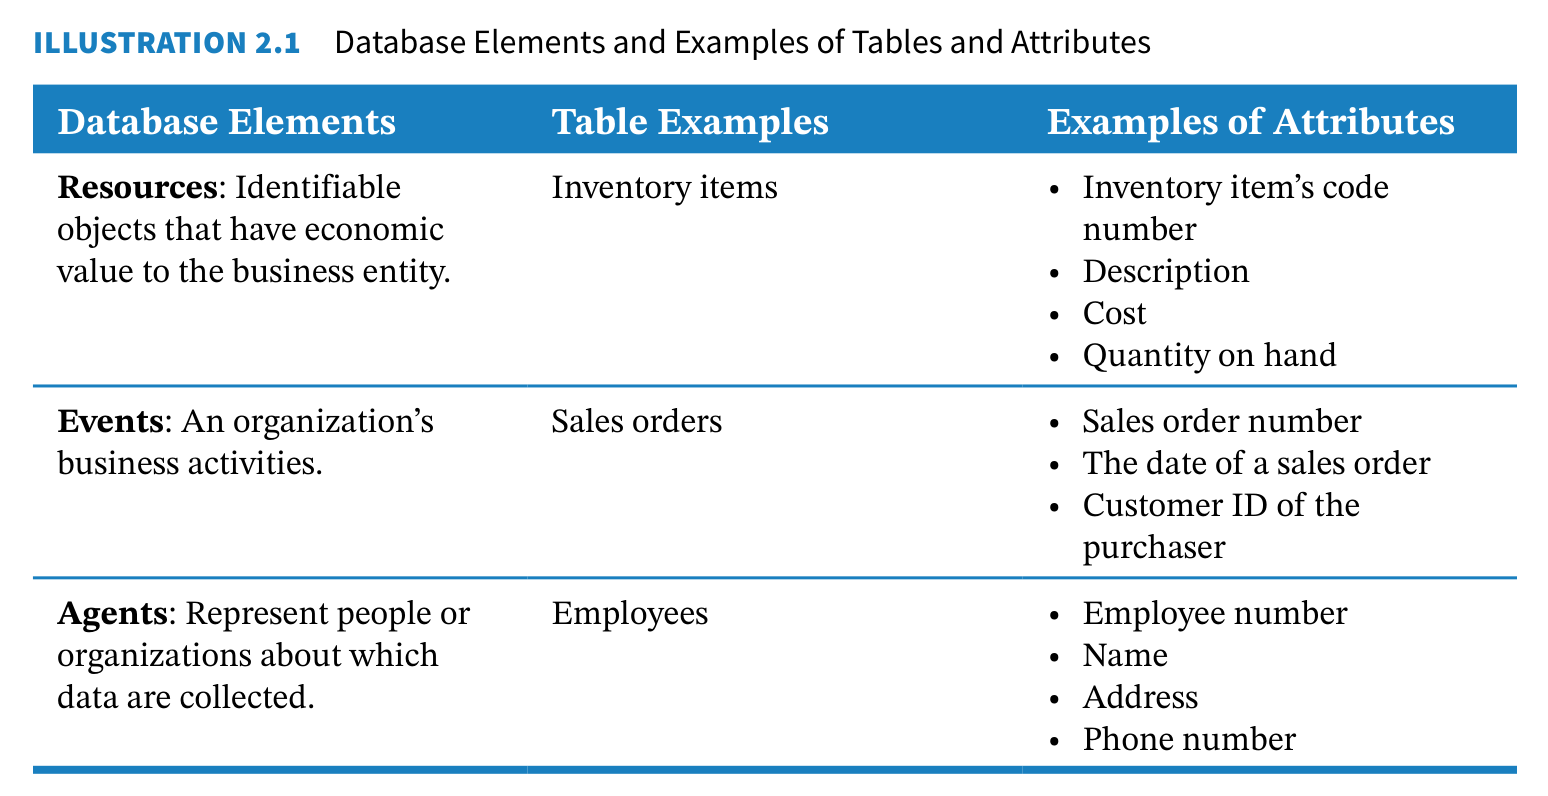
\includegraphics[height=0.65\textheight]{../textbookForPractice/Figures/Ch_02/ILLUSTRATION 2.1.png}
        \caption{Lưu trữ dữ liệu trong cơ sở dữ liệu quan hệ.}
    \end{figure}
\end{frame}

\begin{frame}{Bảng Dữ liệu \& Thuộc tính (Tables \& Attributes)}
    \begin{figure}[h]
        \centering
        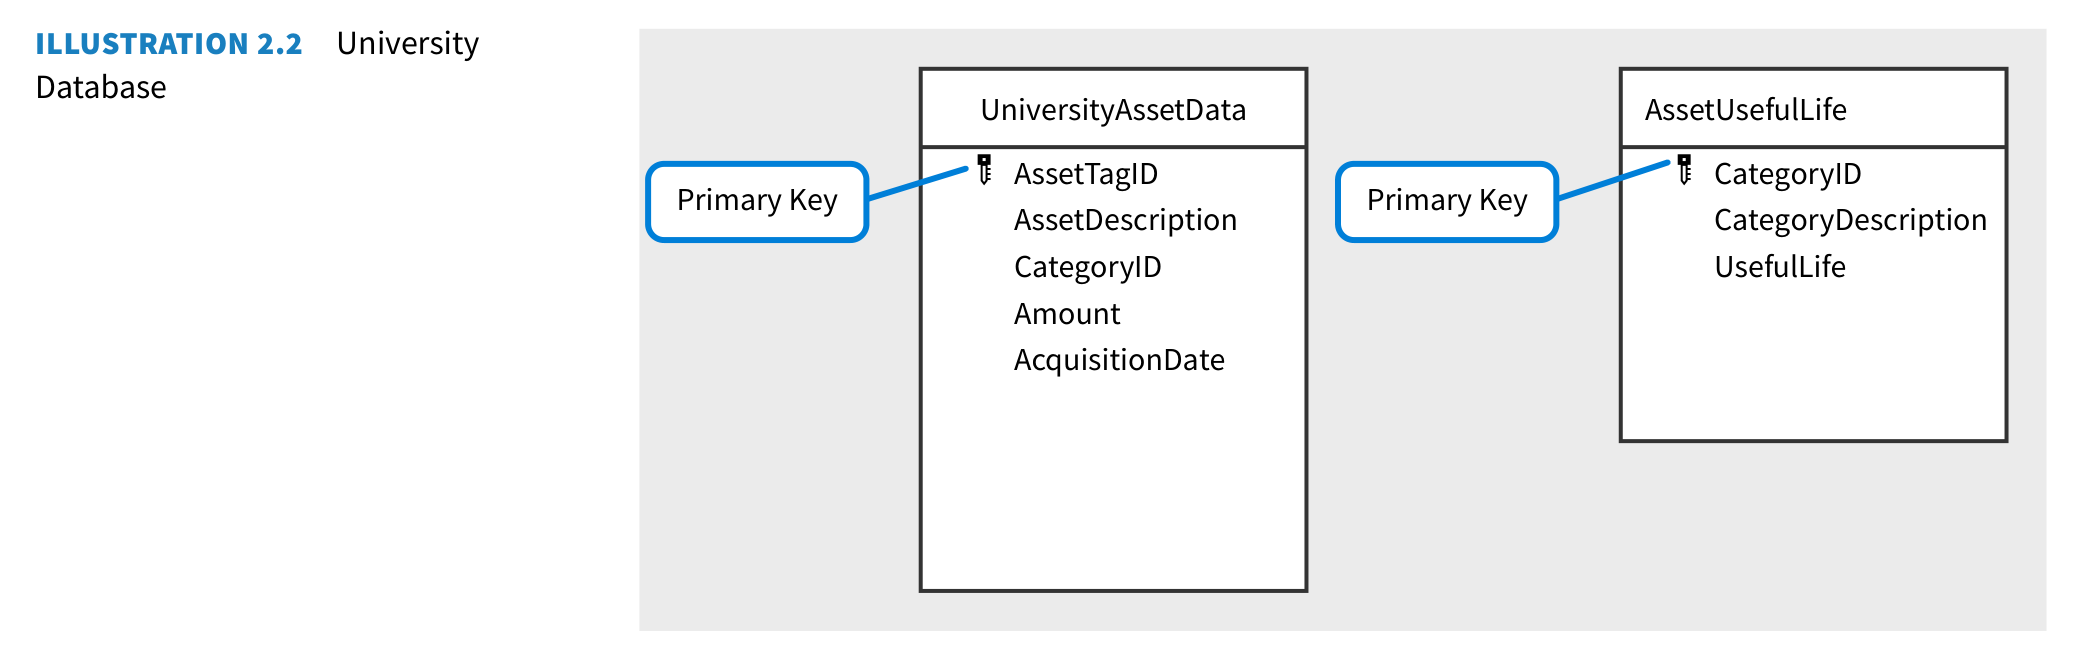
\includegraphics[height=0.55\textheight]{../textbookForPractice/Figures/Ch_02/ILLUSTRATION 2.2.png}
        \caption{Bảng dữ liệu Tài sản với các Thuộc tính (Cột) và Bản ghi (Hàng).}
    \end{figure}
    \begin{itemize}
        \item Mỗi \textbf{Cột (Column)} đại diện cho một thuộc tính.
        \item Mỗi \textbf{Hàng (Row)} là một bản ghi duy nhất.
    \end{itemize}
\end{frame}

\begin{frame}{Khóa chính (Primary Key) \& Khóa ngoại (Foreign Key)}
    \begin{figure}[h]
        \centering
        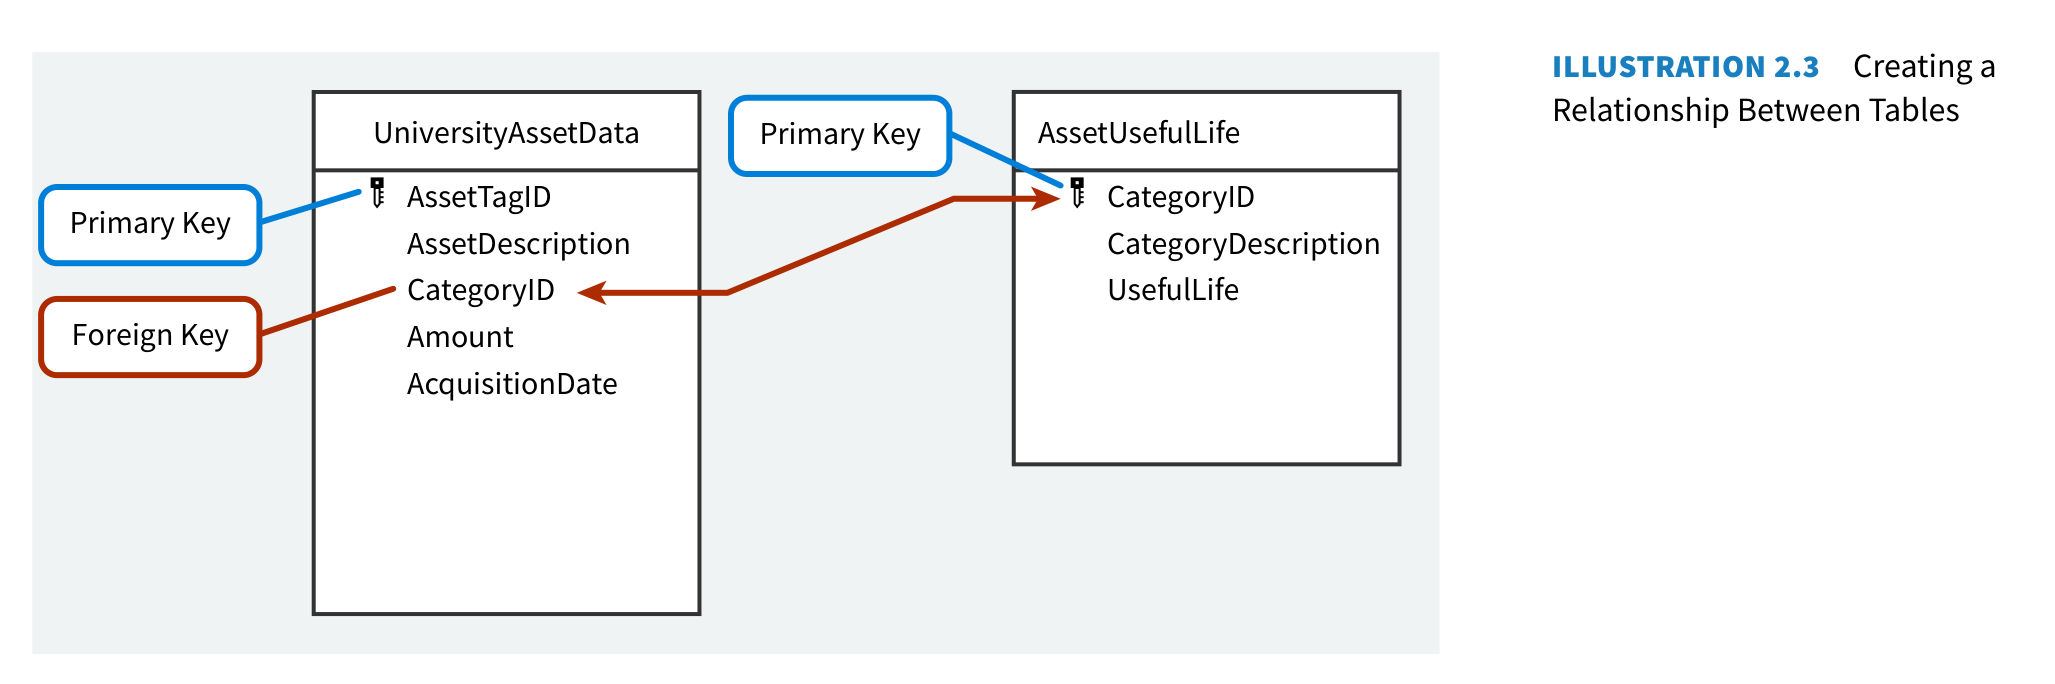
\includegraphics[height=0.55\textheight]{../textbookForPractice/Figures/Ch_02/ILLUSTRATION 2.3.png}
        \caption{Mối quan hệ giữa Bảng Tài sản và Bảng Danh mục.}
    \end{figure}
    \begin{itemize}
        \item \textbf{Khóa chính (PK):} Định danh duy nhất cho mỗi bản ghi trong bảng (vd: Asset ID).
        \item \textbf{Khóa ngoại (FK):} Tham chiếu đến Khóa chính của bảng khác để tạo mối liên kết (vd: Category ID).
    \end{itemize}
\end{frame}

\begin{frame}{Kết nối các bảng (Joining Tables)}
    \begin{figure}[h]
        \centering
        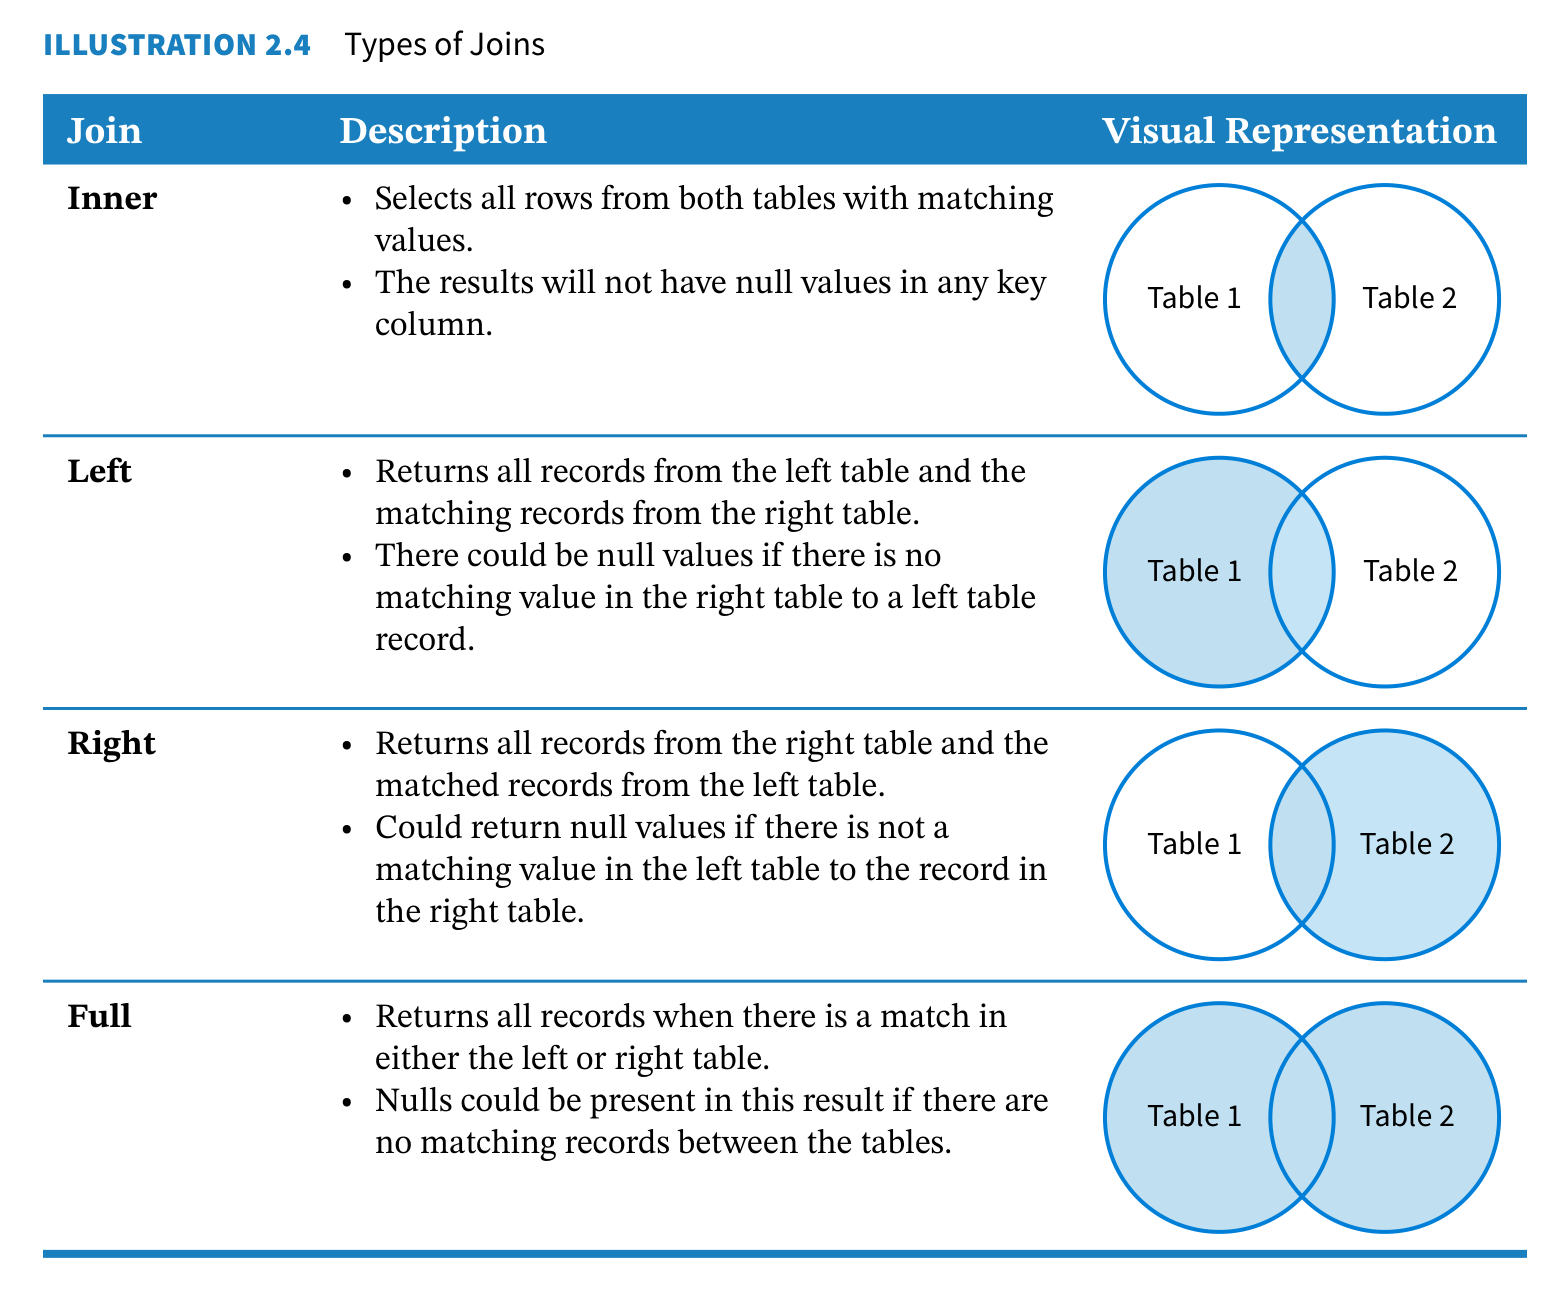
\includegraphics[height=0.6\textheight]{../textbookForPractice/Figures/Ch_02/Table 1 Table 2 column.png}
        \caption{Các loại kết nối: Inner, Left, Right, Full Outer Join.}
    \end{figure}
\end{frame}

\begin{frame}{Ví dụ Inner Join \& Left Join (Bikes R Us)}
    \begin{columns}
        \begin{column}{0.5\textwidth}
            \begin{figure}[h]
                \centering
                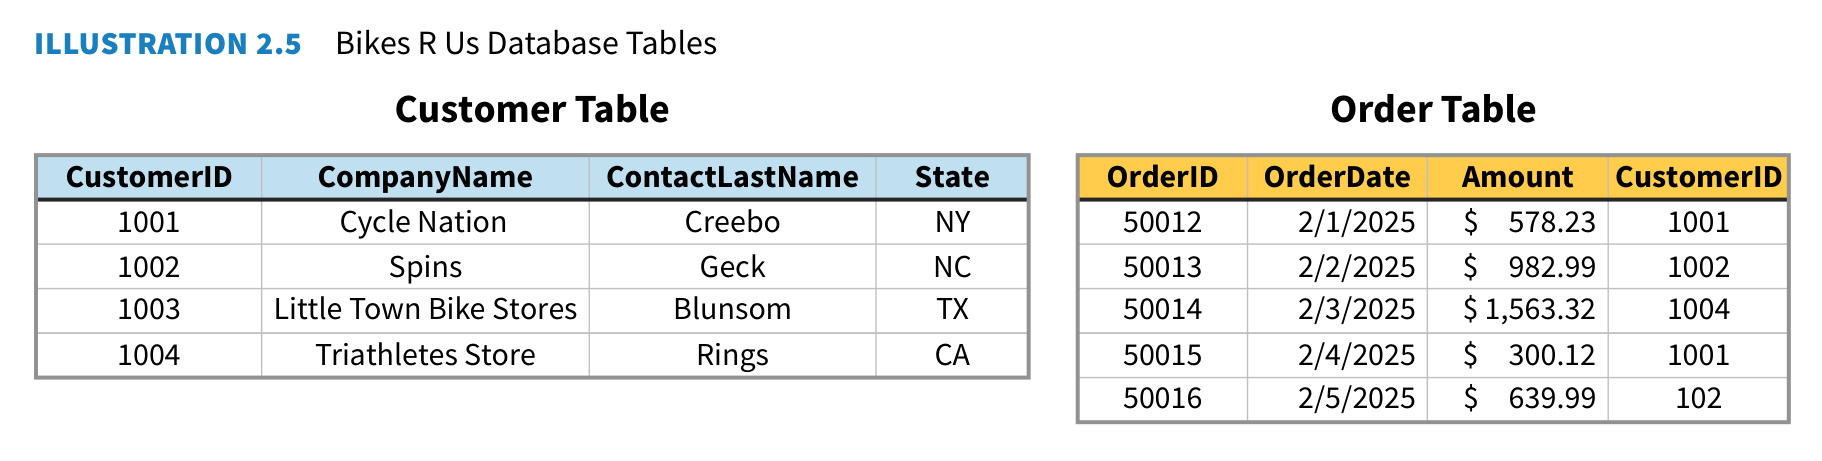
\includegraphics[width=\textwidth]{../textbookForPractice/Figures/Ch_02/ILLUSTRATION 2.5.png}
                \caption{Bảng ban đầu: Table 1 \& 2.}
            \end{figure}
        \end{column}
        \begin{column}{0.5\textwidth}
            \begin{figure}[h]
                \centering
                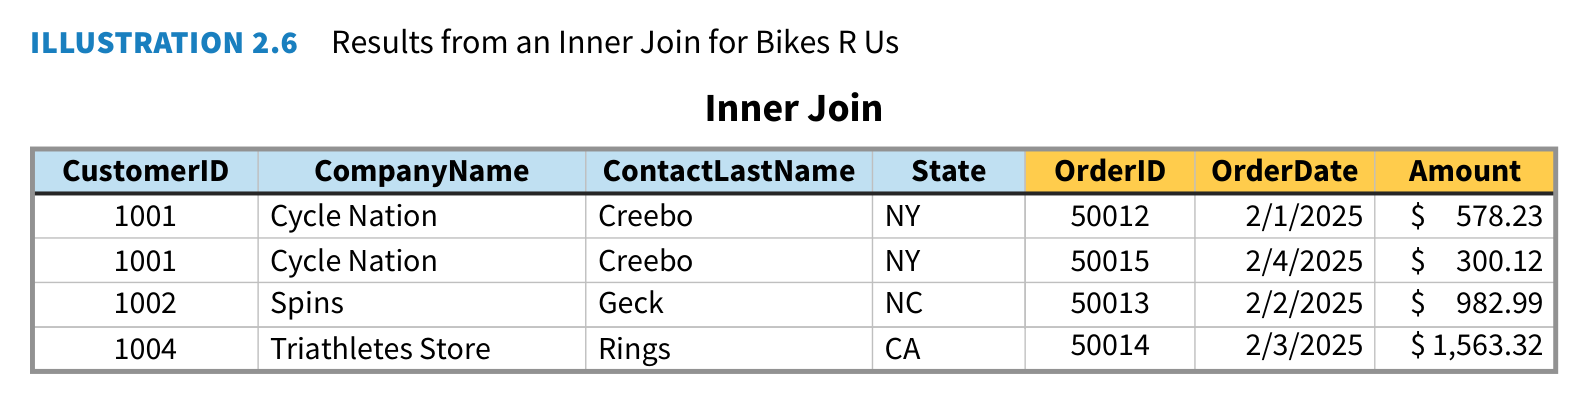
\includegraphics[width=\textwidth]{../textbookForPractice/Figures/Ch_02/ILLUSTRATION 2.6.png}
                \caption{Inner Join (Chỉ các bản ghi khớp).}
            \end{figure}
            \begin{figure}[h]
                \centering
                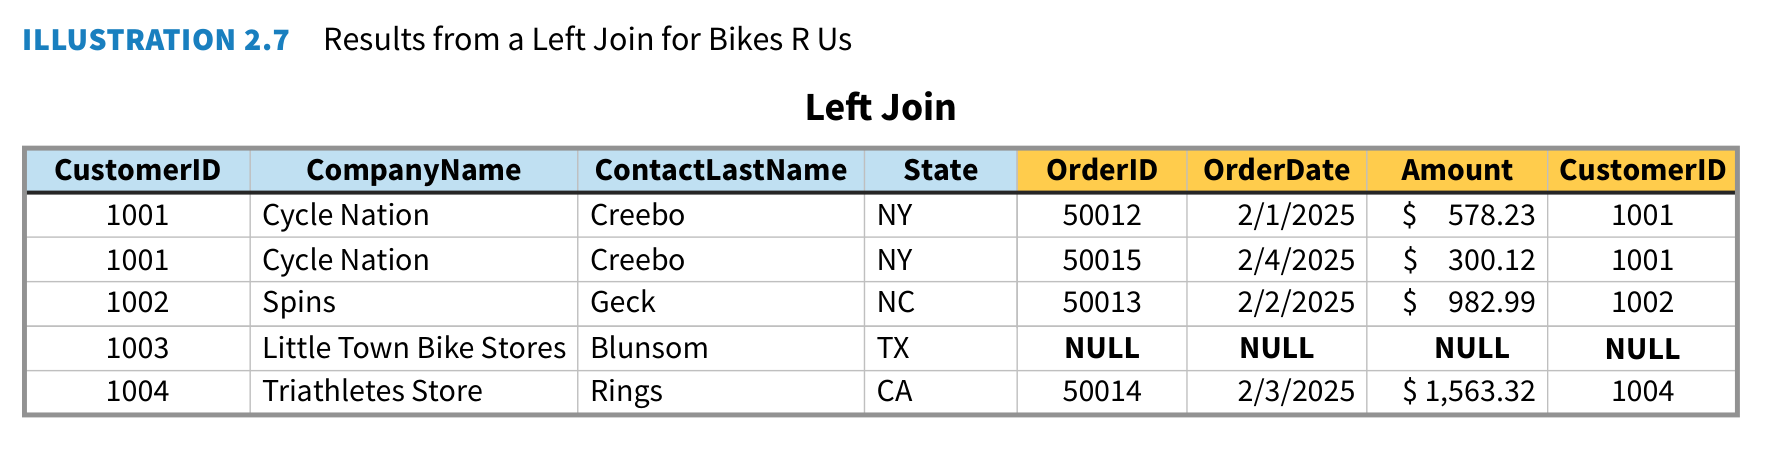
\includegraphics[width=\textwidth]{../textbookForPractice/Figures/Ch_02/ILLUSTRATION 2.7.png}
                \caption{Left Join (Tất cả từ Table 1).}
            \end{figure}
        \end{column}
    \end{columns}
\end{frame}

\begin{frame}{Áp dụng (Apply It 2.1) - Hệ thống Thông tin Kế toán Super Scooters}
    \begin{figure}[h]
        \centering
        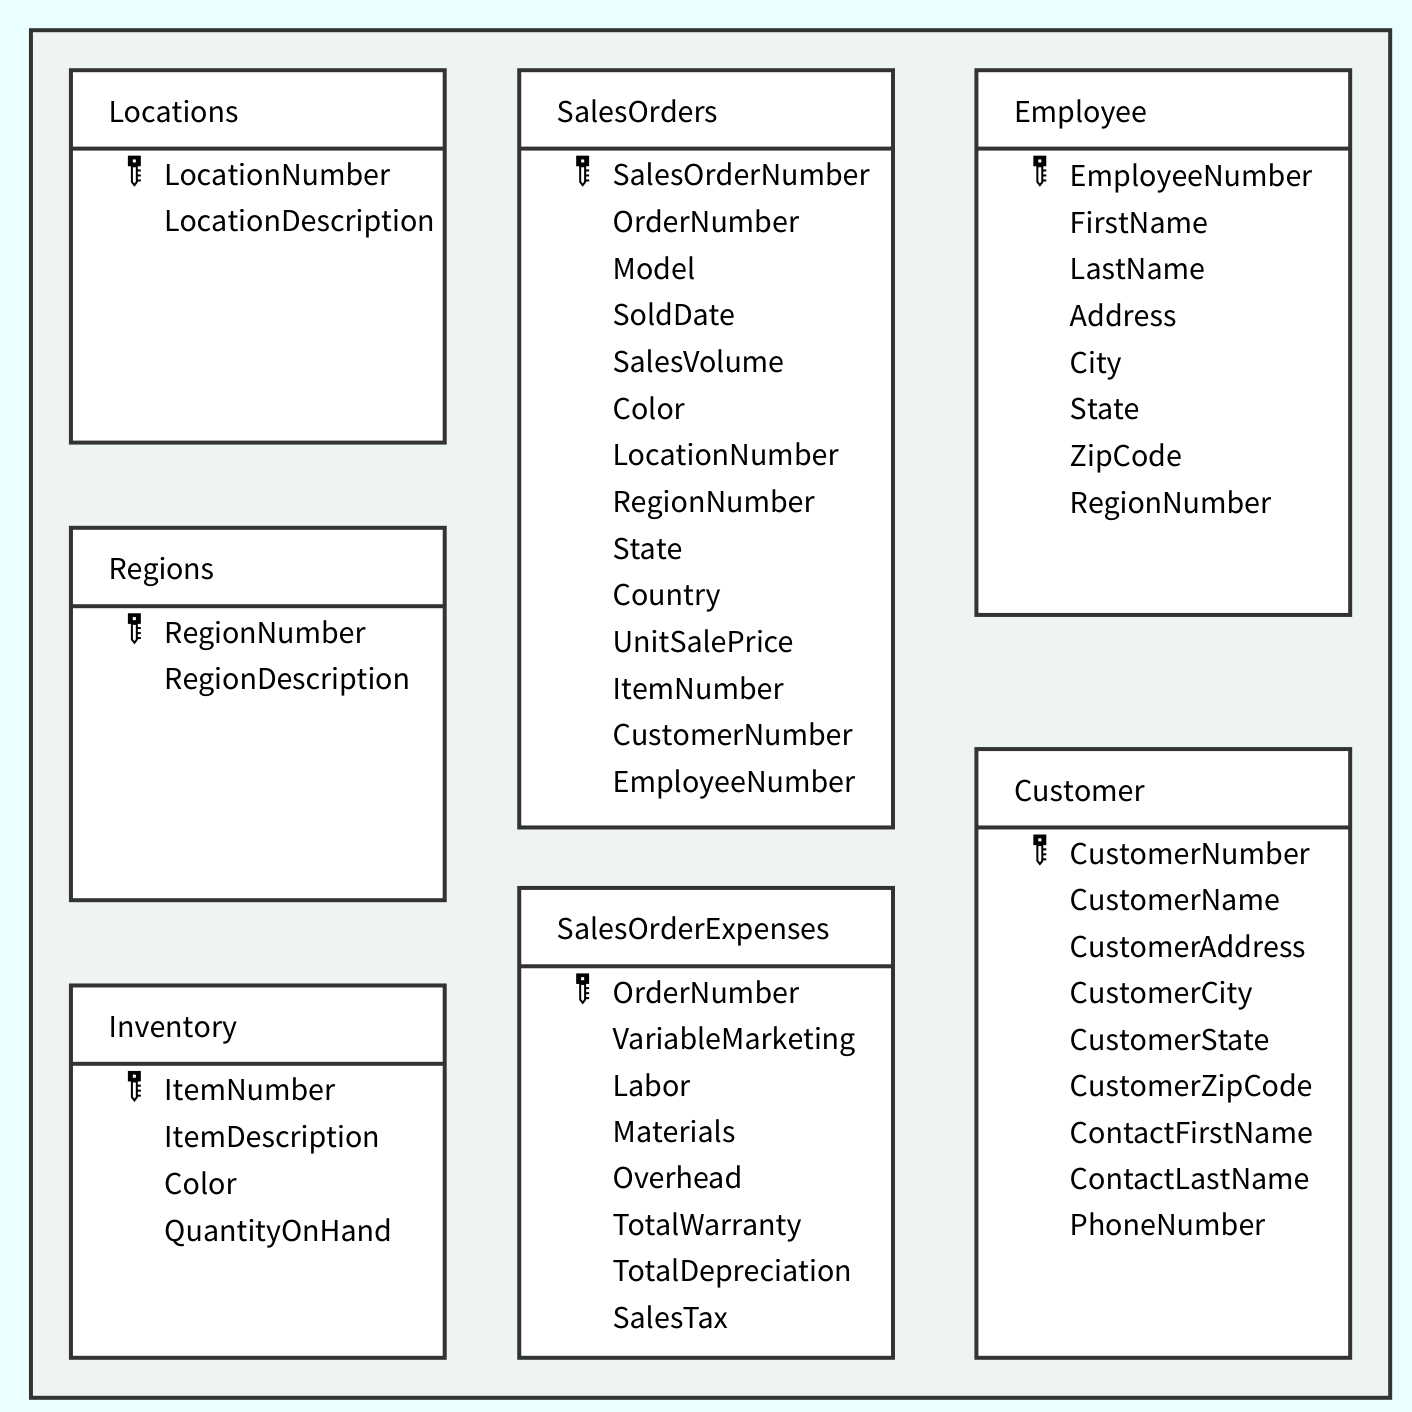
\includegraphics[height=0.65\textheight]{../textbookForPractice/Figures/Ch_02/Apply It 2.1.png}
        \caption{Nhận diện PK và FK trong sơ đồ dữ liệu (Data Dictionary).}
    \end{figure}
\end{frame}

% --- Phần 2: Các Hàm Bảng Tính (LO 2.2) ---
\begin{frame}{2.2 Các Hàm Bảng Tính Phân Tích Lượng Lớn Dữ Liệu}
    \begin{itemize}
        \item Bảng tính (Spreadsheets) như Microsoft Excel là công cụ phân tích phổ biến nhất đối với kế toán viên.
        \item Các hàm giúp chúngạn \textbf{thao tác, làm sạch, và phân tích} hàng ngàn dòng dữ liệu một cách tự động.
        \item \textbf{Cú pháp chung:} \texttt{=TênHàm(Đối số 1, Đối số 2, ...)}
    \end{itemize}
\end{frame}

\begin{frame}{Các Hàm Cơ bản Phổ biến (1/2)}
    \begin{figure}[h]
        \centering
        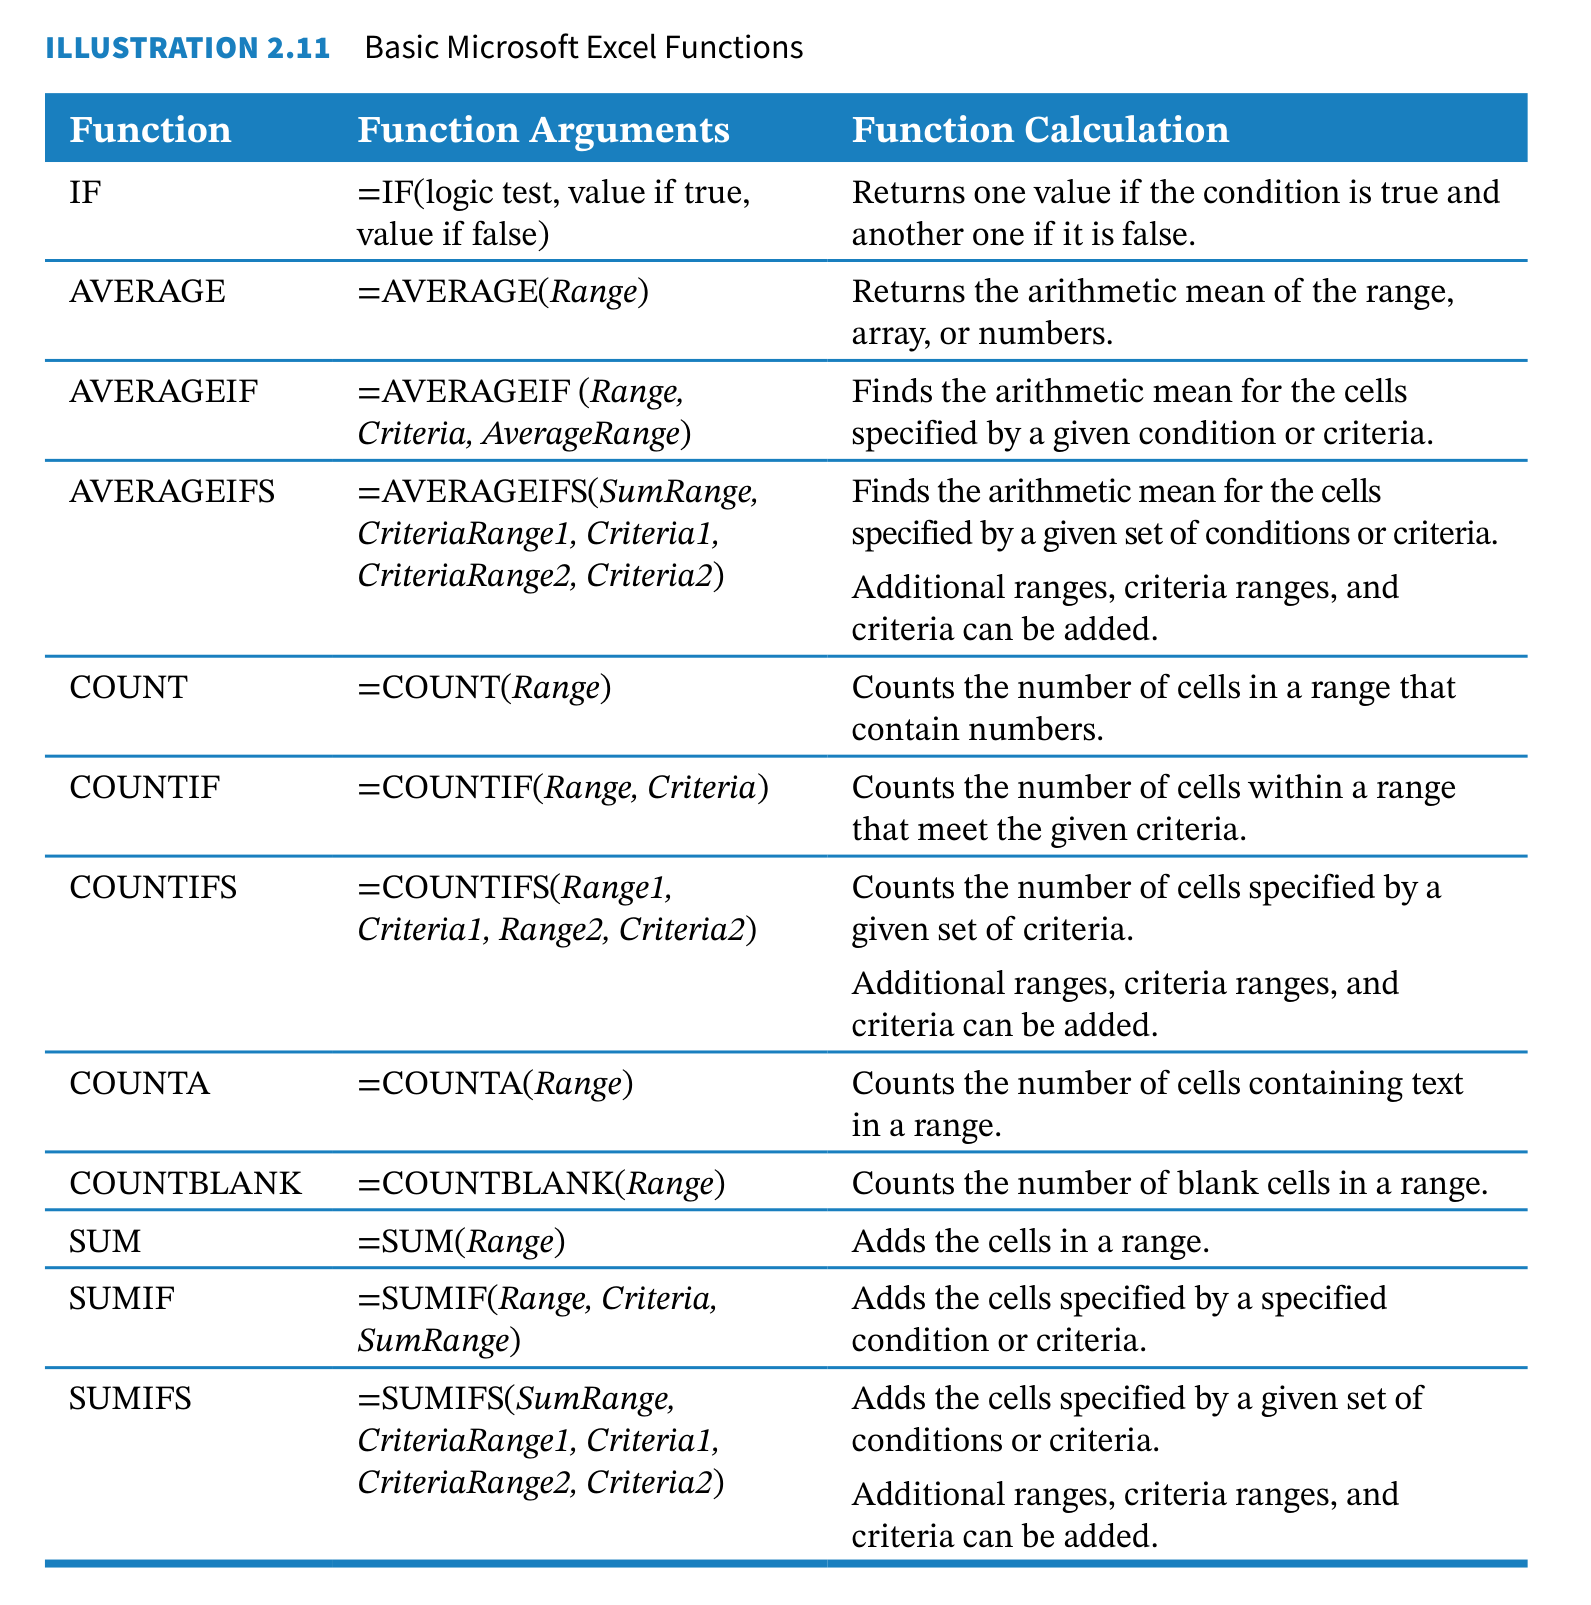
\includegraphics[height=0.65\textheight]{../textbookForPractice/Figures/Ch_02/ILLUSTRATION 2.11.png}
        \caption{Các hàm Toán học, Thống kê \& Logic cơ bản.}
    \end{figure}
\end{frame}

\begin{frame}{Sử dụng Hộp Đối số Hàm (Function Arguments)}
    \begin{columns}
        \begin{column}{0.5\textwidth}
            \begin{figure}[h]
                \centering
                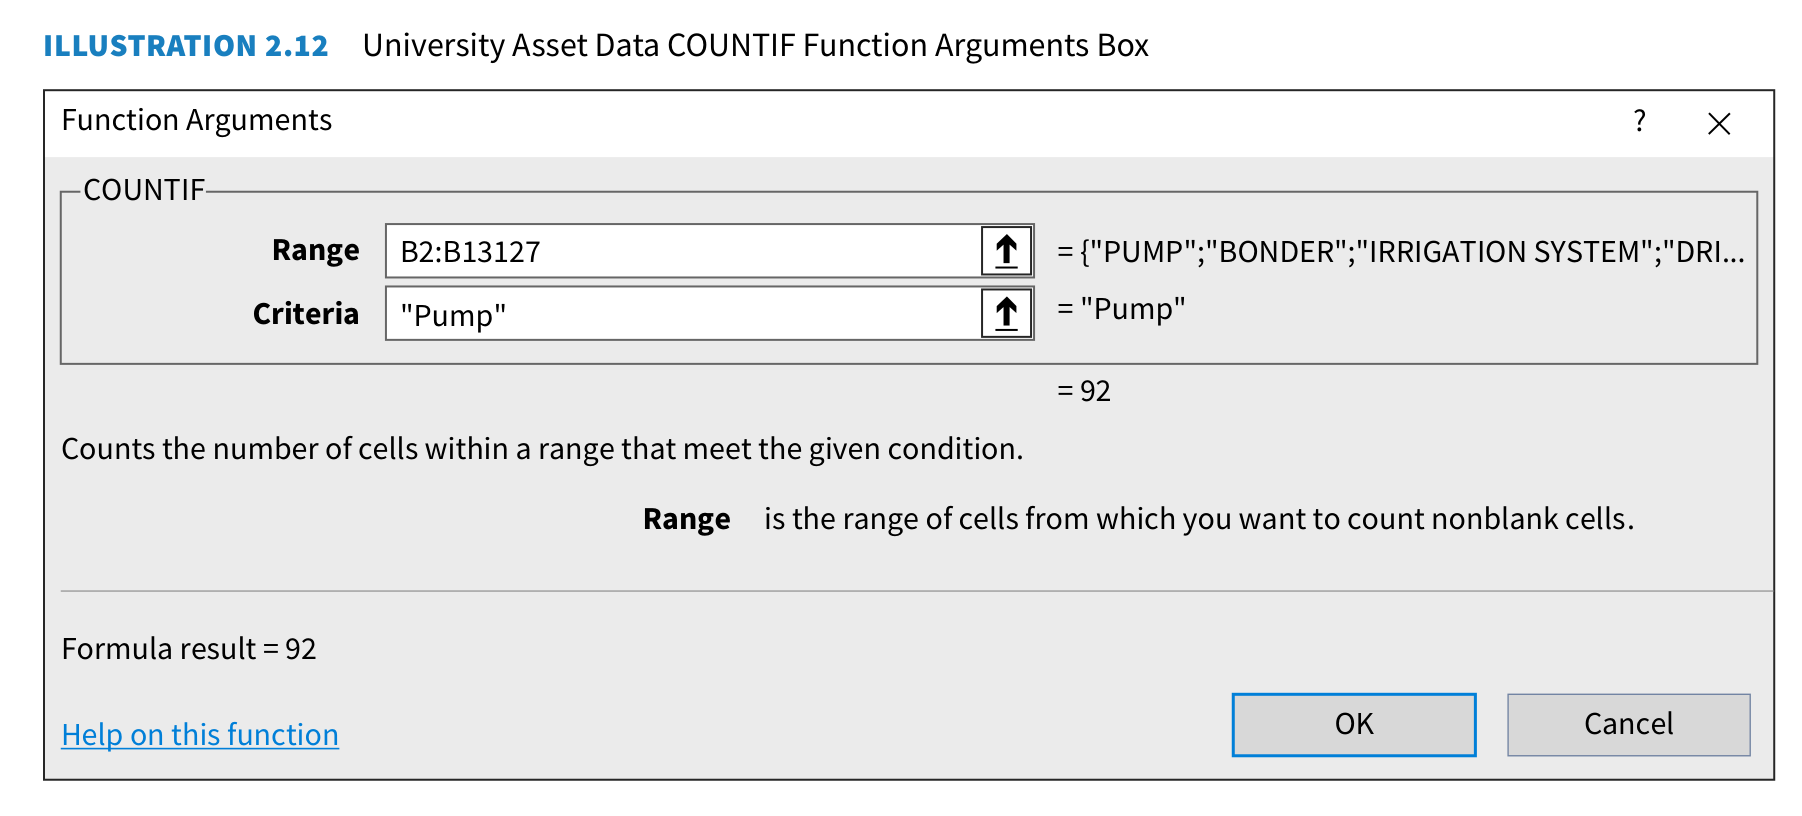
\includegraphics[width=\textwidth]{../textbookForPractice/Figures/Ch_02/ILLUSTRATION 2.12.png}
                \caption{Chèn hàm (Insert Function).}
            \end{figure}
        \end{column}
        \begin{column}{0.5\textwidth}
            \begin{figure}[h]
                \centering
                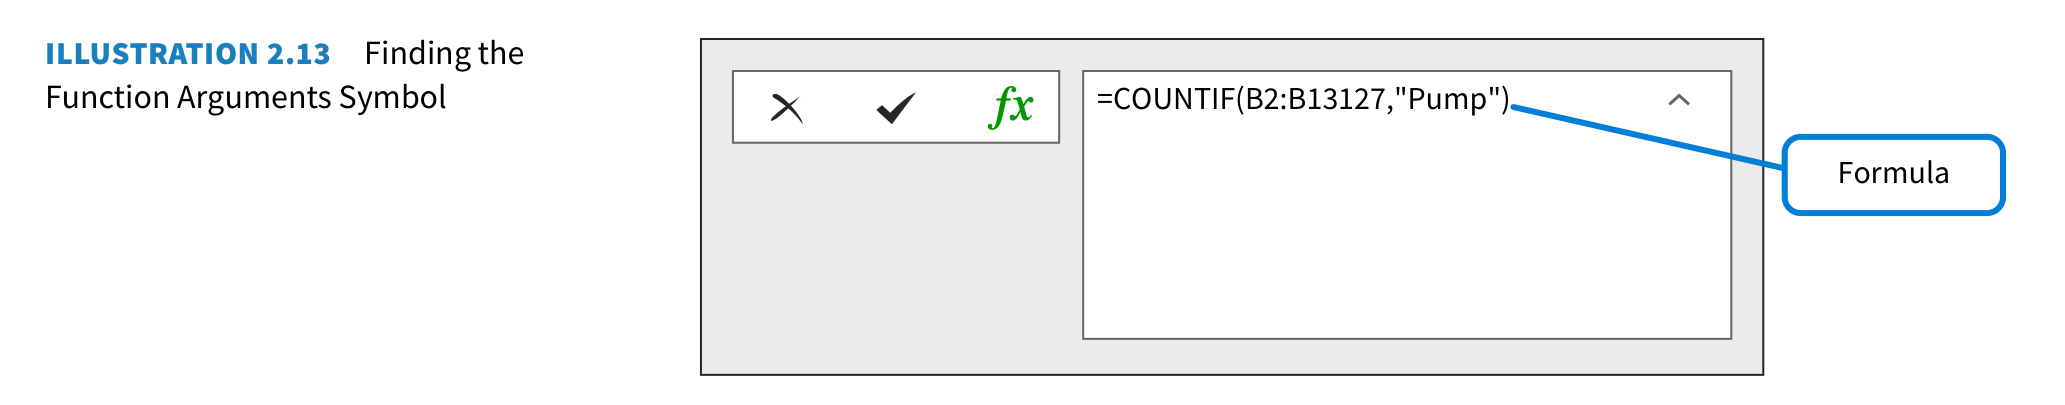
\includegraphics[width=\textwidth]{../textbookForPractice/Figures/Ch_02/ILLUSTRATION 2.13.png}
                \caption{Hộp thoại khai báo các đối số trực quan.}
            \end{figure}
        \end{column}
    \end{columns}
\end{frame}

\begin{frame}{Áp dụng Các Hàm Cơ bản của Excel}
    \begin{figure}[h]
        \centering
        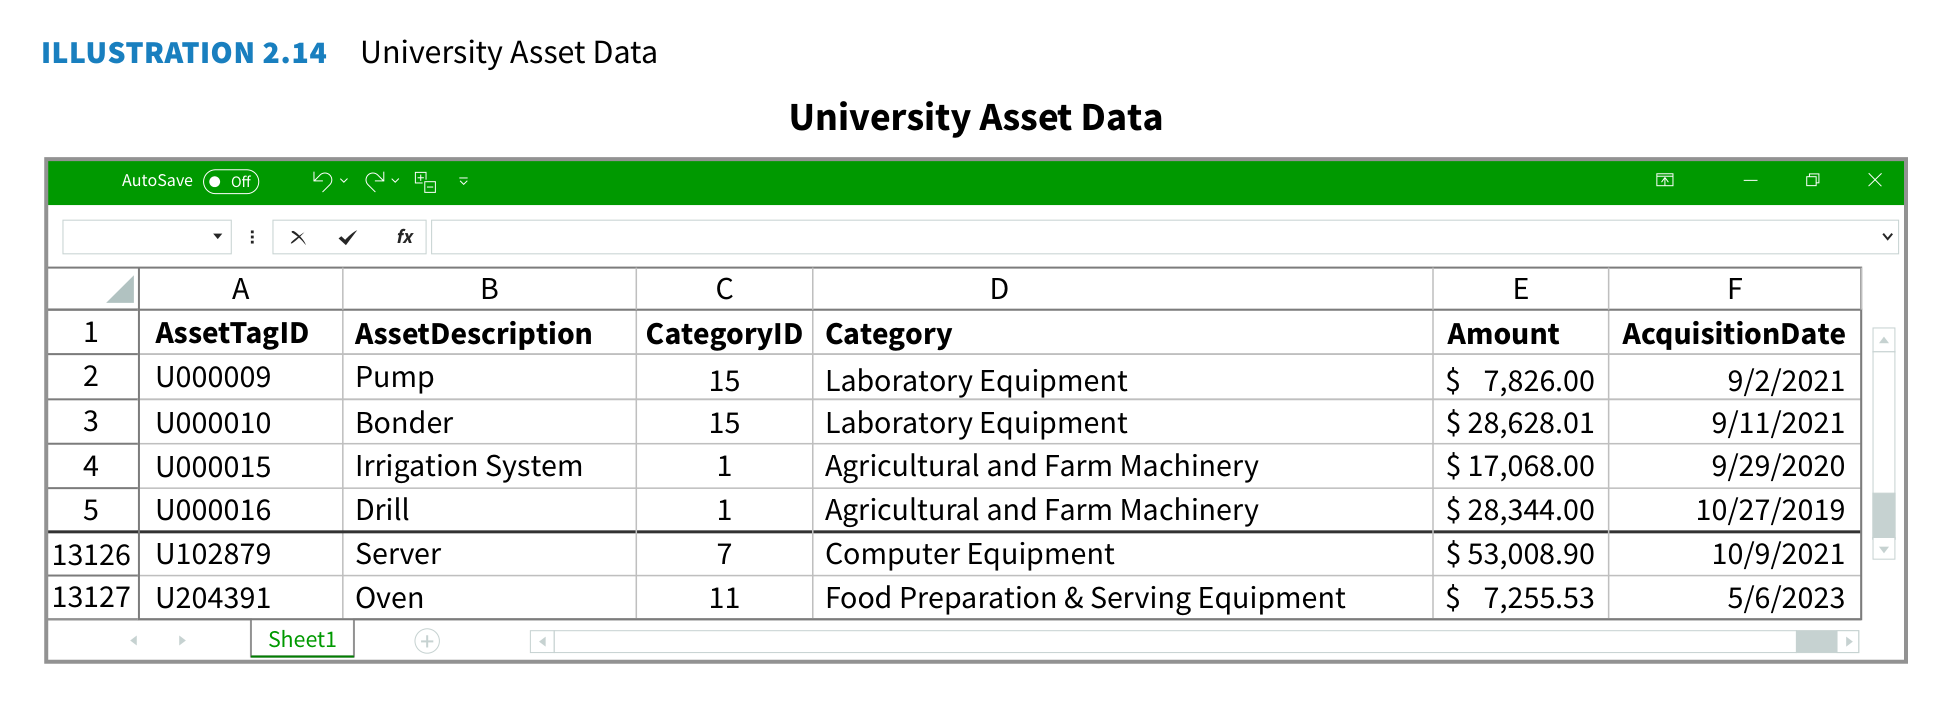
\includegraphics[height=0.65\textheight]{../textbookForPractice/Figures/Ch_02/ILLUSTRATION 2.14.png}
        \caption{Tính Khấu hao Tích lũy (Accumulated Depreciation) bằng hàm SUM, MAX, MIN.}
    \end{figure}
\end{frame}

\begin{frame}{Trả lời Câu hỏi với Hàm (COUNTIF \& COUNTIFS)}
    \begin{columns}
        \begin{column}{0.5\textwidth}
            \begin{figure}[h]
                \centering
                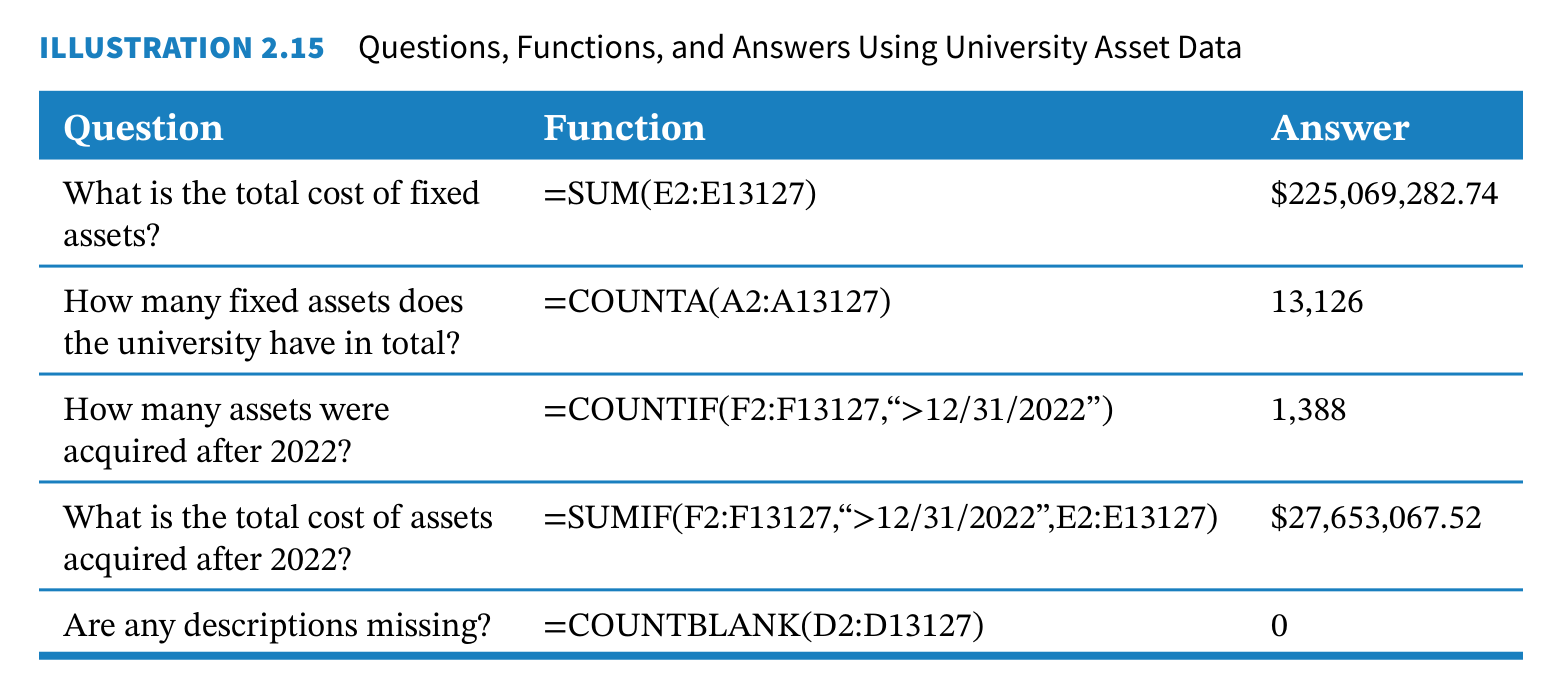
\includegraphics[width=\textwidth]{../textbookForPractice/Figures/Ch_02/ILLUSTRATION 2.15.png}
                \caption{Hàm \texttt{COUNTIFS} đếm số tài sản theo nhiều điều kiện.}
            \end{figure}
        \end{column}
        \begin{column}{0.5\textwidth}
            \begin{figure}[h]
                \centering
                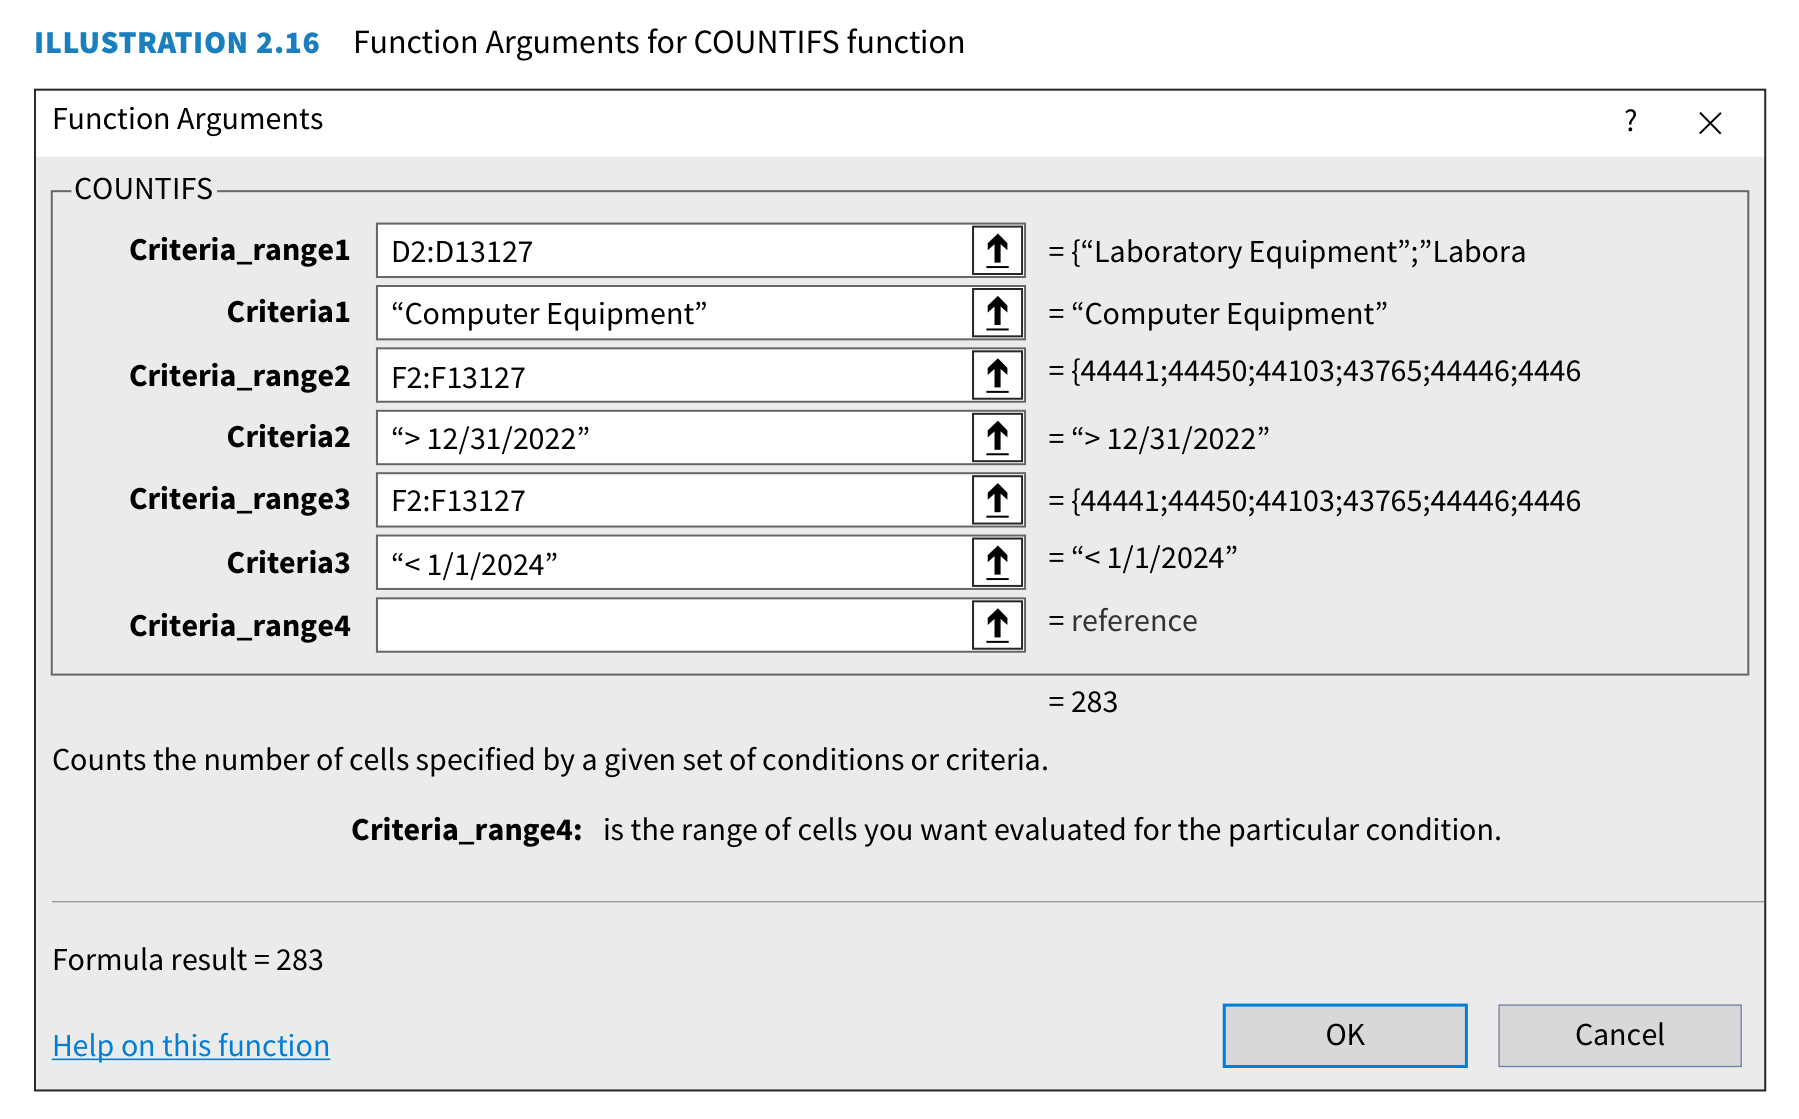
\includegraphics[width=\textwidth]{../textbookForPractice/Figures/Ch_02/ILLUSTRATION 2.16.png}
                \caption{Kết quả: Có 5 Máy chủ Laptop Dell chưa được phân bổ.}
            \end{figure}
        \end{column}
    \end{columns}
\end{frame}

\begin{frame}{Áp dụng (Apply It 2.2) - Phân tích Bán hàng (Super Scooters)}
    \begin{figure}[h]
        \centering
        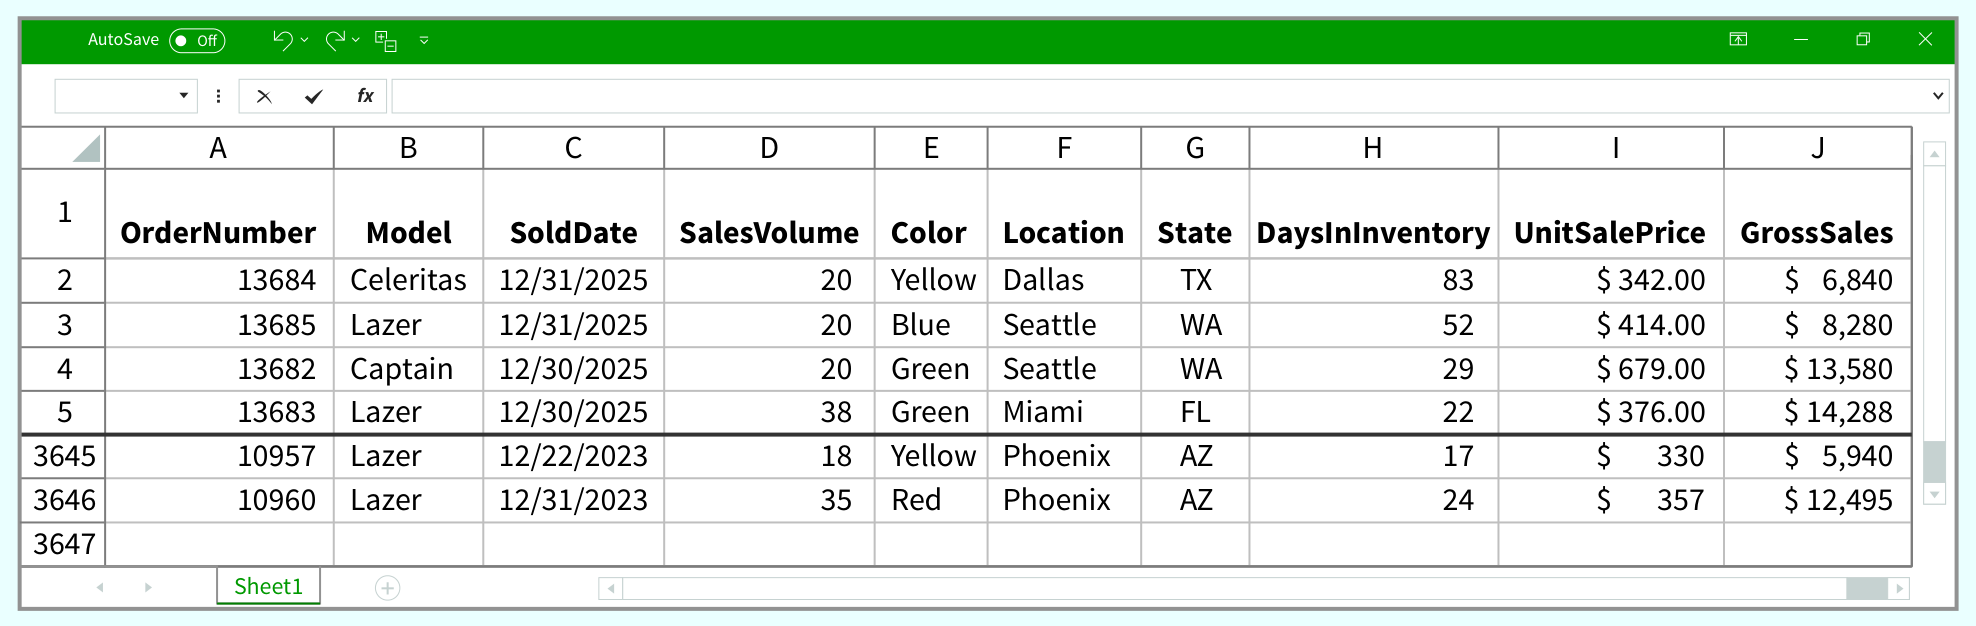
\includegraphics[height=0.65\textheight]{../textbookForPractice/Figures/Ch_02/Apply It 2.2.png}
        \caption{Sử dụng VLOOKUP, SUM, SUMIF để tổng hợp dữ liệu giao dịch.}
    \end{figure}
\end{frame}

% --- Phần 3: Pivot Tables (LO 2.3) ---
\begin{frame}{2.3 Tổ Chức Các Tập Dữ Liệu: Pivot Tables}
    \begin{itemize}
        \item \textbf{PivotTable} là một công cụ tương tác mạnh mẽ dùng để tóm tắt và phân tích lượng dữ liệu khổng lồ.
        \item 4 Vùng làm việc chính:
        \begin{itemize}
            \item \textbf{Rows (Hàng):} Nhóm dữ liệu theo danh mục theo chiều dọc.
            \item \textbf{Columns (Cột):} Nhóm dữ liệu theo danh mục theo chiều ngang.
            \item \textbf{Values (Giá trị):} Thực hiện tính toán (SUM, COUNT, AVERAGE,...) trên các trường số liệu.
            \item \textbf{Filters (Bộ lọc):} Lọc toàn bộ PivotTable theo các điều kiện.
        \end{itemize}
    \end{itemize}
\end{frame}

\begin{frame}{Tạo một Microsoft Excel PivotTable}
    \begin{columns}
        \begin{column}{0.4\textwidth}
            \begin{figure}[h]
                \centering
                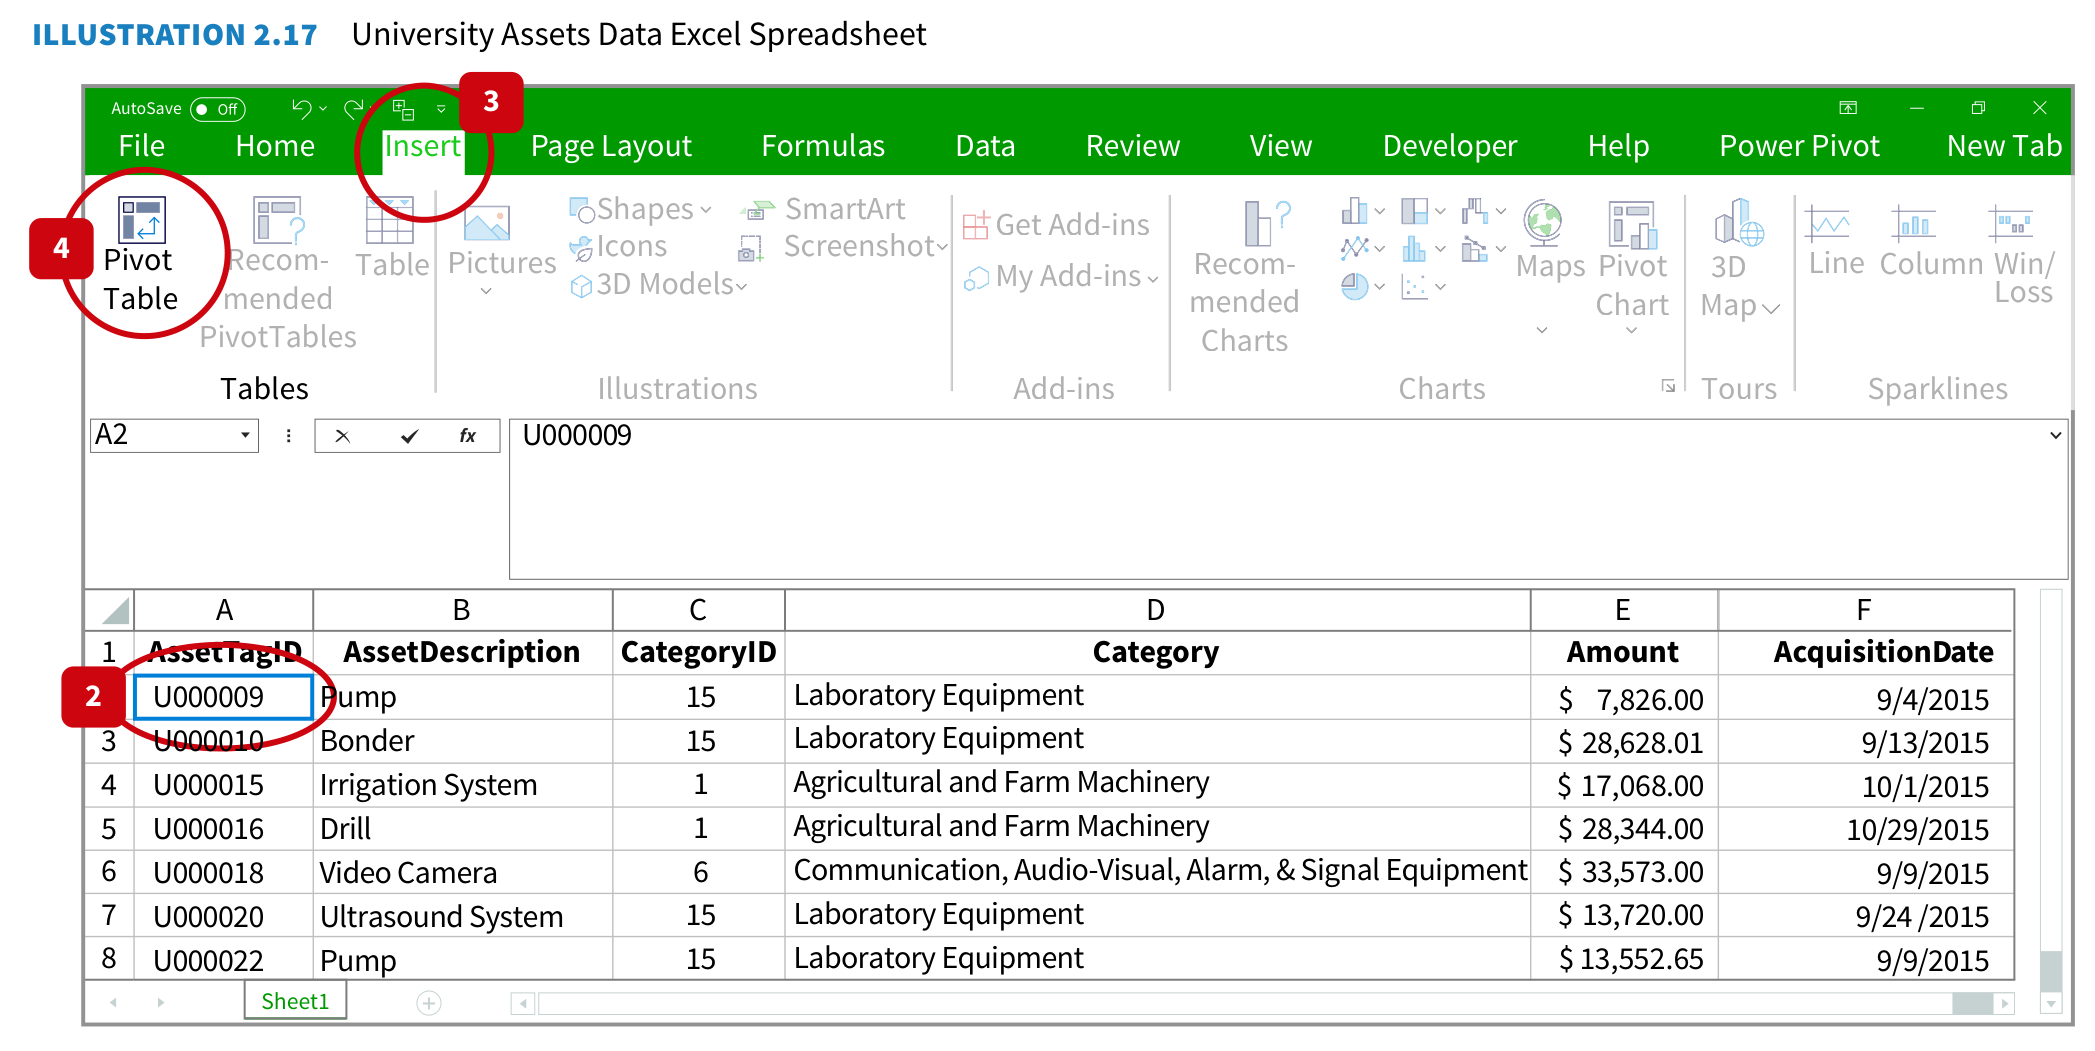
\includegraphics[width=\textwidth]{../textbookForPractice/Figures/Ch_02/ILLUSTRATION 2.17.png}
                \caption{Chọn Insert > PivotTable.}
            \end{figure}
        \end{column}
        \begin{column}{0.6\textwidth}
            \begin{figure}[h]
                \centering
                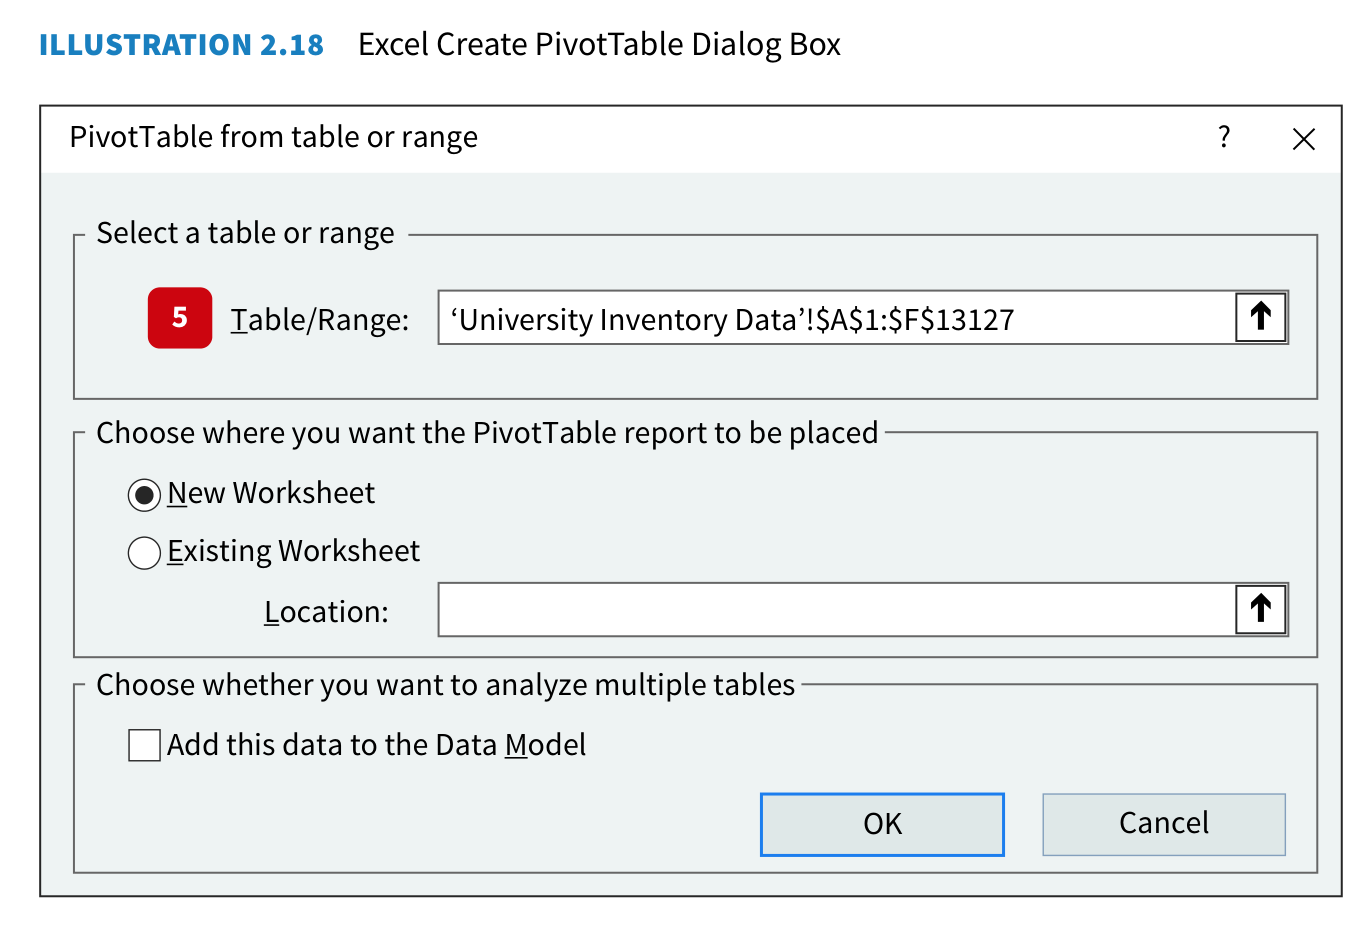
\includegraphics[width=\textwidth]{../textbookForPractice/Figures/Ch_02/ILLUSTRATION 2.18.png}
                \caption{Chọn vùng dữ liệu nguồn.}
            \end{figure}
        \end{column}
    \end{columns}
\end{frame}

\begin{frame}{Vùng làm việc PivotTable (PivotTable Fields)}
    \begin{figure}[h]
        \centering
        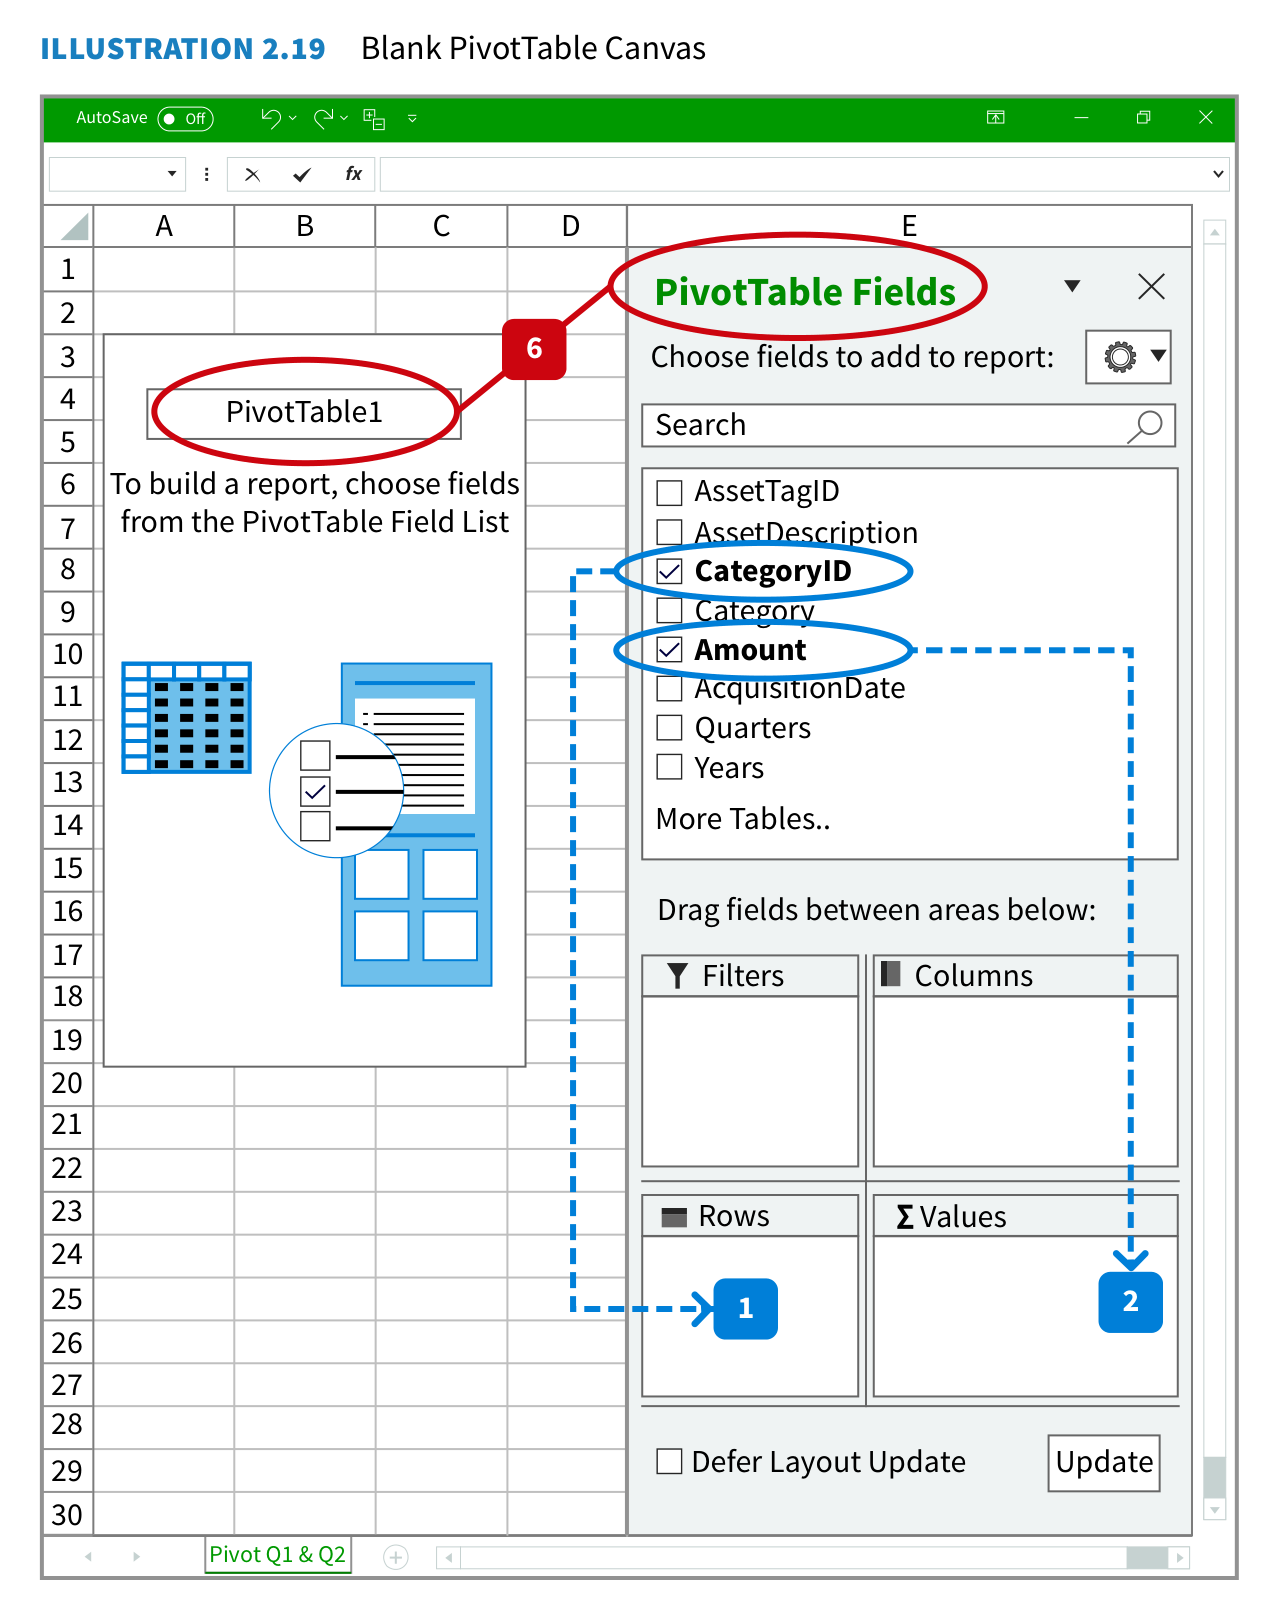
\includegraphics[height=0.65\textheight]{../textbookForPractice/Figures/Ch_02/ILLUSTRATION 2.19.png}
        \caption{Danh sách các trường (Fields) và 4 vùng (Areas) kéo thả.}
    \end{figure}
\end{frame}

\begin{frame}{Tìm Tổng Số dư theo Danh mục (Summarize Data)}
    \begin{columns}
        \begin{column}{0.5\textwidth}
            \begin{figure}[h]
                \centering
                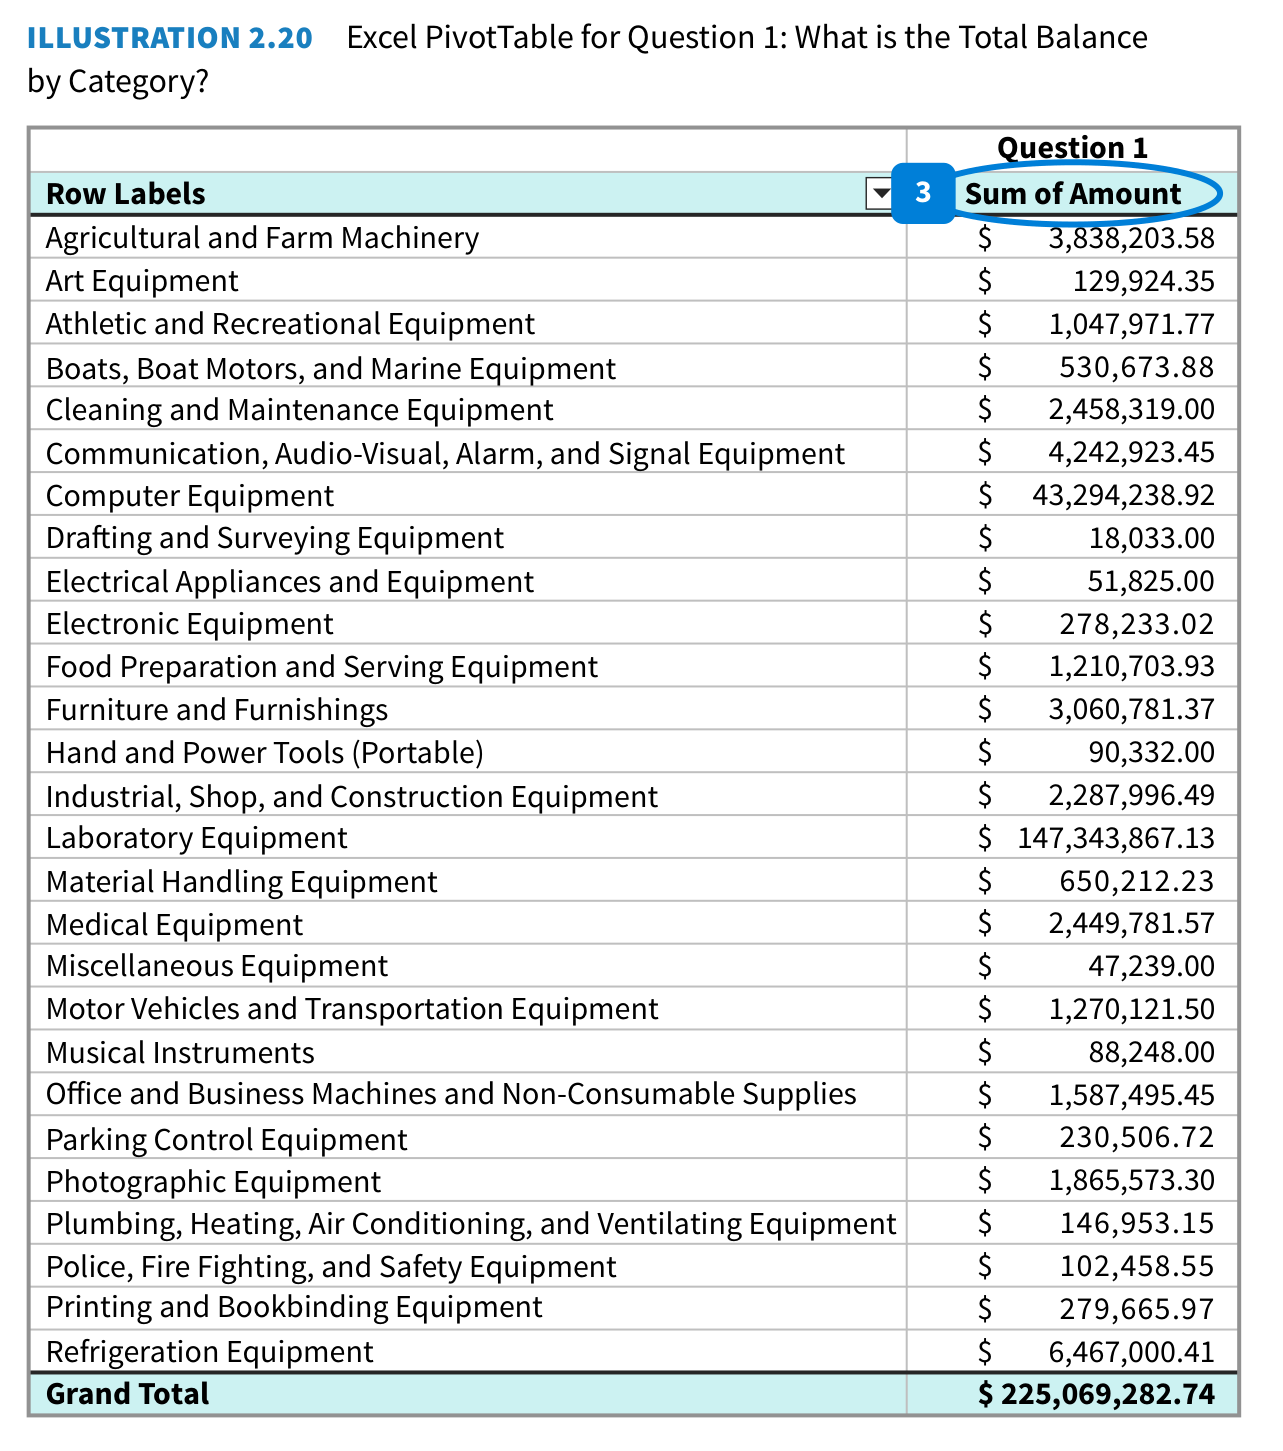
\includegraphics[width=\textwidth]{../textbookForPractice/Figures/Ch_02/ILLUSTRATION 2.20.png}
                \caption{Kéo Category vào Rows, Total Cost vào Values.}
            \end{figure}
        \end{column}
        \begin{column}{0.5\textwidth}
            \begin{figure}[h]
                \centering
                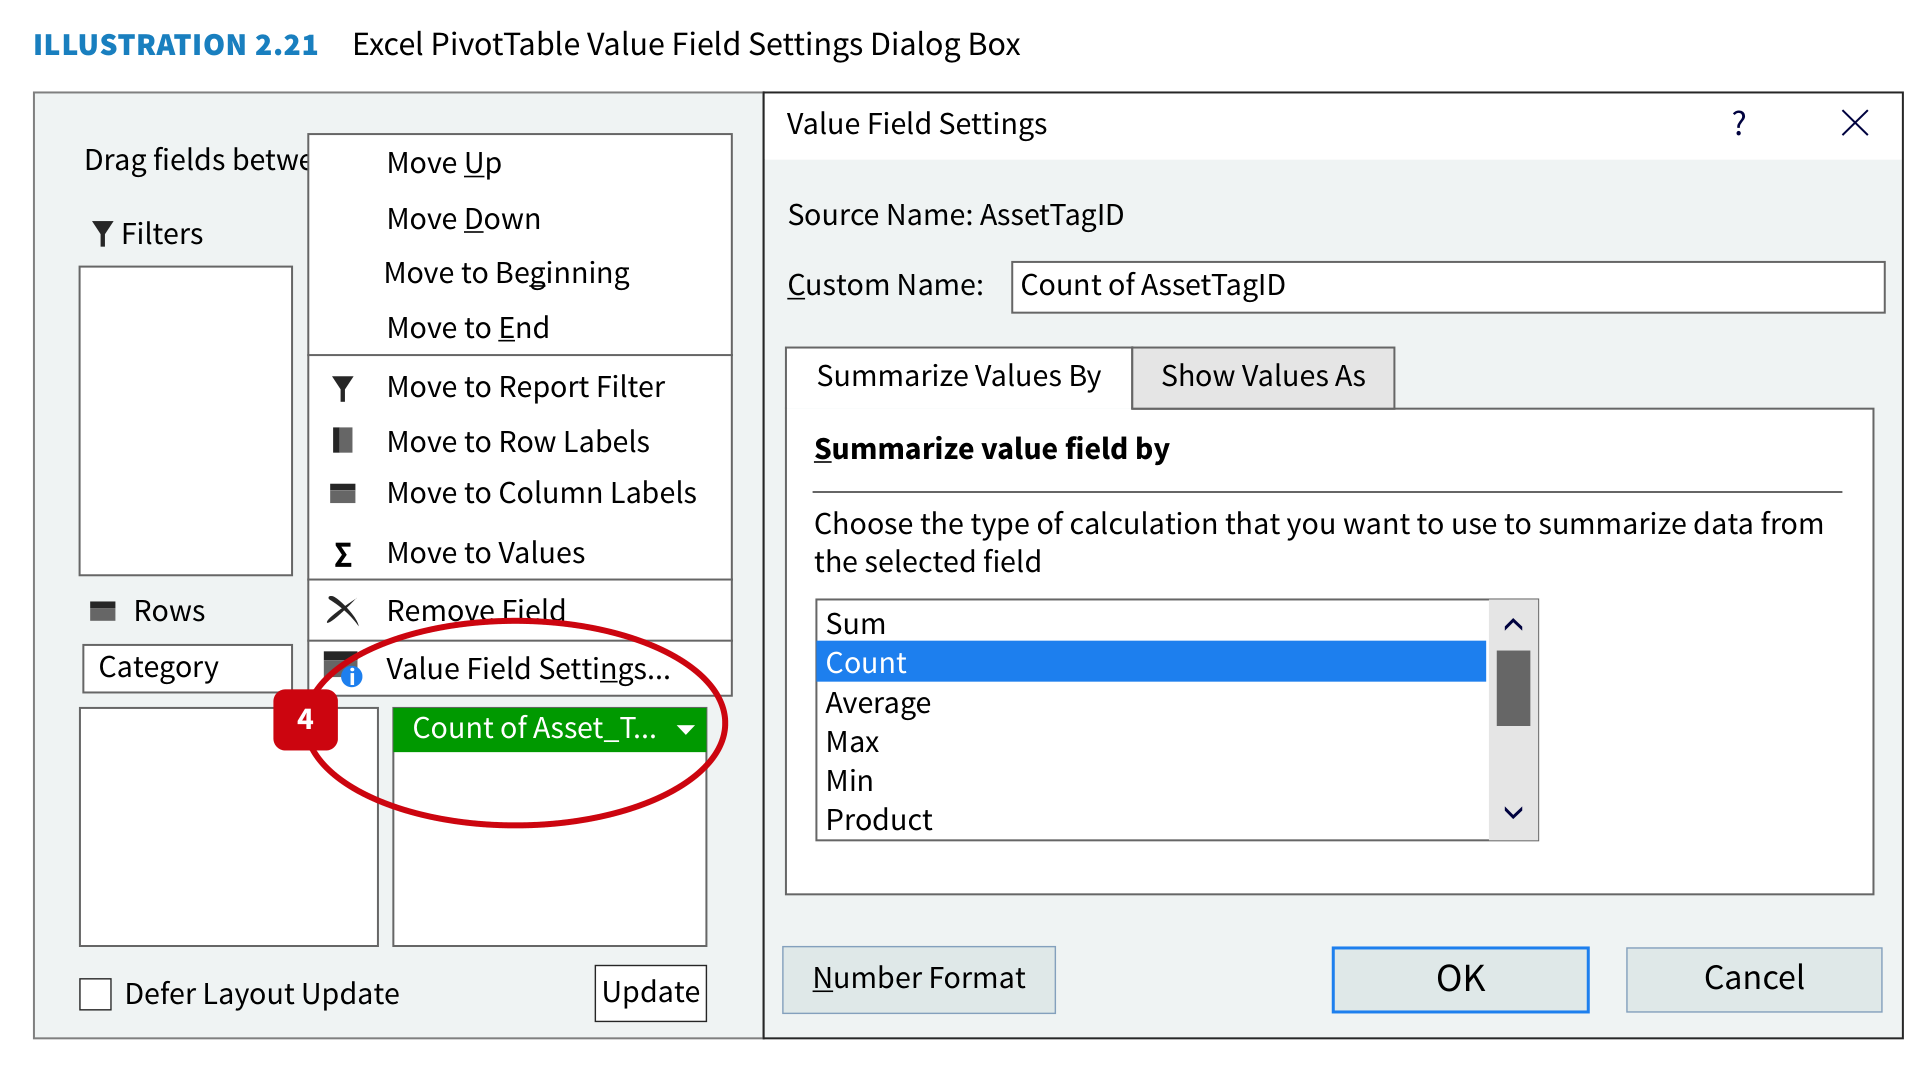
\includegraphics[width=\textwidth]{../textbookForPractice/Figures/Ch_02/ILLUSTRATION 2.21.png}
                \caption{PivotTable hiển thị Tổng chi phí theo Danh mục.}
            \end{figure}
        \end{column}
    \end{columns}
\end{frame}

\begin{frame}{Thay đổi Phép tính (Value Field Settings)}
    \begin{figure}[h]
        \centering
        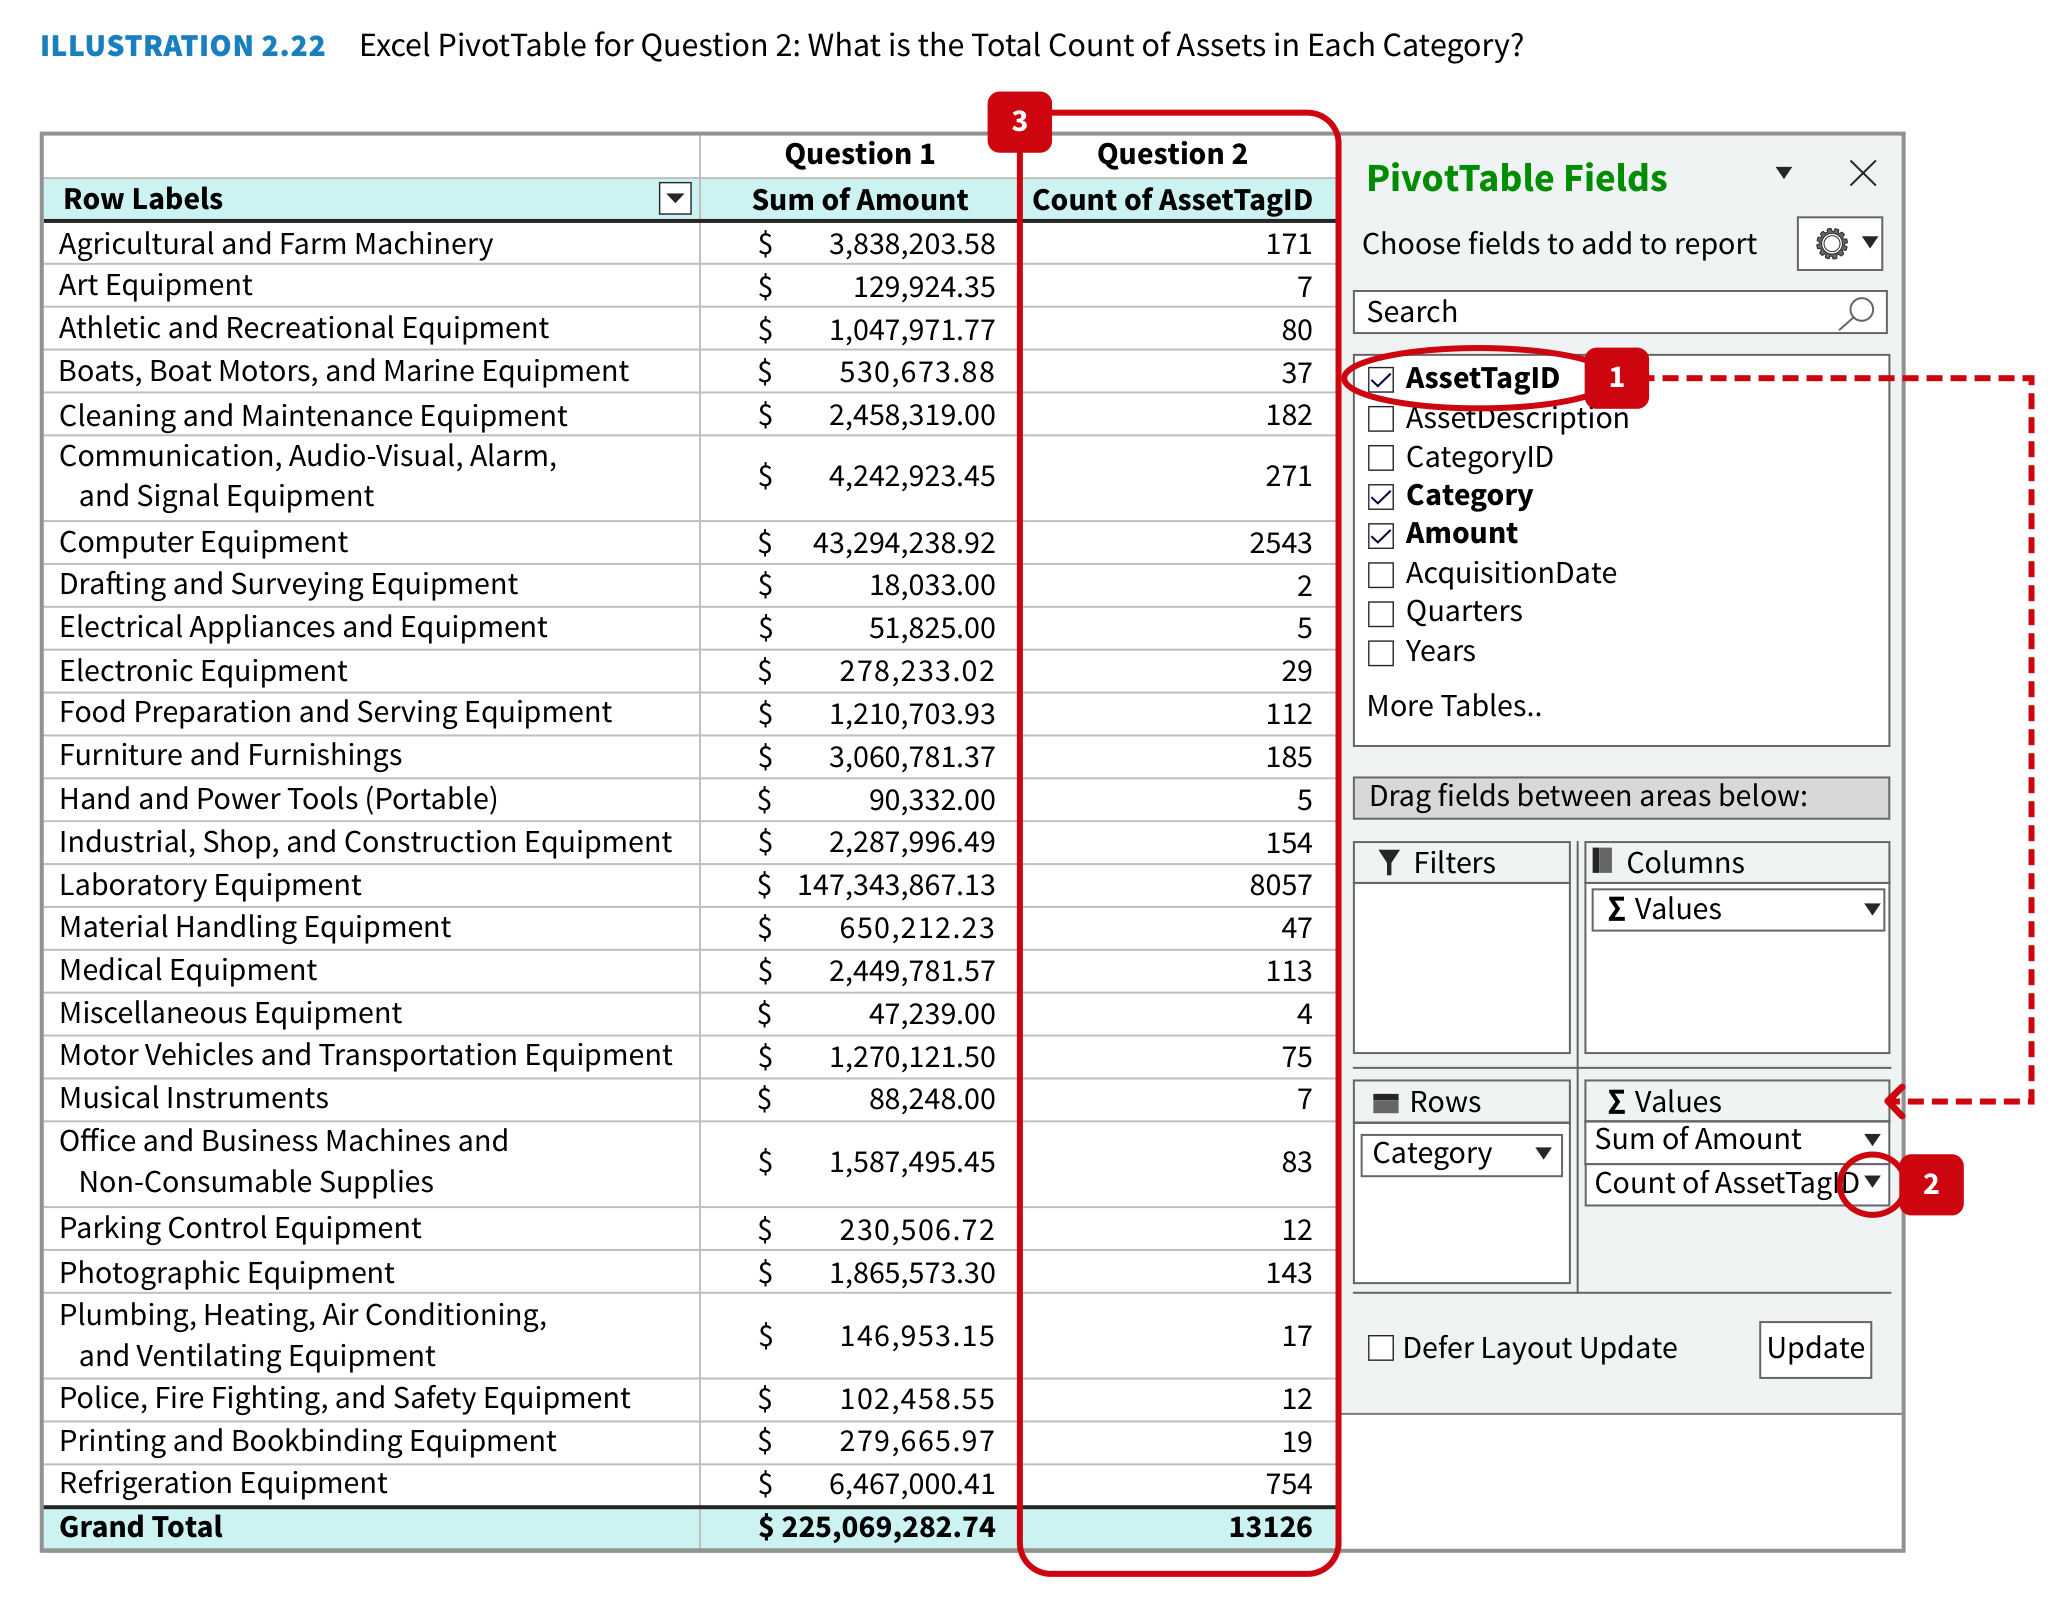
\includegraphics[height=0.65\textheight]{../textbookForPractice/Figures/Ch_02/ILLUSTRATION 2.22.png}
        \caption{Thay đổi hàm từ Sum thành Count để đếm số lượng tài sản.}
    \end{figure}
\end{frame}

\begin{frame}{Lọc Pivot Tables (Hộp Filter)}
    \begin{figure}[h]
        \centering
        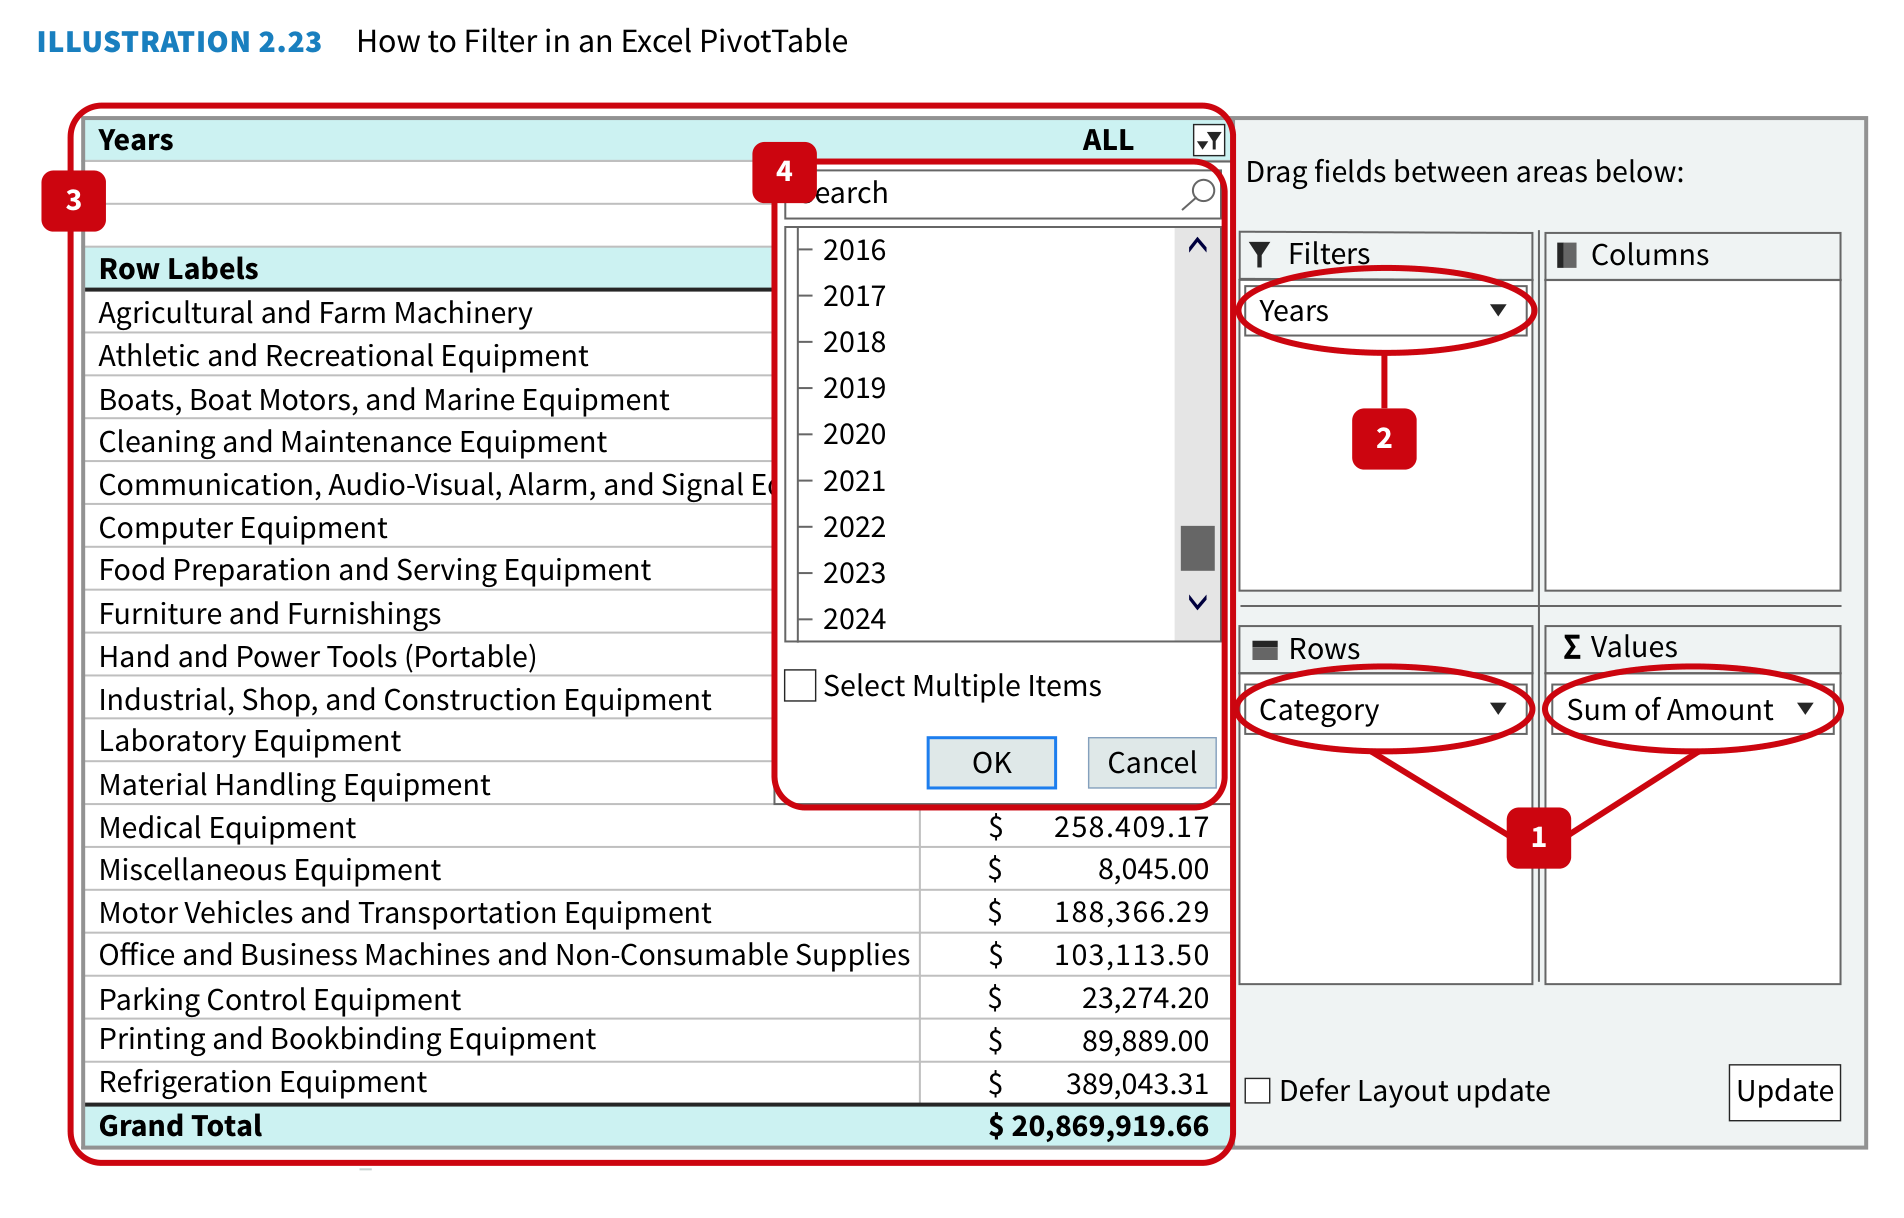
\includegraphics[height=0.6\textheight]{../textbookForPractice/Figures/Ch_02/ILLUSTRATION 2.23.png}
        \caption{Kéo trường Asset Sub-Category vào vùng Filters để tạo bộ lọc tổng.}
    \end{figure}
\end{frame}

\begin{frame}{Sử dụng Slicers để Lọc Trực quan}
    \begin{columns}
        \begin{column}{0.4\textwidth}
            \begin{figure}[h]
                \centering
                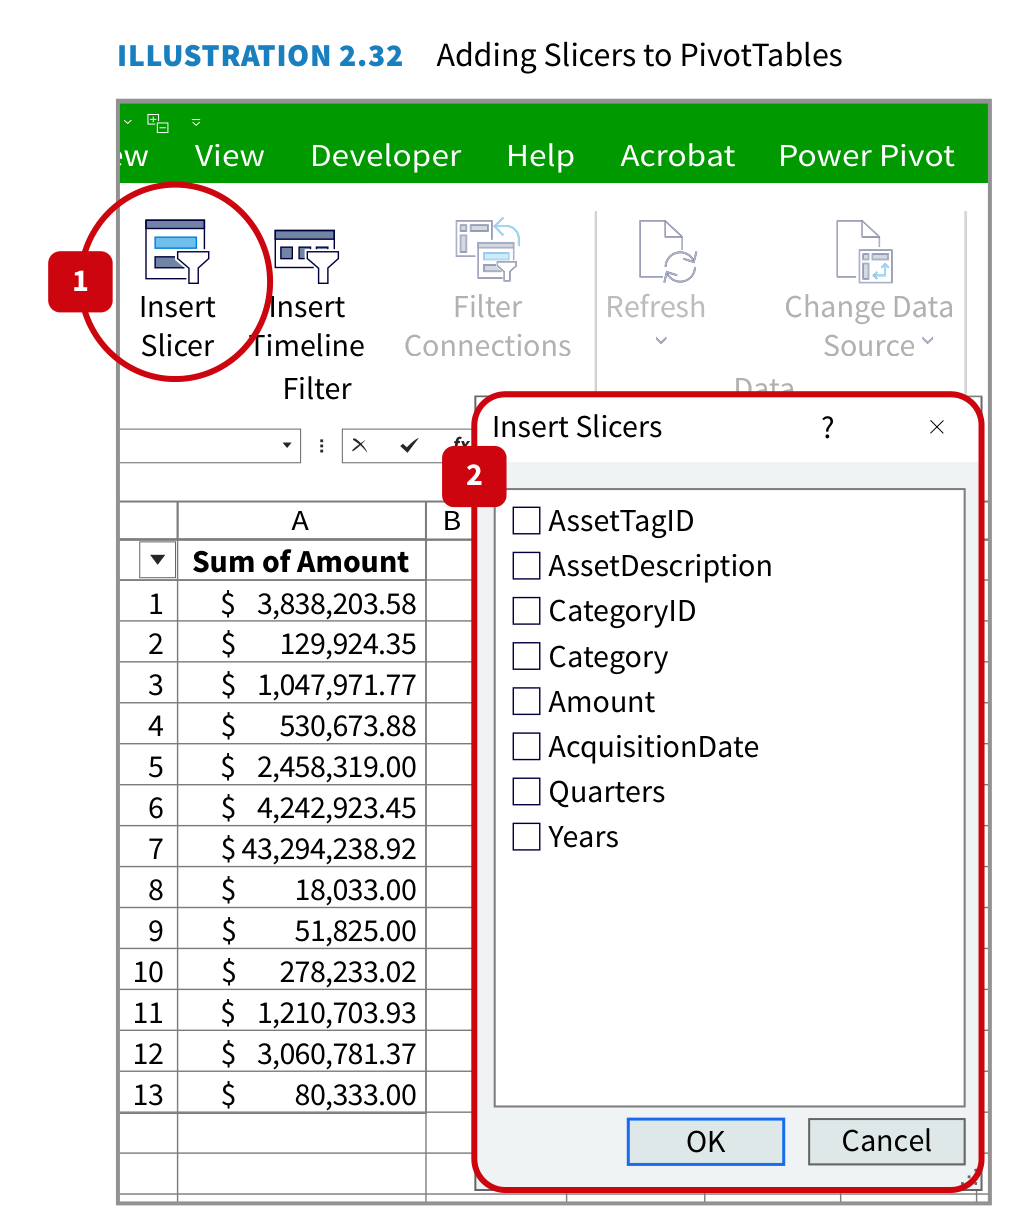
\includegraphics[width=\textwidth]{../textbookForPractice/Figures/Ch_02/ILLUSTRATION 2.32.png}
                \caption{Chèn Slicer từ menu Insert.}
            \end{figure}
        \end{column}
        \begin{column}{0.6\textwidth}
            \begin{figure}[h]
                \centering
                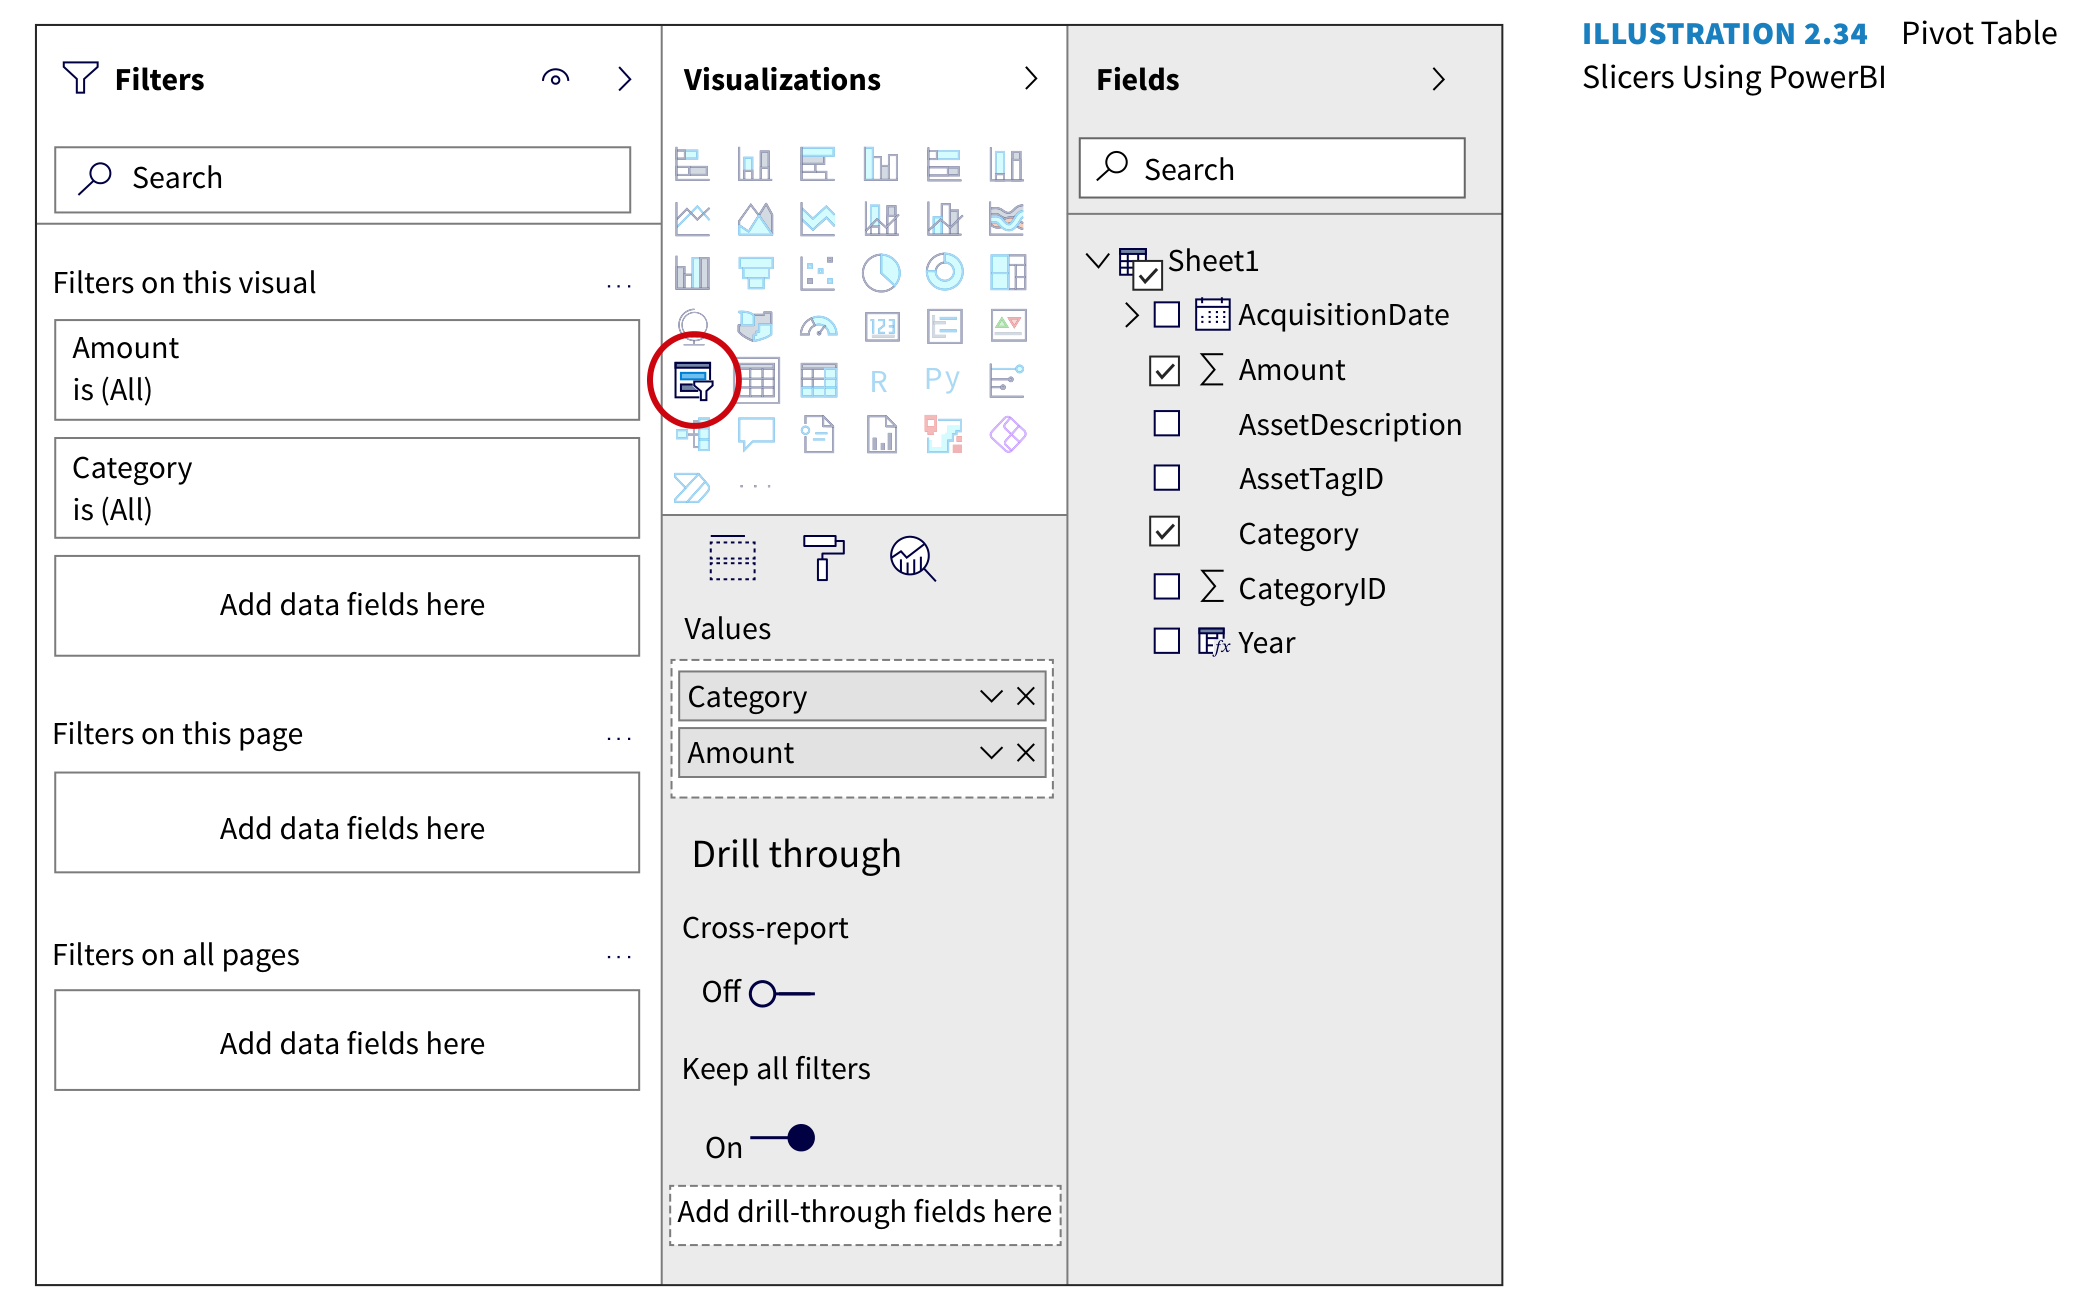
\includegraphics[width=\textwidth]{../textbookForPractice/Figures/Ch_02/ILLUSTRATION 2.34.png}
                \caption{Slicer tạo các nút bấm trực quan để lọc dữ liệu (vd: Lọc theo Name).}
            \end{figure}
        \end{column}
    \end{columns}
\end{frame}

\begin{frame}{Áp dụng (Apply It 2.3) - Phân tích Bán hàng bằng PivotTables}
    \begin{figure}[h]
        \centering
        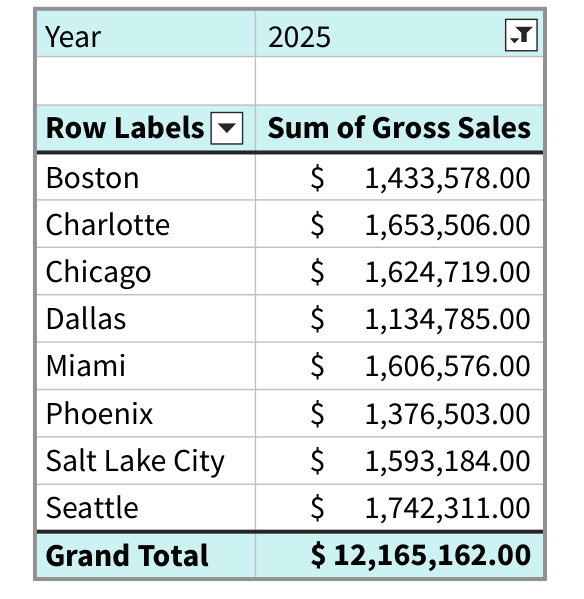
\includegraphics[height=0.65\textheight]{../textbookForPractice/Figures/Ch_02/Apply It 2.3_1.png}
        \caption{Tạo báo cáo doanh số theo tháng và sản phẩm.}
    \end{figure}
\end{frame}

% --- Phần 4: Các Thước Đo Mô Tả (LO 2.4) ---
\begin{frame}{2.4 Thước Đo Mô Tả Giúp Hiểu Dữ Liệu}
    \begin{itemize}
        \item Thống kê mô tả được sử dụng trong giai đoạn \textbf{Khám phá Dữ liệu} (Giai đoạn 2).
        \item 3 nhóm thước đo chính:
        \begin{itemize}
            \item \textbf{Vị trí trung tâm (Location/Central Tendency):} Mean (Trung bình), Median (Trung vị), Mode (Yếu vị).
            \item \textbf{Độ phân tán (Dispersion):} Range (Khoảng), Variance (Phương sai), Standard Deviation (Độ lệch chuẩn).
            \item \textbf{Hình dạng (Shape):} Skewness (Độ lệch), Kurtosis (Độ nhọn).
        \end{itemize}
    \end{itemize}
\end{frame}

\begin{frame}{Tính toán Các Thước đo Vị trí (Mean, Median, Mode)}
    \begin{figure}[h]
        \centering
        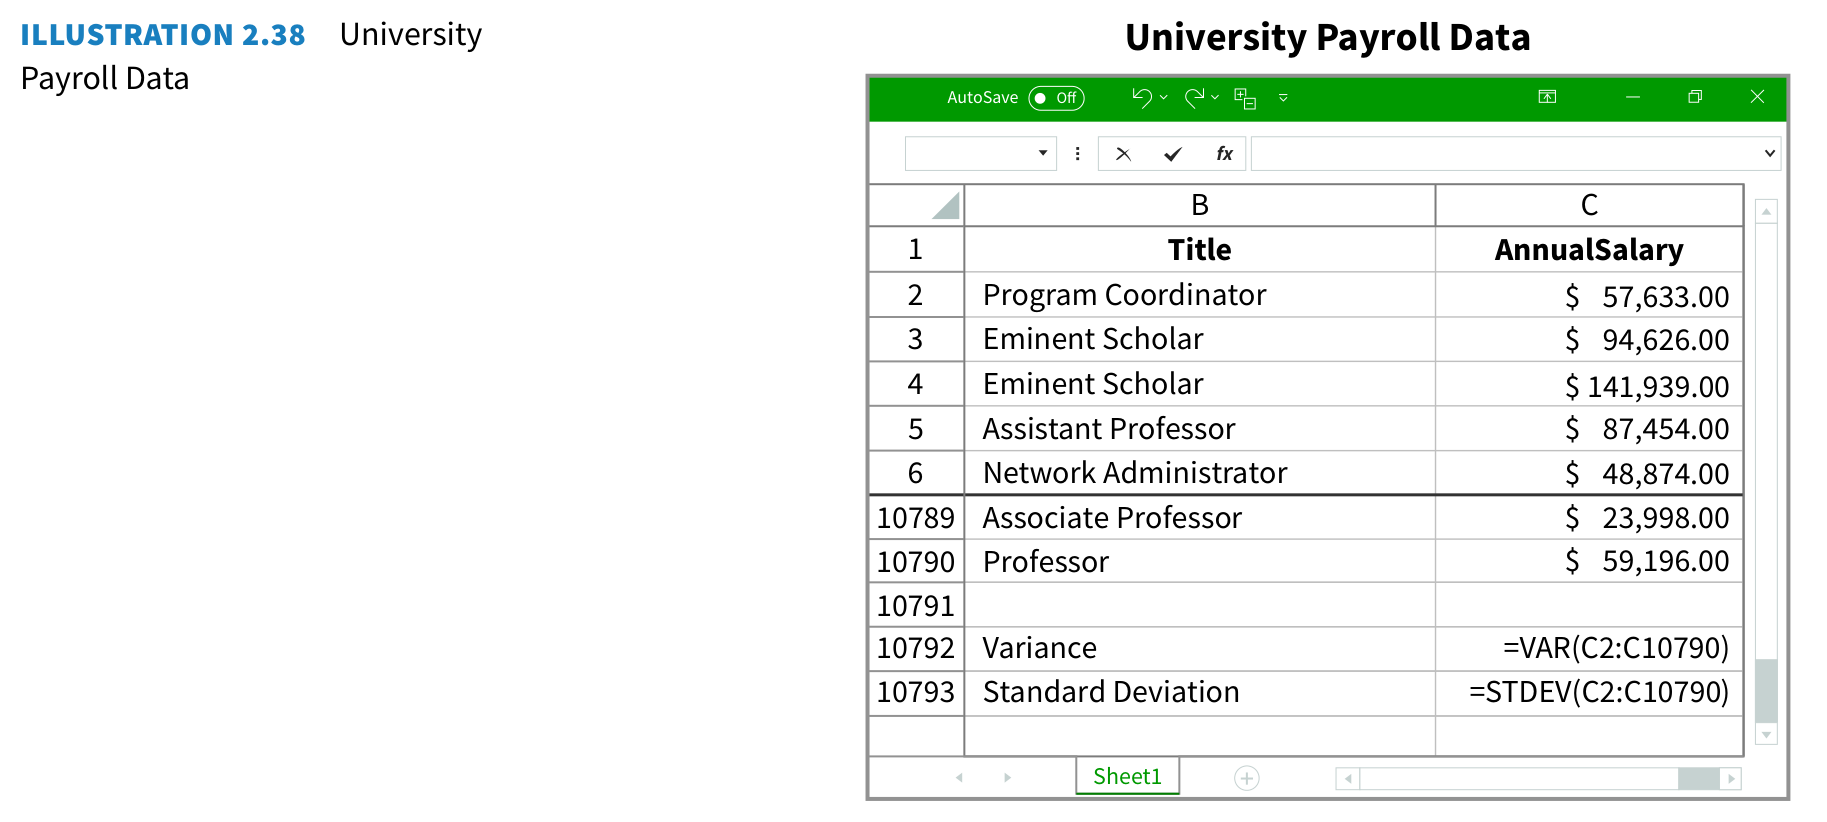
\includegraphics[height=0.65\textheight]{../textbookForPractice/Figures/Ch_02/ILLUSTRATION 2.38.png}
        \caption{Sử dụng hàm AVERAGE, MEDIAN, MODE.SNGL trong Excel.}
    \end{figure}
\end{frame}

\begin{frame}{Các thước đo Hình dạng (Skewness)}
    \begin{figure}[h]
        \centering
        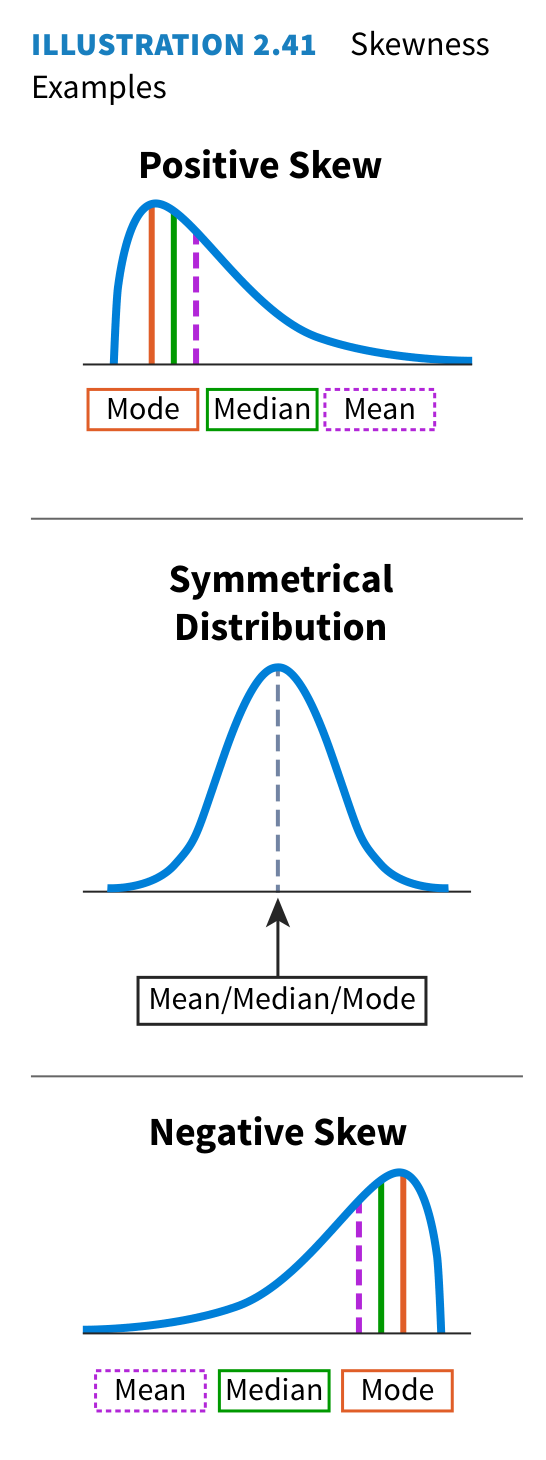
\includegraphics[height=0.55\textheight]{../textbookForPractice/Figures/Ch_02/ILLUSTRATION 2.41.png}
        \caption{Phân phối lệch trái (Left-Skewed) và lệch phải (Right-Skewed).}
    \end{figure}
\end{frame}

\begin{frame}{Biểu đồ Tần suất (Histograms)}
    \begin{columns}
        \begin{column}{0.5\textwidth}
            \begin{figure}[h]
                \centering
                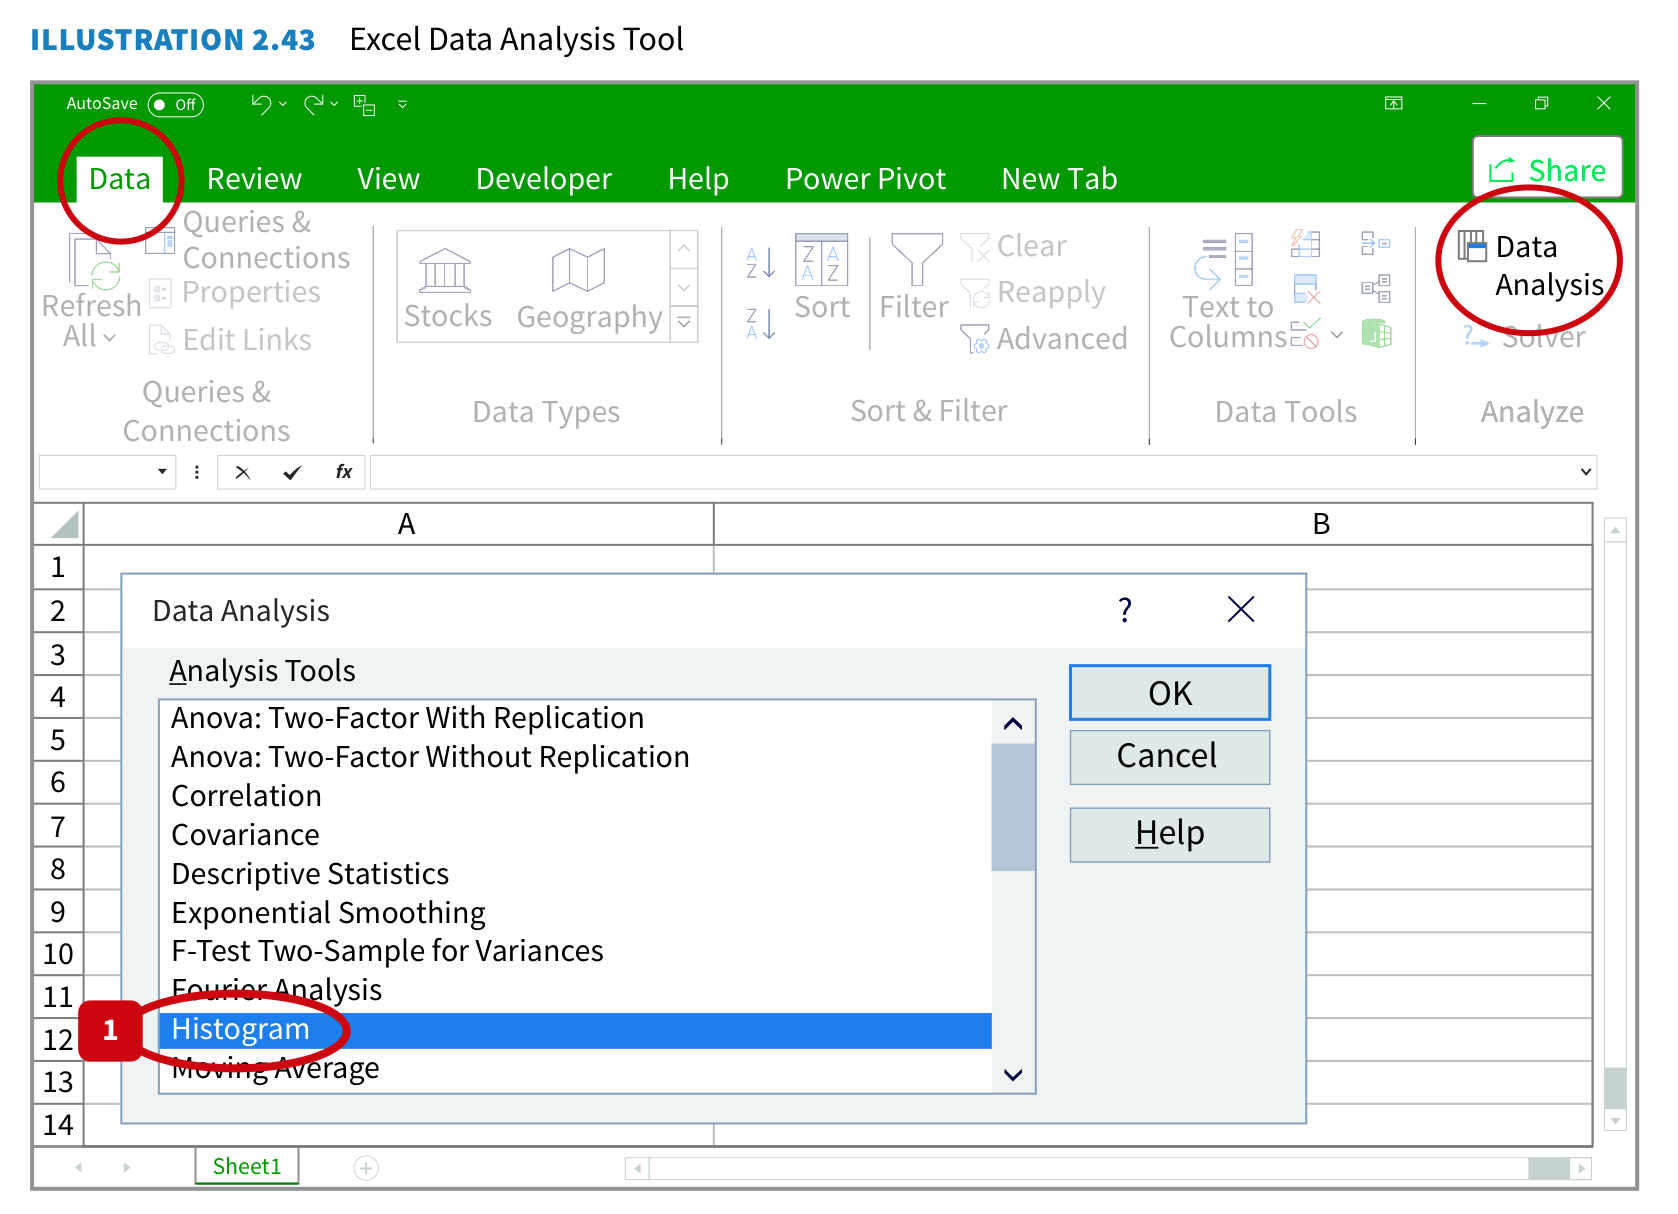
\includegraphics[width=\textwidth]{../textbookForPractice/Figures/Ch_02/ILLUSTRATION 2.43.png}
                \caption{Xây dựng bảng phân phối tần số (Bins).}
            \end{figure}
        \end{column}
        \begin{column}{0.5\textwidth}
            \begin{figure}[h]
                \centering
                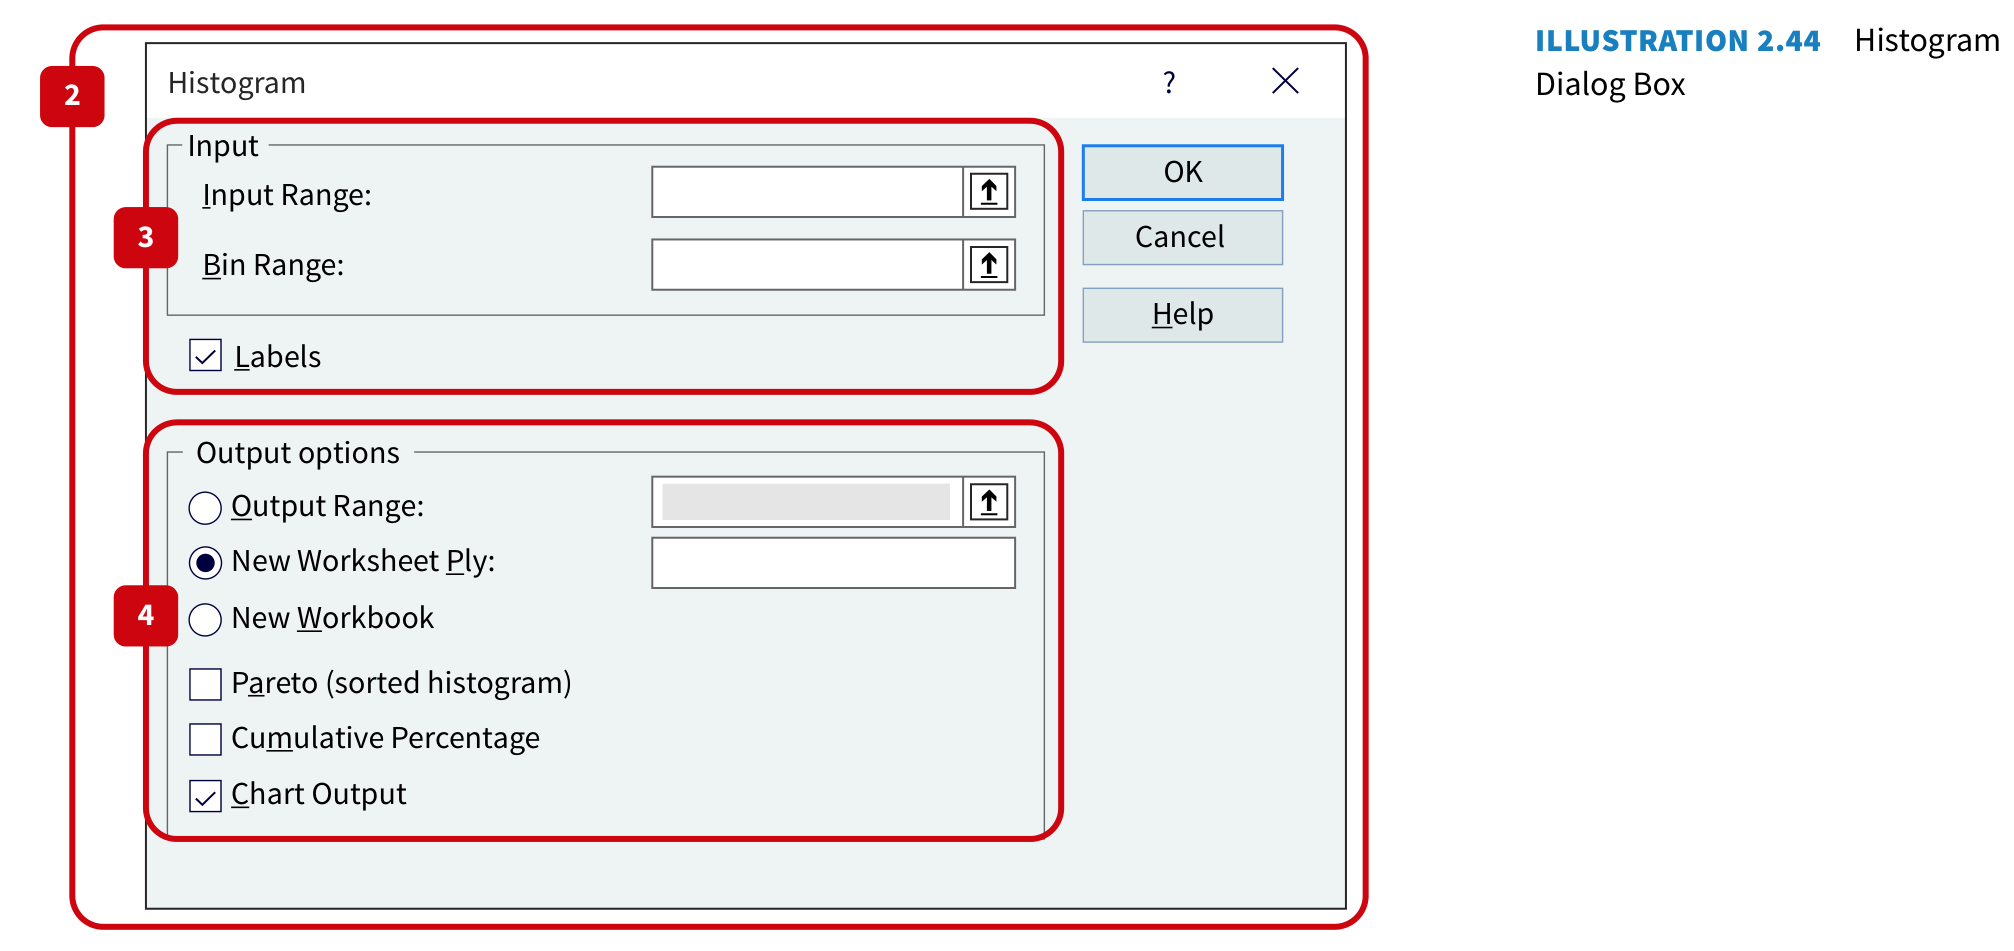
\includegraphics[width=\textwidth]{../textbookForPractice/Figures/Ch_02/ILLUSTRATION 2.44.png}
                \caption{Trực quan hóa bằng Histogram.}
            \end{figure}
        \end{column}
    \end{columns}
\end{frame}

\begin{frame}{Các Công cụ Thống kê Mô tả Excel (Data Analysis Toolpak)}
    \begin{figure}[h]
        \centering
        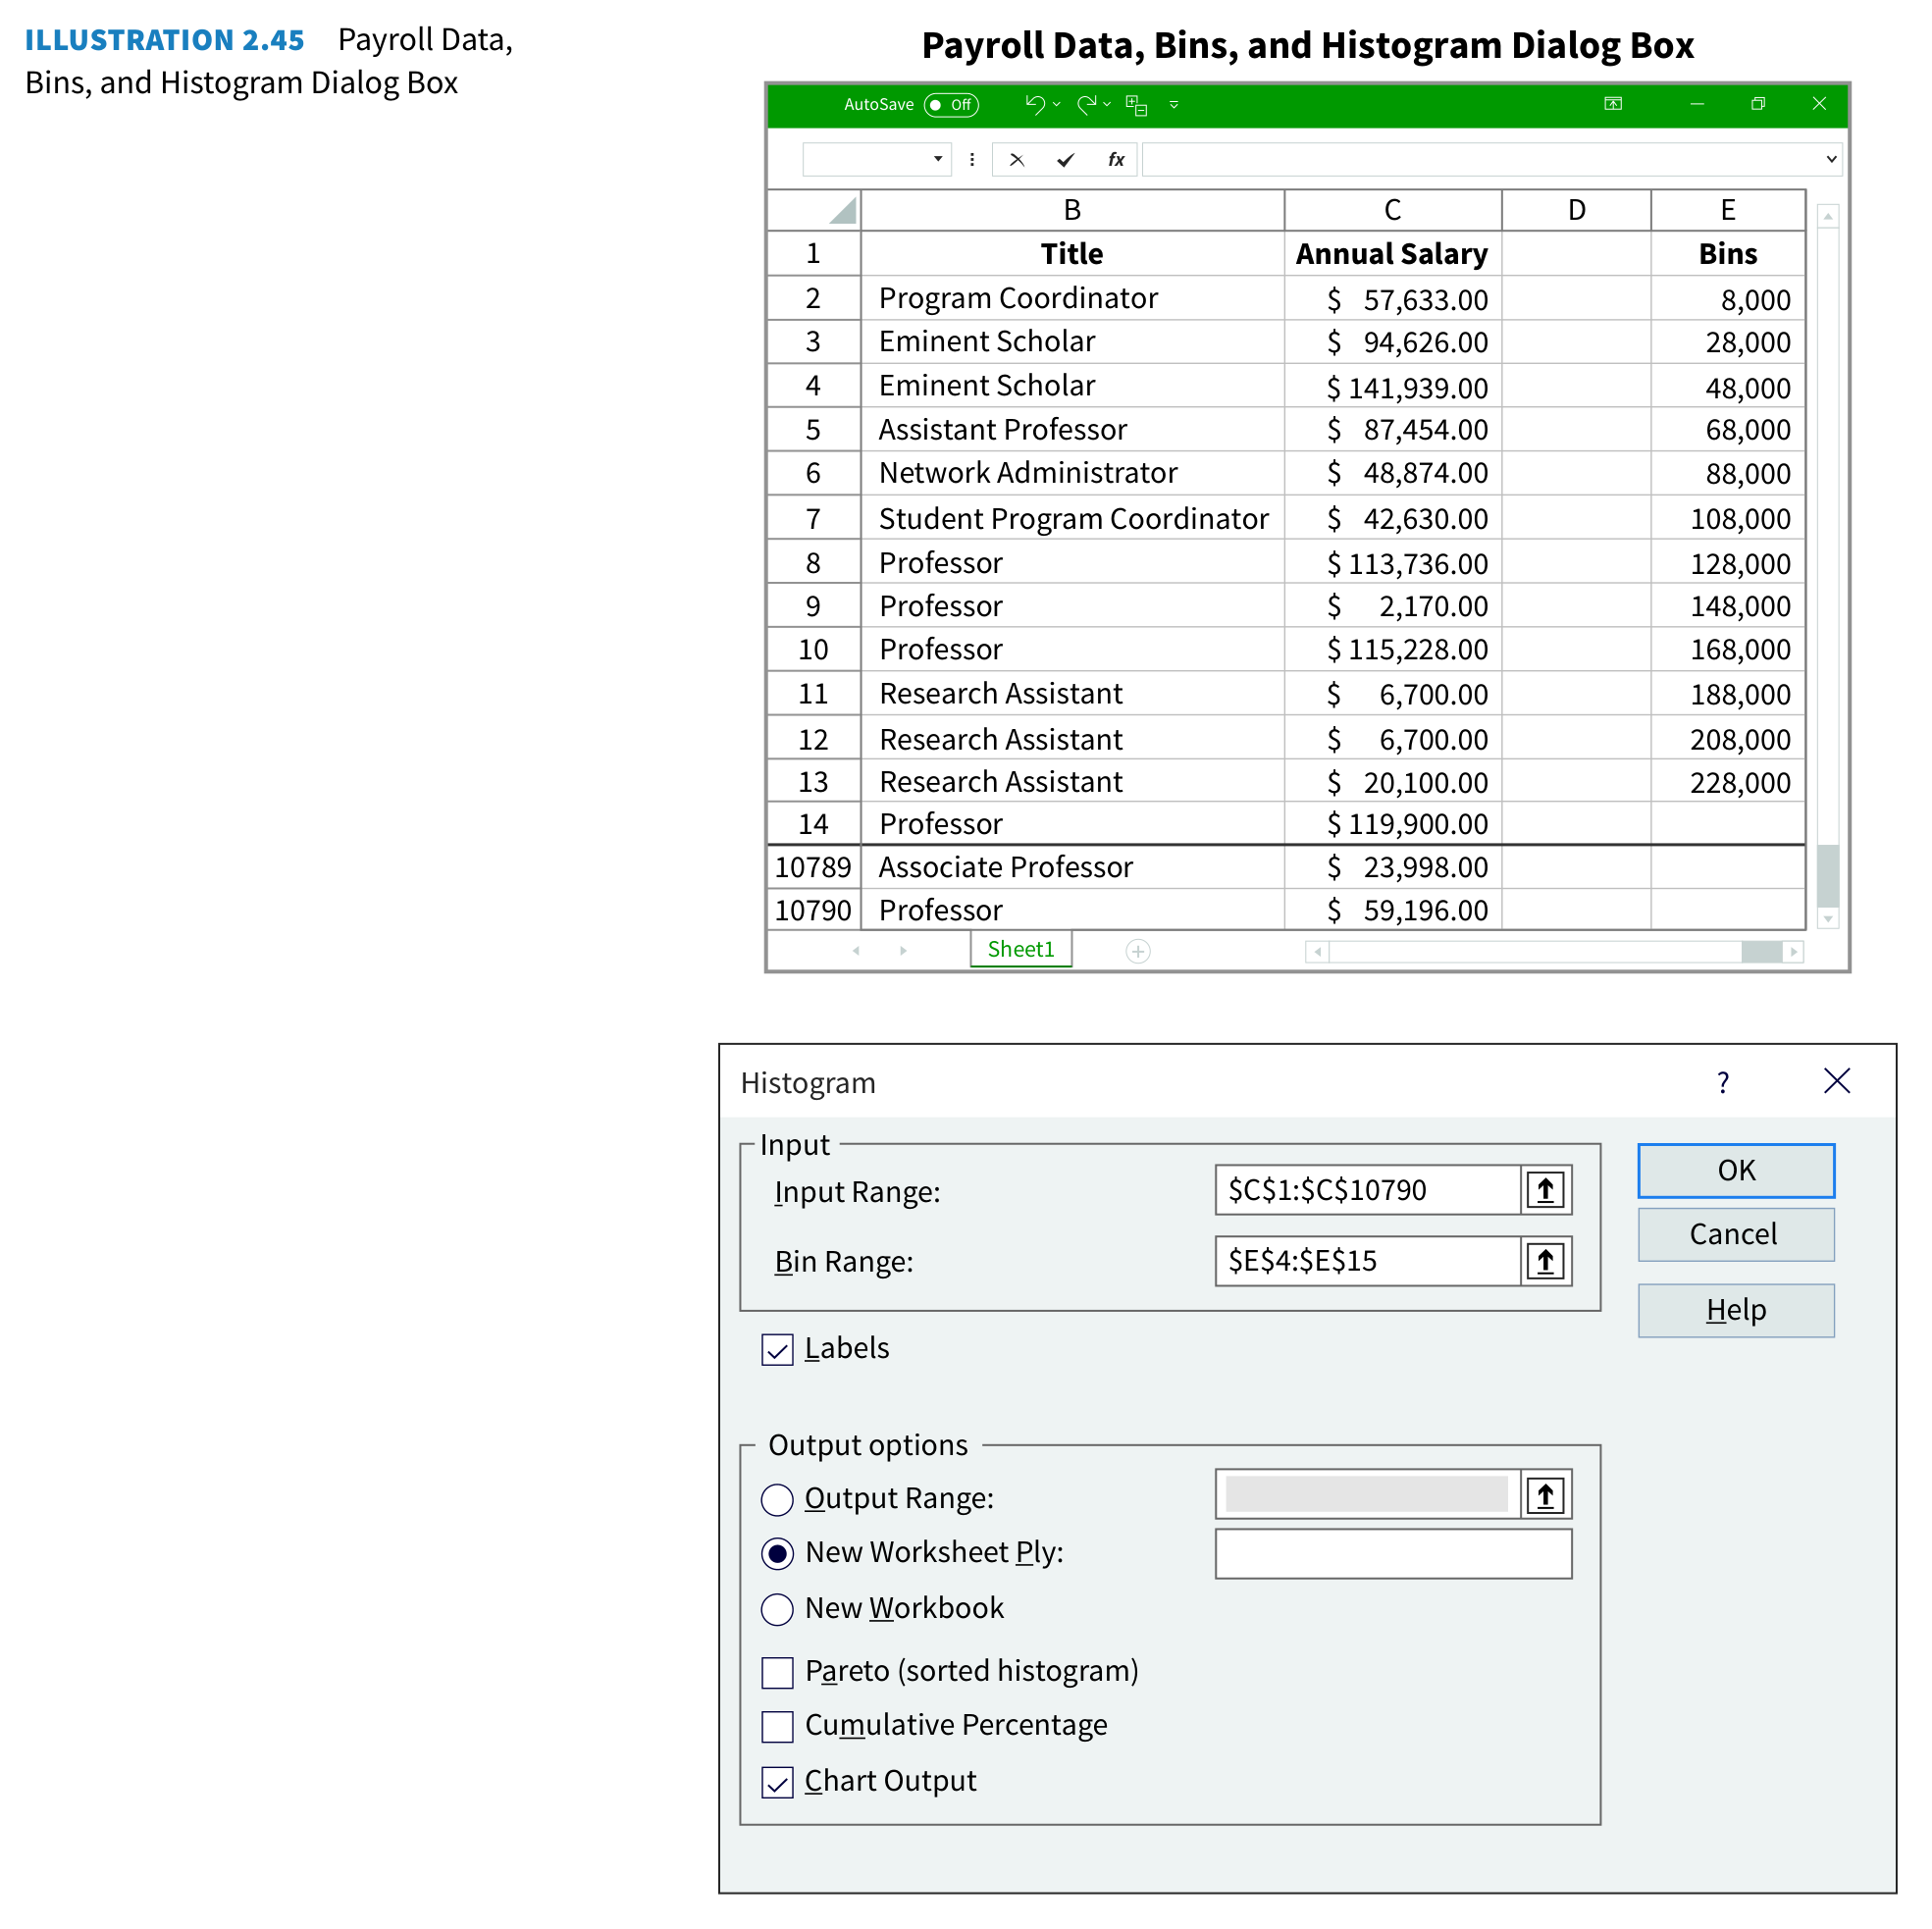
\includegraphics[height=0.65\textheight]{../textbookForPractice/Figures/Ch_02/ILLUSTRATION 2.45.png}
        \caption{Tự động xuất toàn bộ các chỉ số thống kê cơ bản trong 1 cú nhấp chuột.}
    \end{figure}
\end{frame}

\begin{frame}{Phân tích Tương quan (Correlation Analysis)}
    \begin{figure}[h]
        \centering
        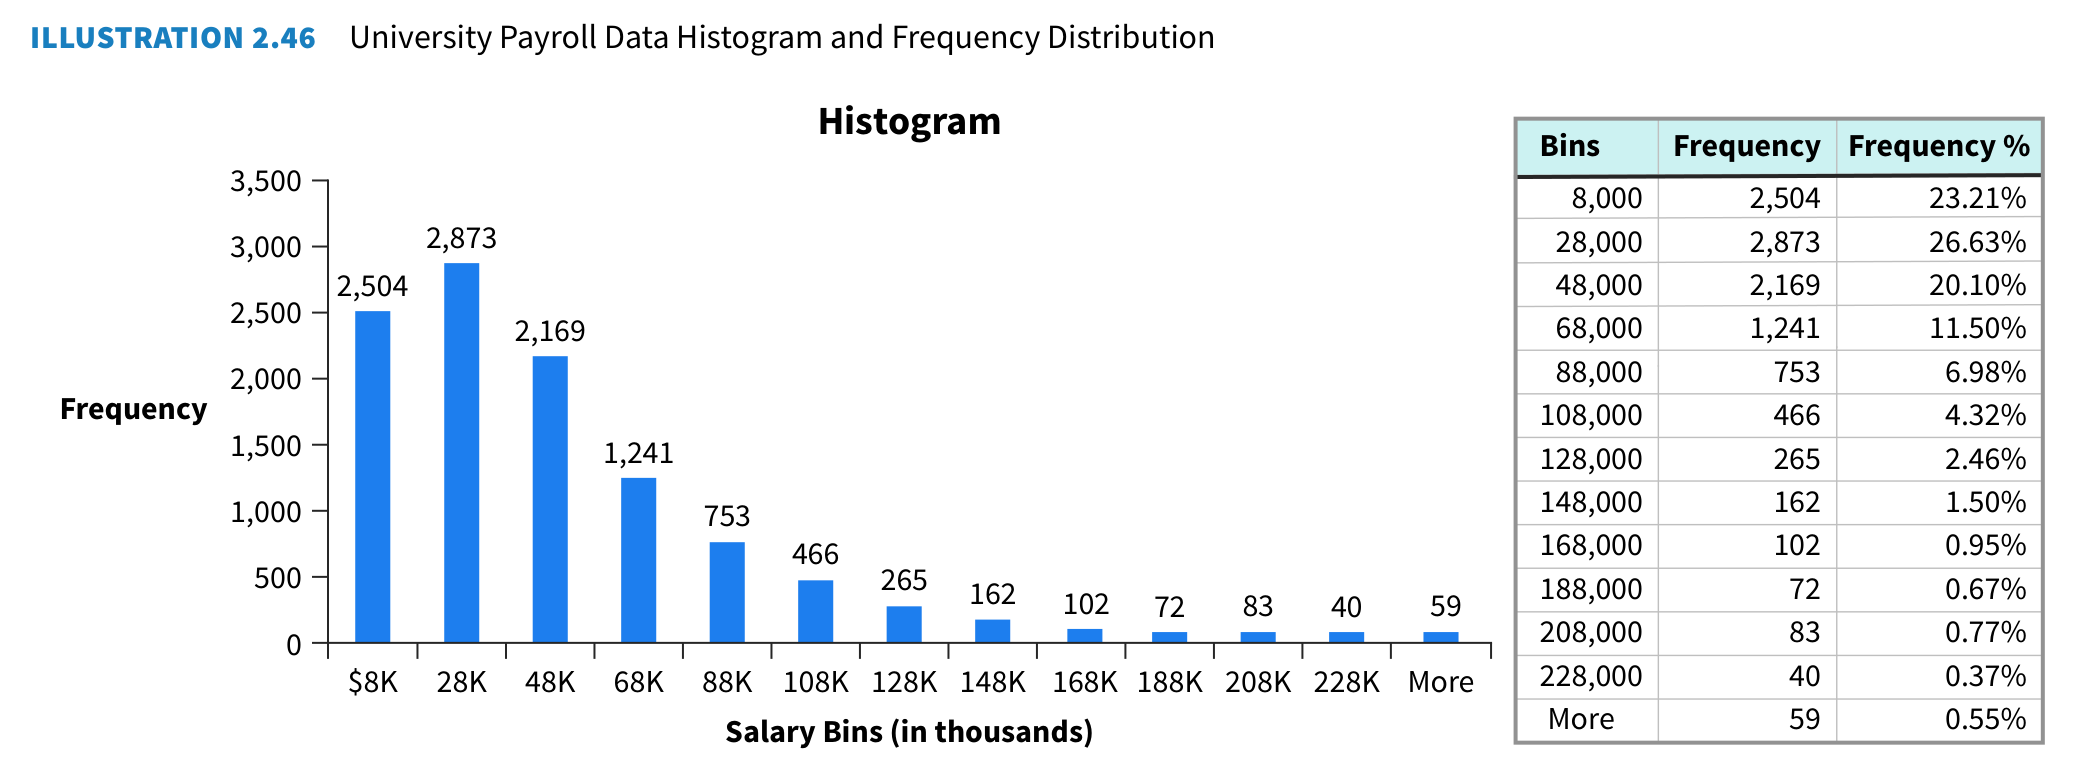
\includegraphics[height=0.55\textheight]{../textbookForPractice/Figures/Ch_02/ILLUSTRATION 2.46.png}
        \caption{Hệ số tương quan (r) đo lường mức độ liên hệ giữa 2 biến liên tục (từ -1 đến 1).}
    \end{figure}
\end{frame}

\begin{frame}{Thực hiện Phân tích Tương quan bằng Excel}
    \begin{figure}[h]
        \centering
        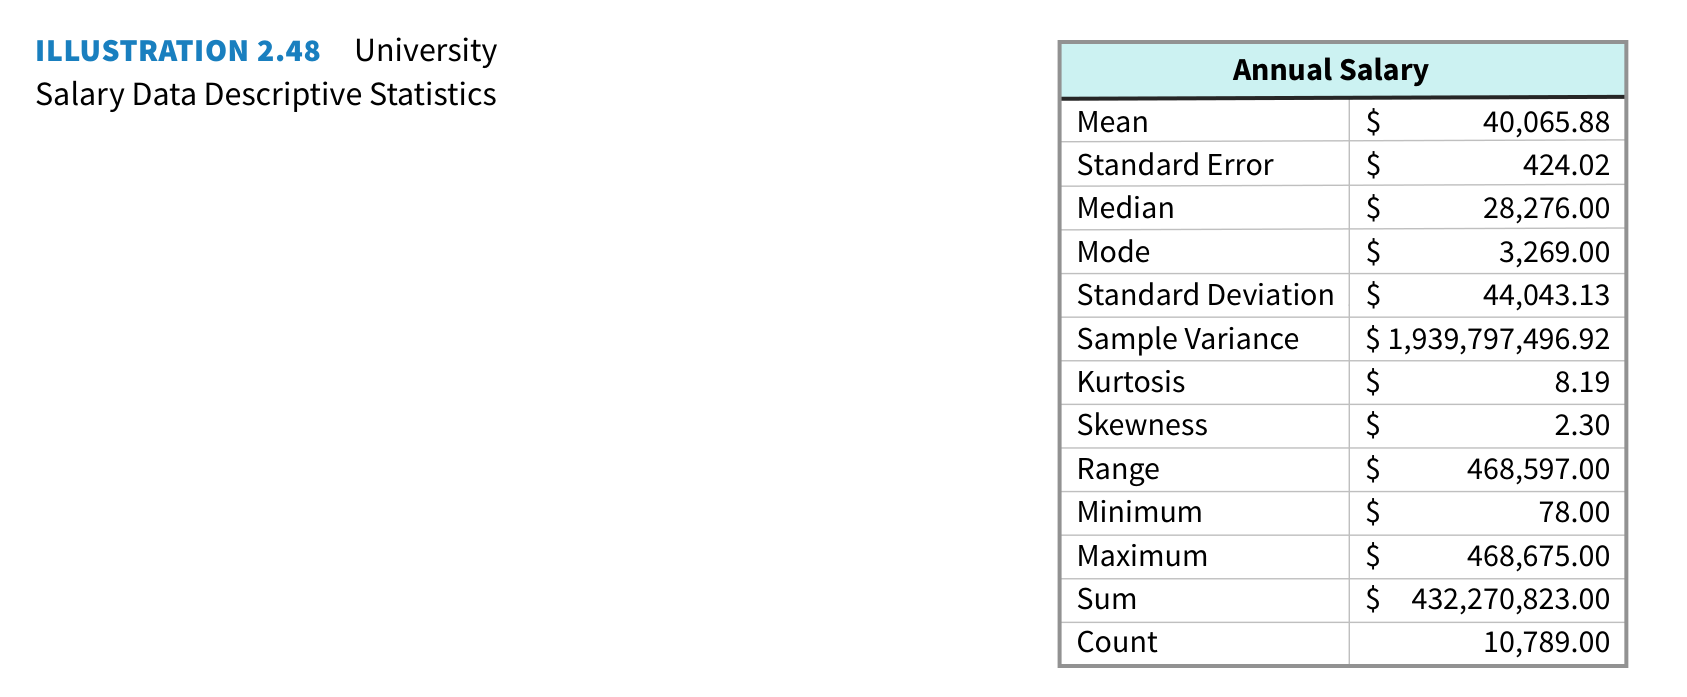
\includegraphics[height=0.55\textheight]{../textbookForPractice/Figures/Ch_02/ILLUSTRATION 2.48.png}
        \caption{Sử dụng Ma trận tương quan (Correlation Matrix) từ Data Analysis Toolpak.}
    \end{figure}
\end{frame}

\begin{frame}{Áp dụng (Apply It 2.4) - Kiểm toán Chi phí Bảo hành}
    \begin{figure}[h]
        \centering
        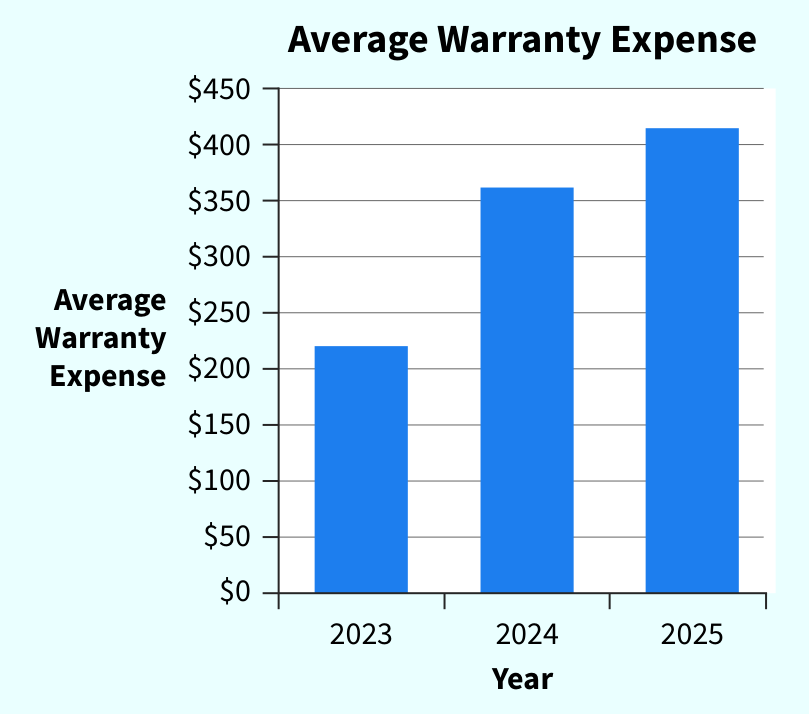
\includegraphics[height=0.65\textheight]{../textbookForPractice/Figures/Ch_02/Apply It 2.4_1.png}
        \caption{Phân tích độ lệch chuẩn và histogram để phát hiện chi phí bảo hành bất thường.}
    \end{figure}
\end{frame}

% --- Phần 5: Trực quan hóa Dữ Liệu (LO 2.5) ---
\begin{frame}{2.5 Trực quan hóa Được Sử dụng Như thế nào?}
    \begin{itemize}
        \item Bộ não con người xử lý hình ảnh nhanh hơn 60.000 lần so với văn bản.
        \item Trực quan hóa giúp nhận diện các điểm dị biệt (outliers) và xu hướng (trends) không thể thấy trong các bảng số liệu.
        \item \textbf{Nguyên tắc:} "Bức tranh đáng giá ngàn con số".
    \end{itemize}
\end{frame}

\begin{frame}{Lợi ích của Trực quan hóa so với Bảng số liệu}
    \begin{columns}
        \begin{column}{0.5\textwidth}
            \begin{figure}[h]
                \centering
                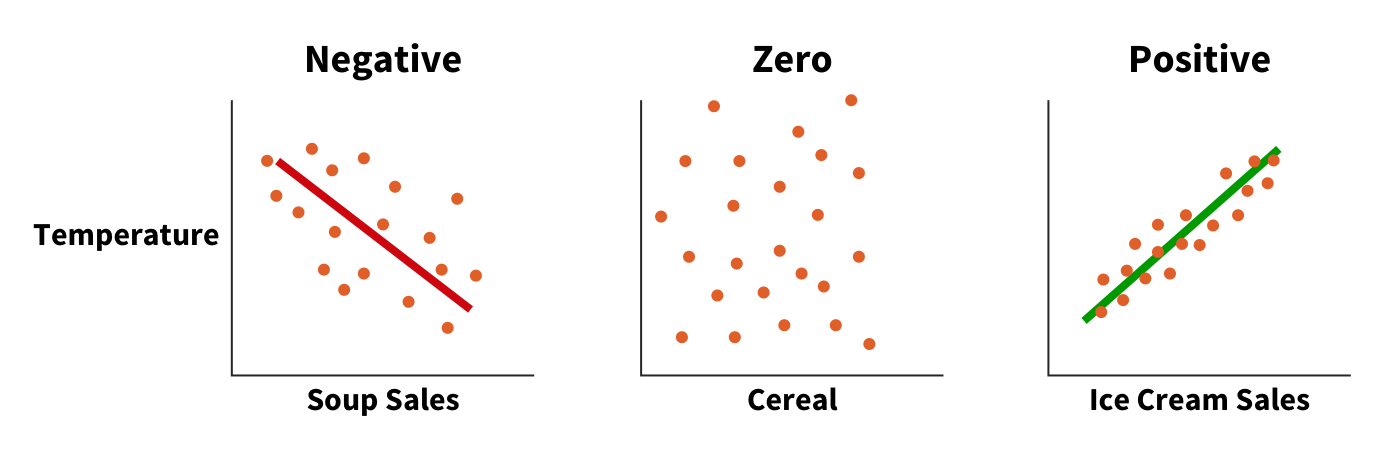
\includegraphics[width=\textwidth]{../textbookForPractice/Figures/Ch_02/ILLUSTRATION 2.49.png}
                \caption{Nhìn bảng số liệu khó phát hiện xu hướng.}
            \end{figure}
        \end{column}
        \begin{column}{0.5\textwidth}
            \begin{figure}[h]
                \centering
                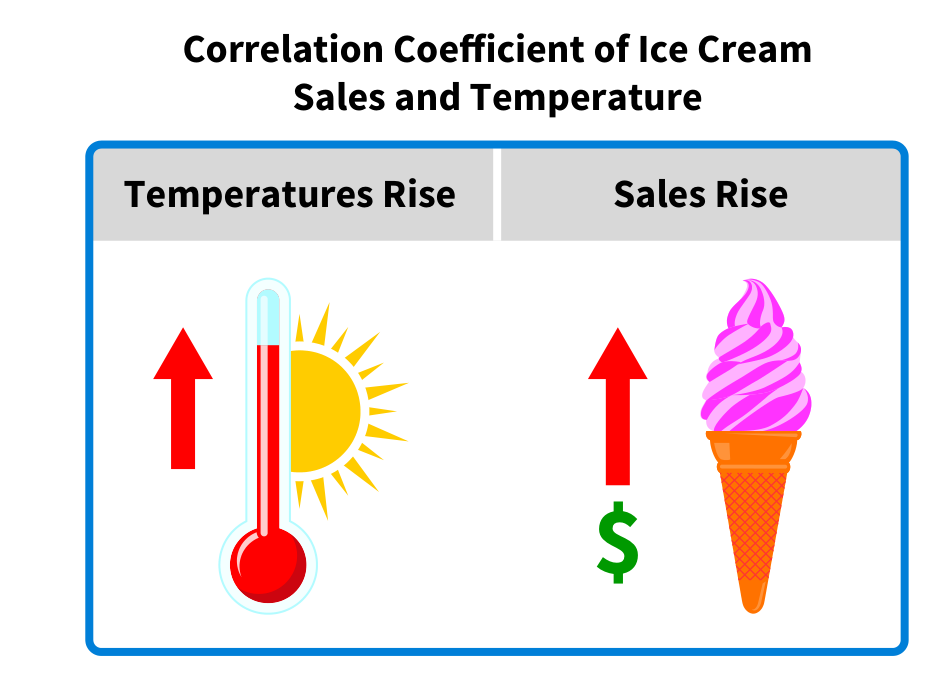
\includegraphics[width=\textwidth]{../textbookForPractice/Figures/Ch_02/ILLUSTRATION 2.51.png}
                \caption{Biểu đồ đường (Line Chart) lập tức cho thấy sự sụt giảm doanh số ở một số vùng.}
            \end{figure}
        \end{column}
    \end{columns}
\end{frame}

\begin{frame}{Lựa chọn Dạng Trực quan hóa (Decision Tree)}
    \begin{figure}[h]
        \centering
        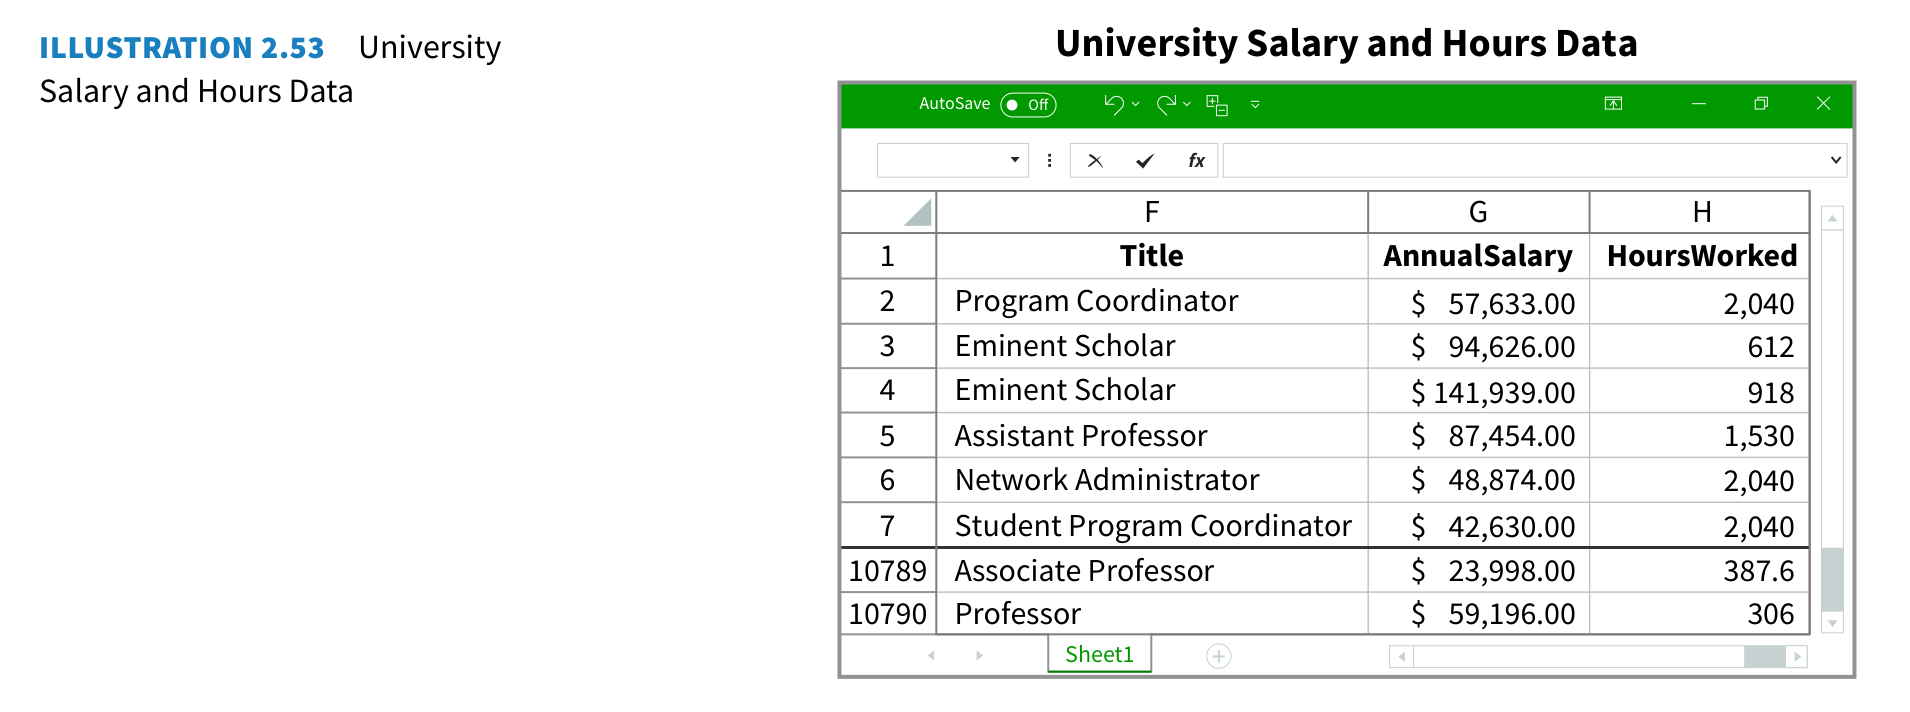
\includegraphics[height=0.65\textheight]{../textbookForPractice/Figures/Ch_02/ILLUSTRATION 2.53.png}
        \caption{Cây quyết định để chọn biểu đồ: So sánh, Thành phần, Phân phối, hay Tương quan?}
    \end{figure}
\end{frame}

\begin{frame}{Các Dạng Biểu đồ Phổ biến trong Excel (1/2)}
    \begin{columns}
        \begin{column}{0.5\textwidth}
            \begin{figure}[h]
                \centering
                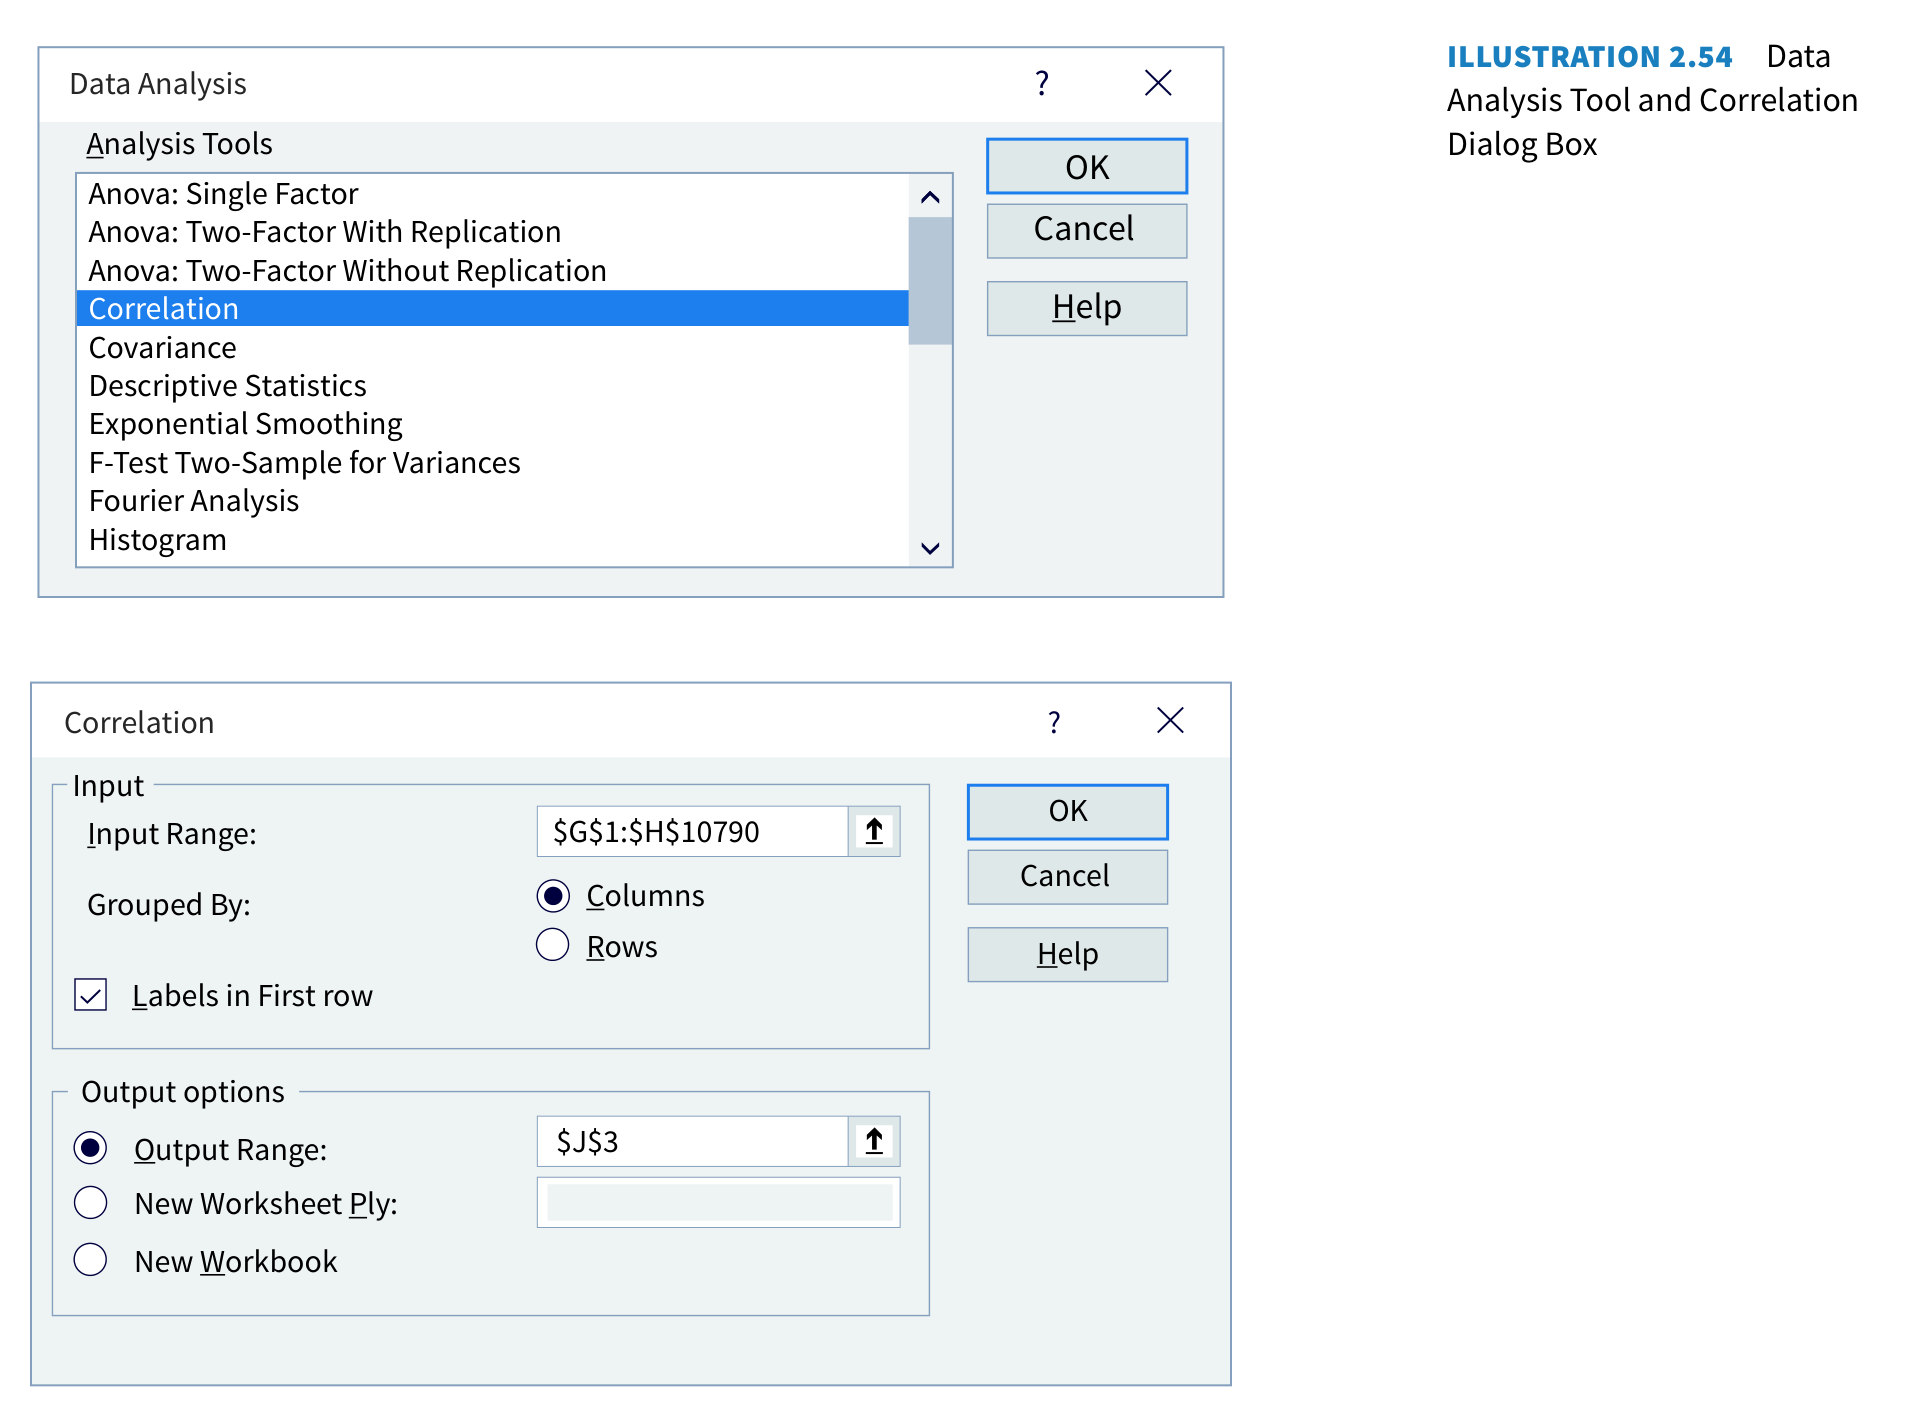
\includegraphics[width=\textwidth]{../textbookForPractice/Figures/Ch_02/ILLUSTRATION 2.54.png}
                \caption{Biểu đồ Cột (Column) \& Thanh (Bar).}
            \end{figure}
        \end{column}
        \begin{column}{0.5\textwidth}
            \begin{figure}[h]
                \centering
                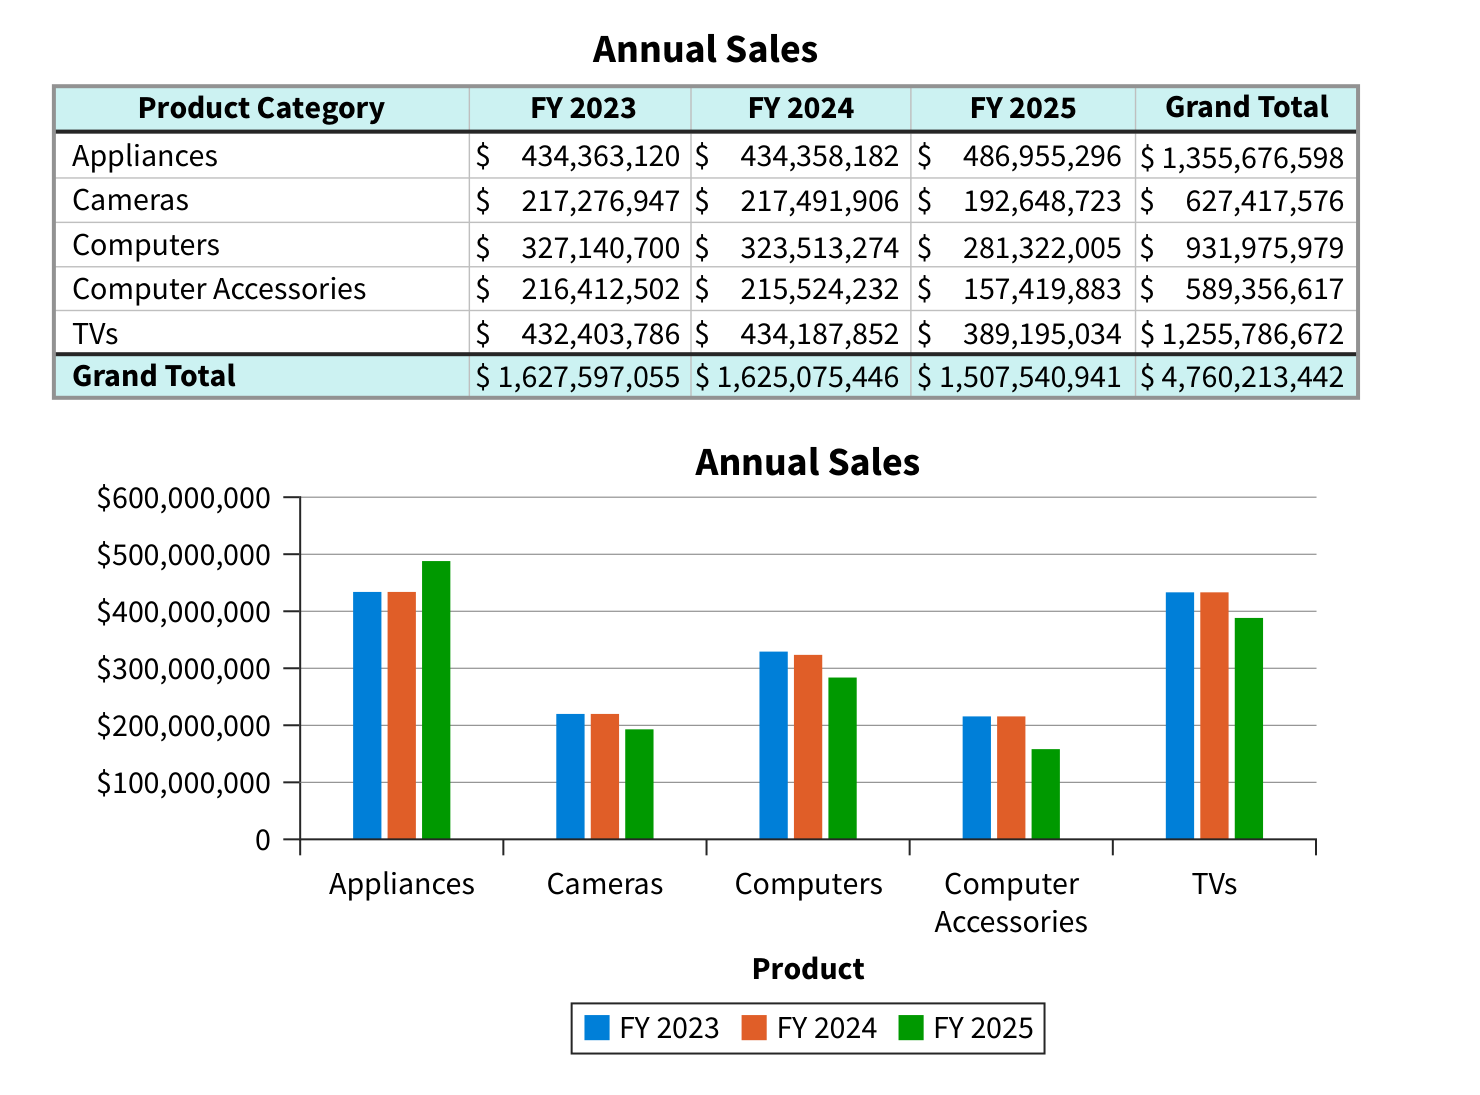
\includegraphics[width=\textwidth]{../textbookForPractice/Figures/Ch_02/ILLUSTRATION 2.56.png}
                \caption{Biểu đồ Phân tán (Scatter).}
            \end{figure}
        \end{column}
    \end{columns}
\end{frame}

\begin{frame}{Các Dạng Biểu đồ Phổ biến trong Excel (2/2)}
    \begin{columns}
        \begin{column}{0.5\textwidth}
            \begin{figure}[h]
                \centering
                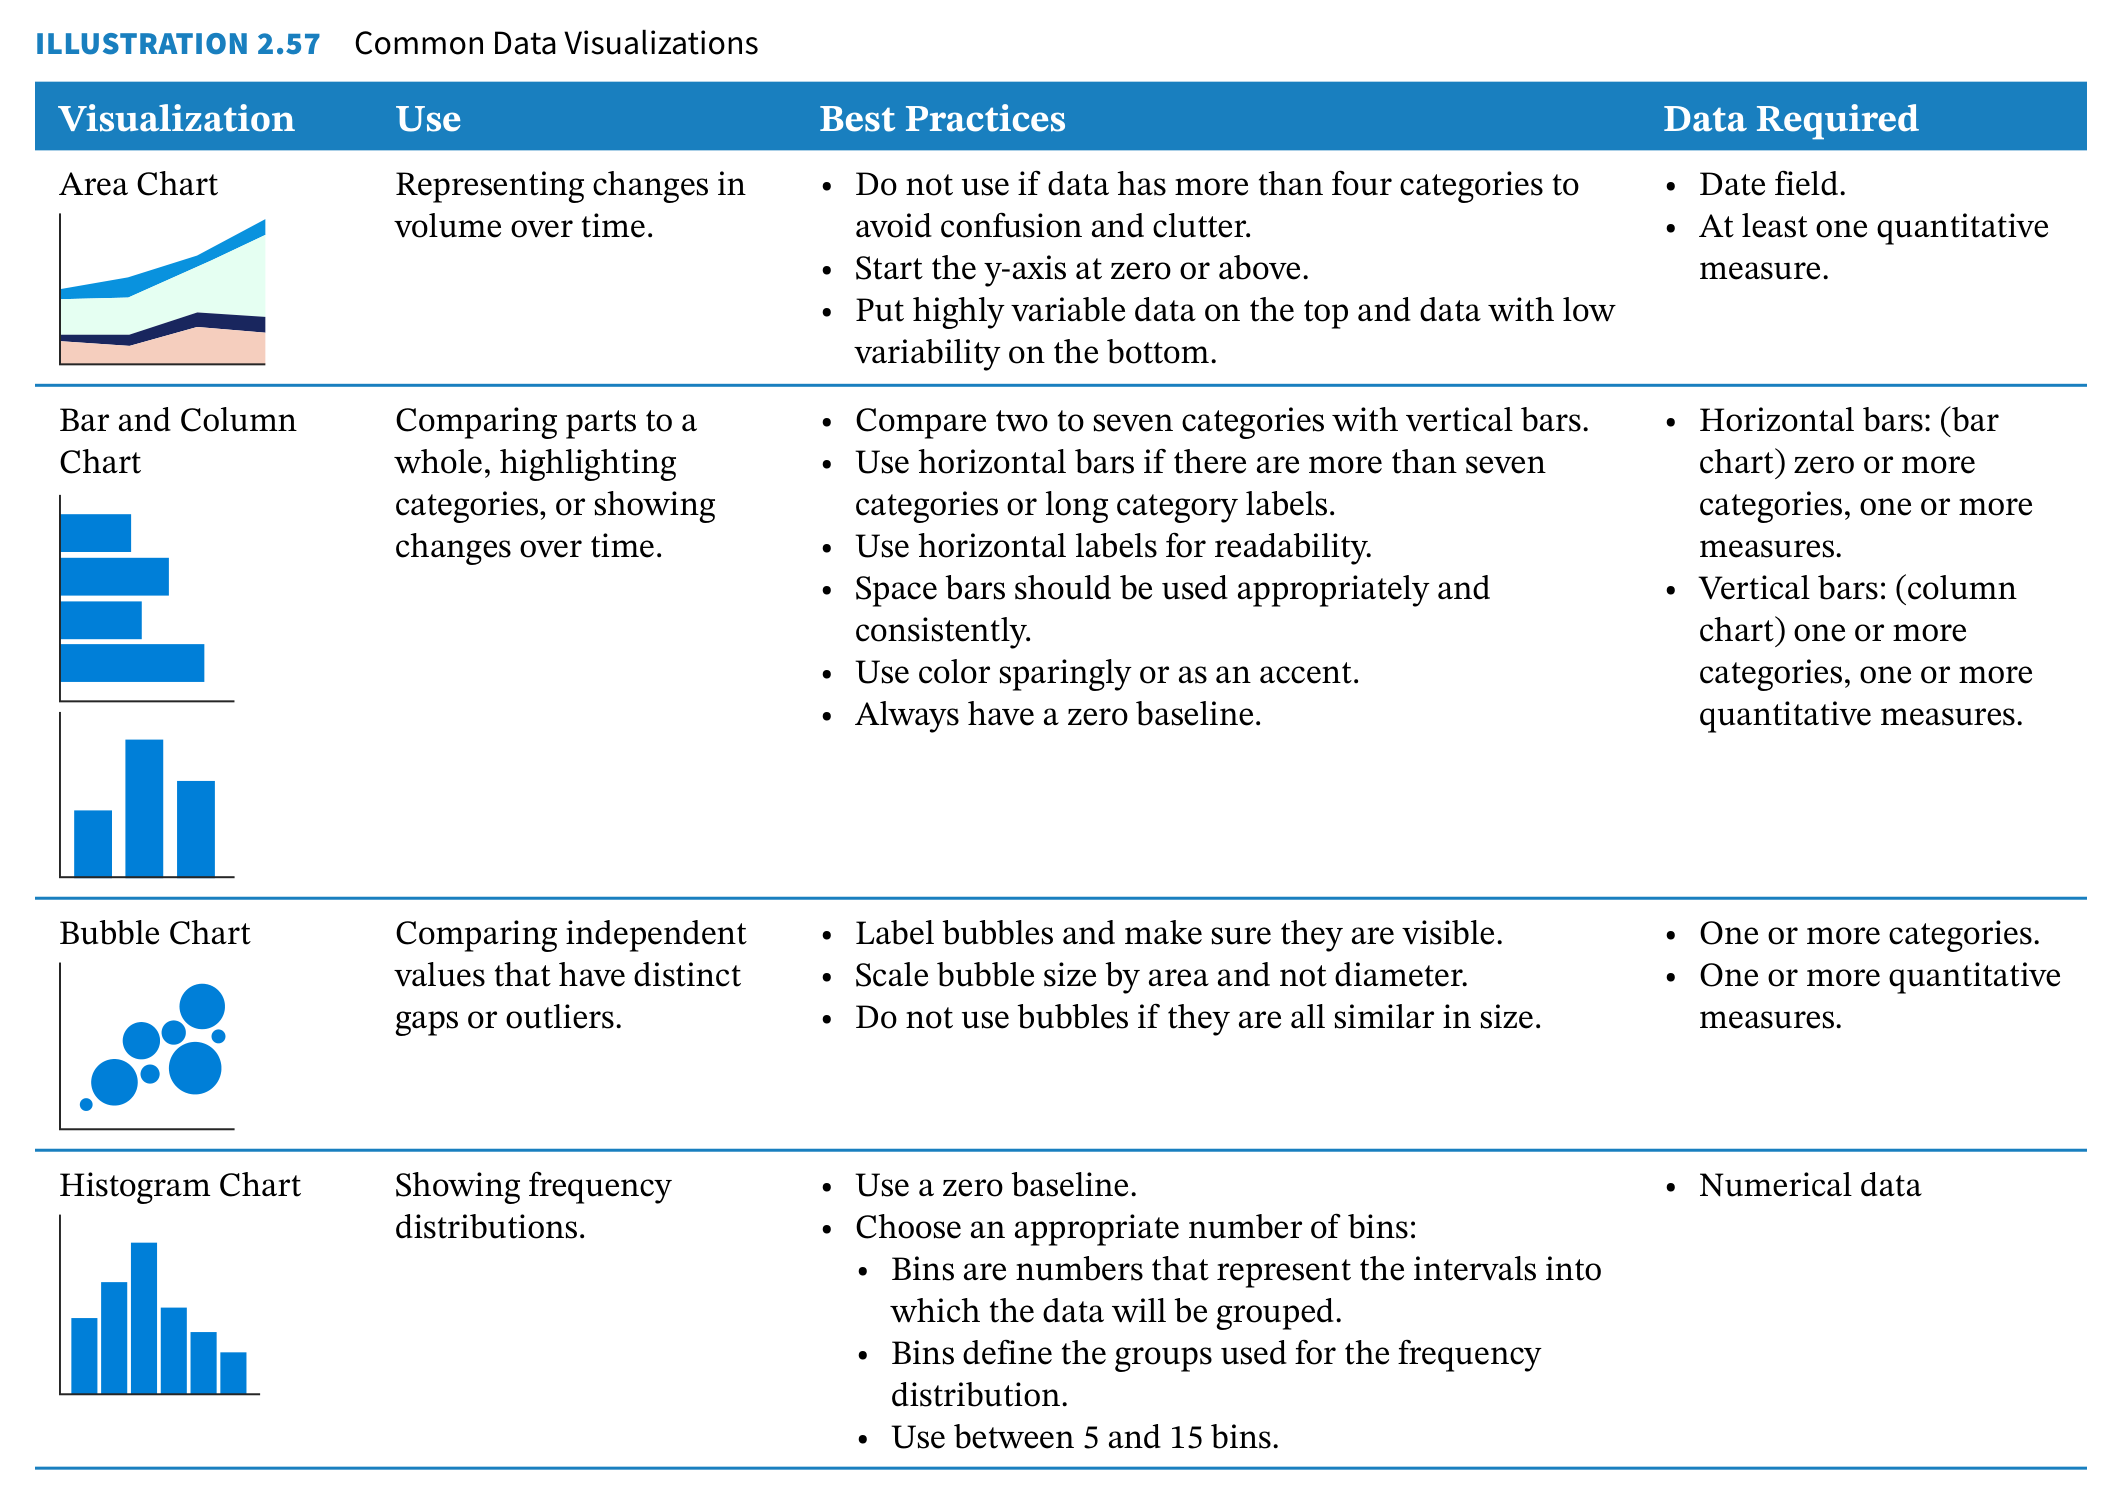
\includegraphics[width=\textwidth]{../textbookForPractice/Figures/Ch_02/ILLUSTRATION 2.57.png}
                \caption{Biểu đồ Tròn (Pie Chart).}
            \end{figure}
        \end{column}
        \begin{column}{0.5\textwidth}
            \begin{figure}[h]
                \centering
                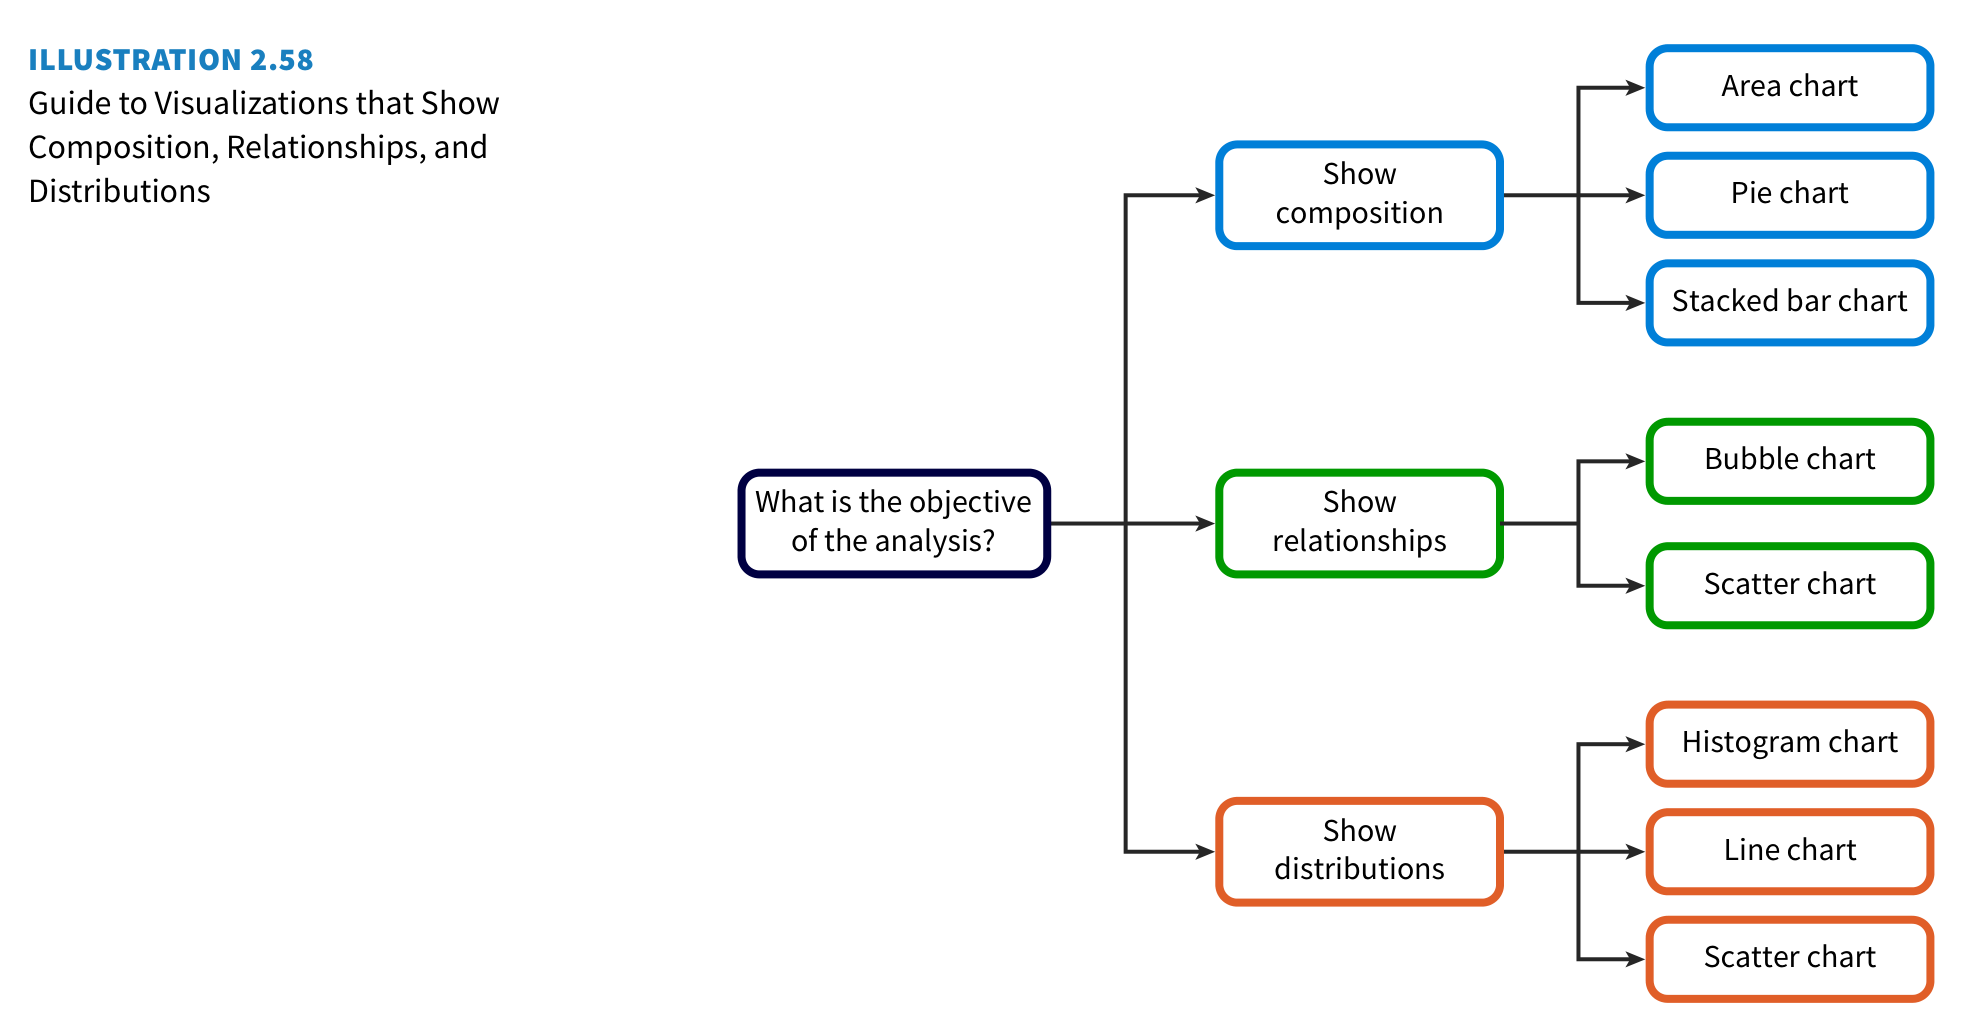
\includegraphics[width=\textwidth]{../textbookForPractice/Figures/Ch_02/ILLUSTRATION 2.58.png}
                \caption{Biểu đồ Đường (Line Chart).}
            \end{figure}
        \end{column}
    \end{columns}
\end{frame}

% --- Phần Bài tập Thực hành ---
\begin{frame}{Đánh giá và Thực hành Chương 2}
    \begin{center}
        \Large \textbf{Phần Bài tập Thực hành (Practice \& Exercises)}
    \end{center}
\end{frame}

\begin{frame}{Bài tập Ngắn (Brief Exercises)}
    \begin{columns}
        \begin{column}{0.5\textwidth}
            \begin{figure}[h]
                \centering
                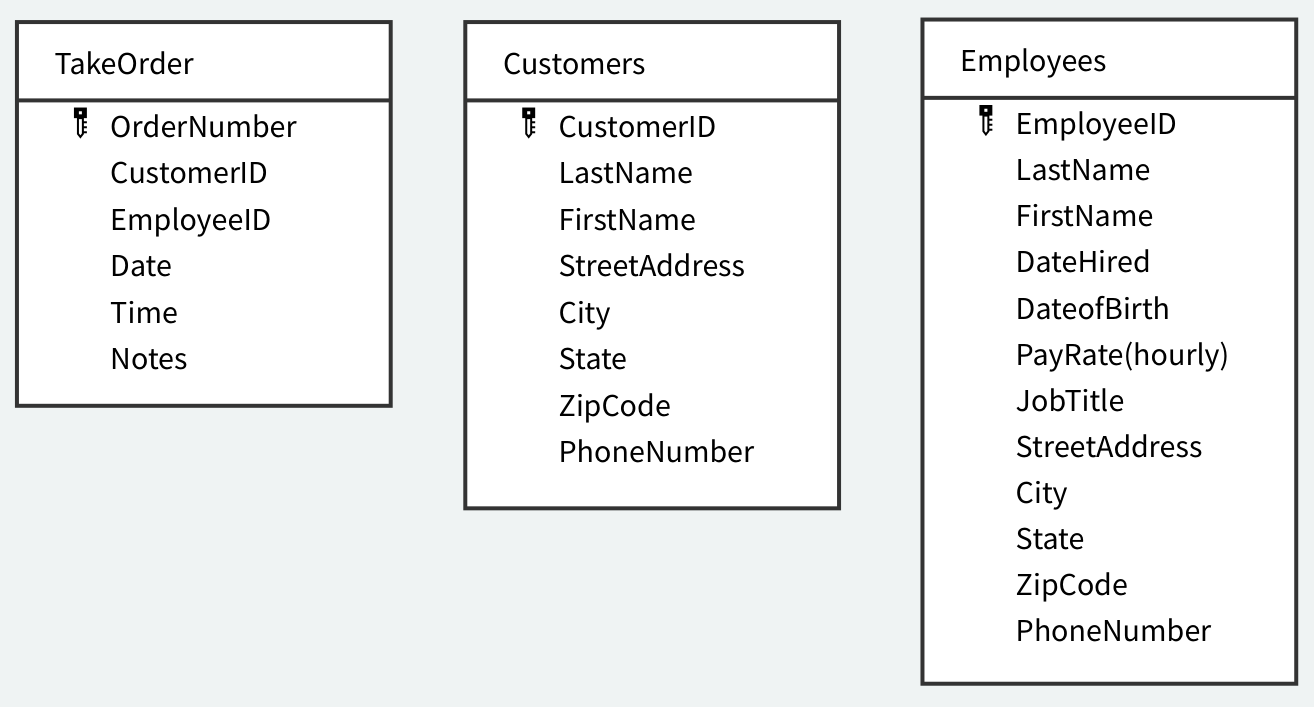
\includegraphics[width=\textwidth]{../textbookForPractice/Figures/Ch_02/BE 2.1.png}
                \caption{BE 2.1}
            \end{figure}
        \end{column}
        \begin{column}{0.5\textwidth}
            \begin{figure}[h]
                \centering
                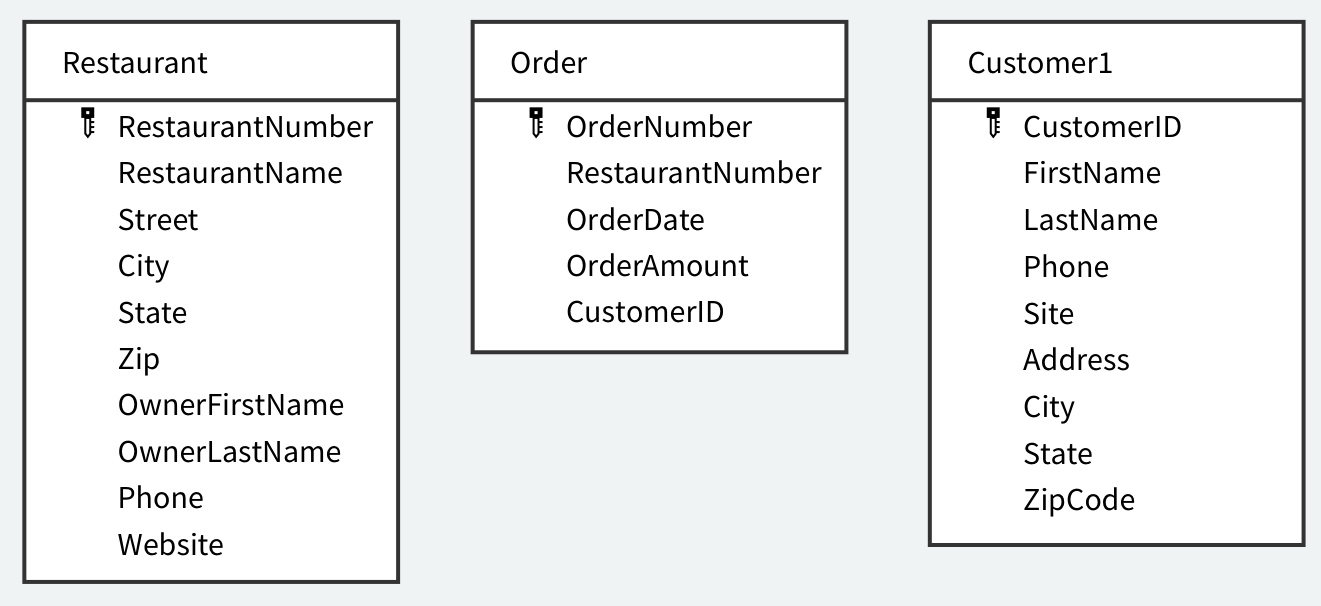
\includegraphics[width=\textwidth]{../textbookForPractice/Figures/Ch_02/BE 2.2.png}
                \caption{BE 2.2}
            \end{figure}
        \end{column}
    \end{columns}
\end{frame}

\begin{frame}{Bài tập (Exercises - EX 2.1 \& EX 2.2)}
    \begin{columns}
        \begin{column}{0.5\textwidth}
            \begin{figure}[h]
                \centering
                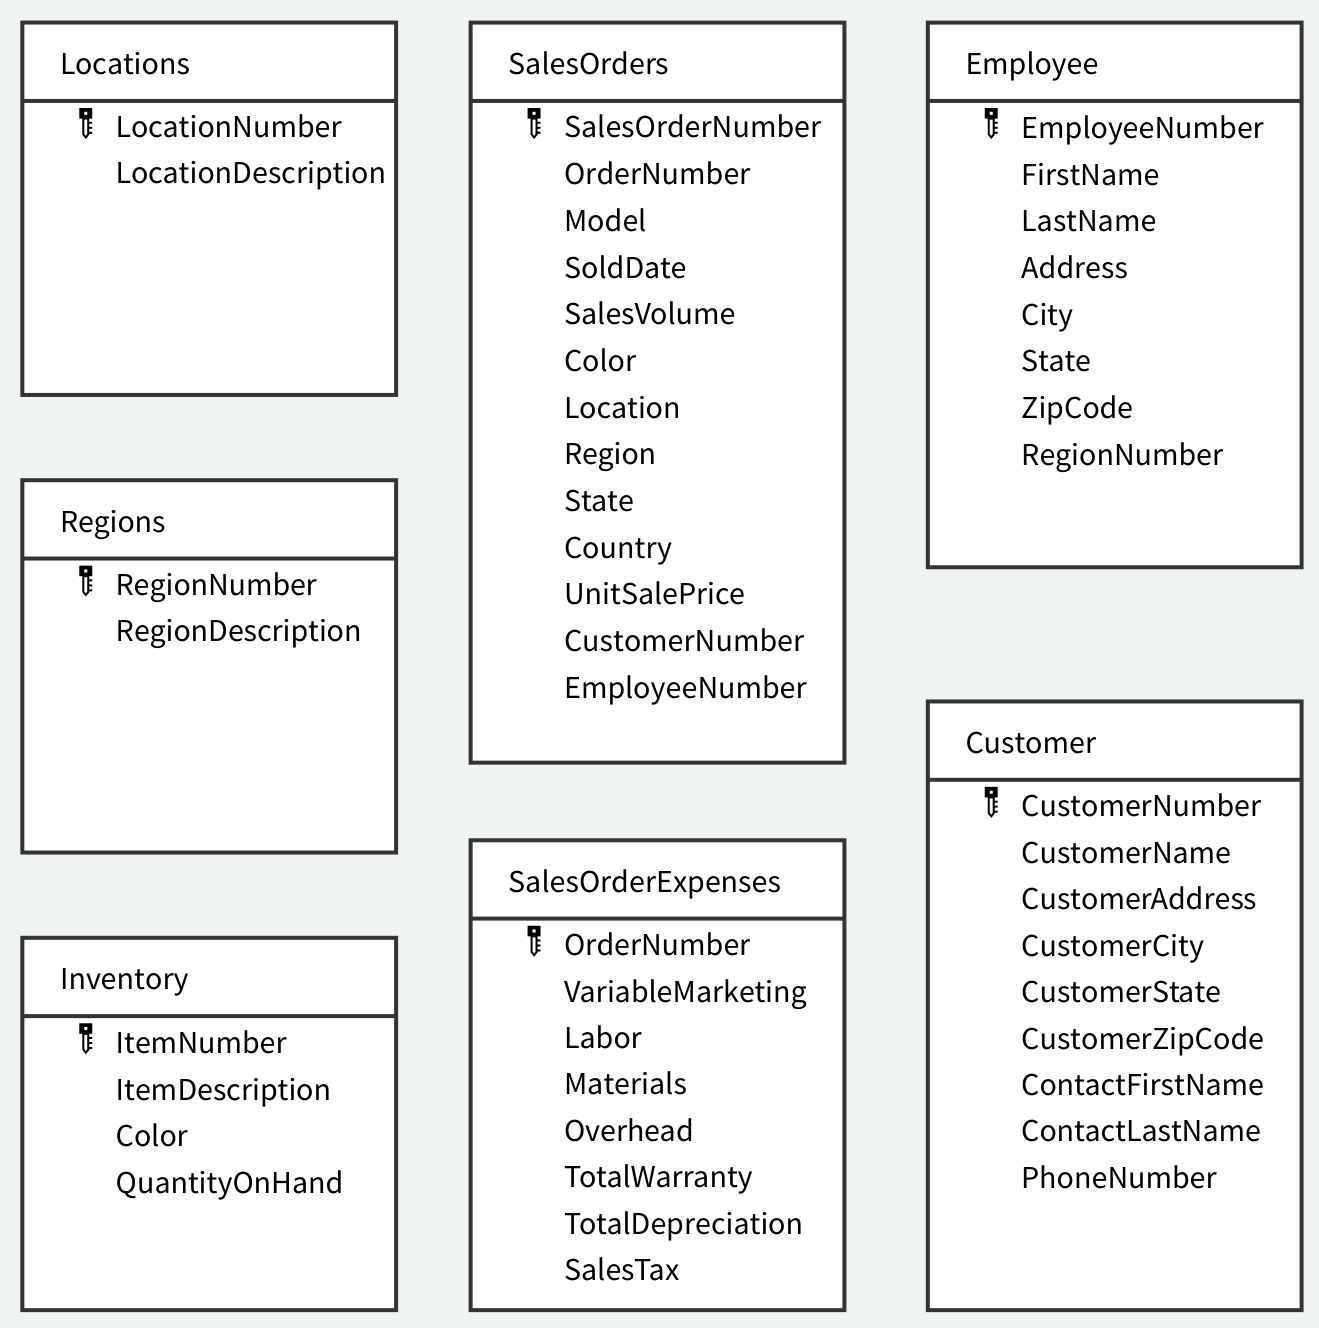
\includegraphics[width=\textwidth]{../textbookForPractice/Figures/Ch_02/EX 2.1.png}
                \caption{EX 2.1}
            \end{figure}
        \end{column}
        \begin{column}{0.5\textwidth}
            \begin{figure}[h]
                \centering
                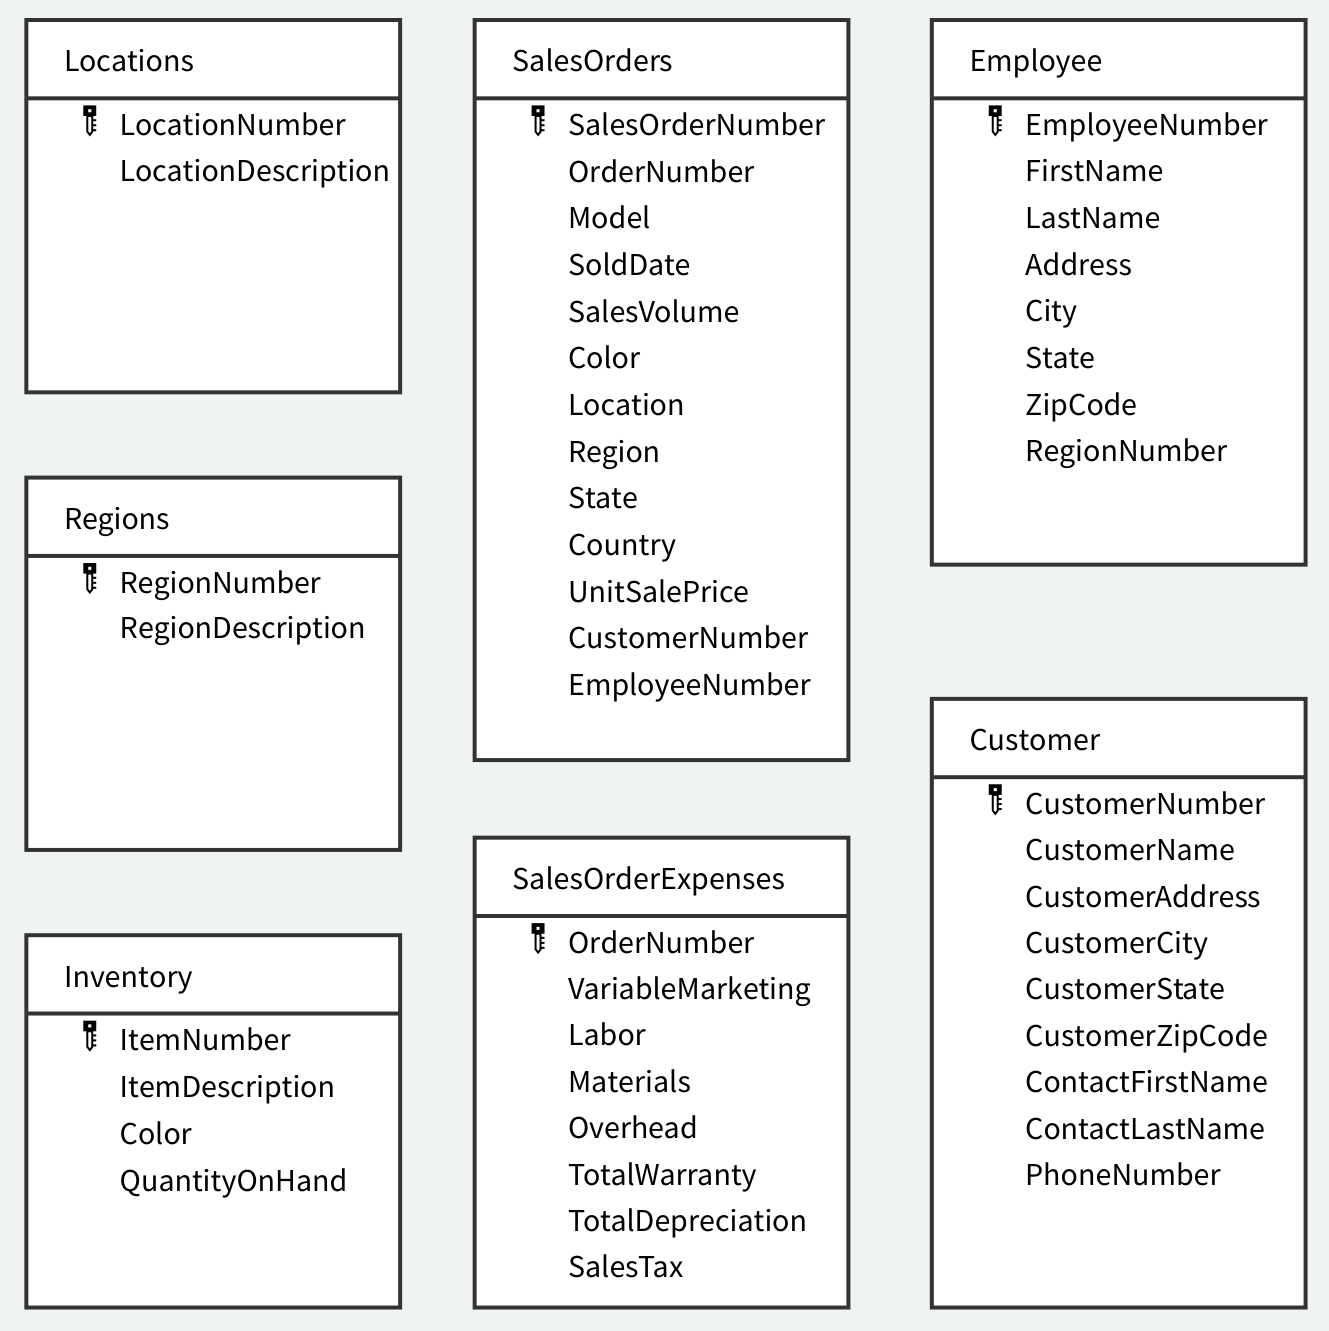
\includegraphics[width=\textwidth]{../textbookForPractice/Figures/Ch_02/EX 2.2.png}
                \caption{EX 2.2}
            \end{figure}
        \end{column}
    \end{columns}
\end{frame}

\begin{frame}{Bài tập (Exercises - EX 2.3 \& EX 2.4)}
    \begin{columns}
        \begin{column}{0.5\textwidth}
            \begin{figure}[h]
                \centering
                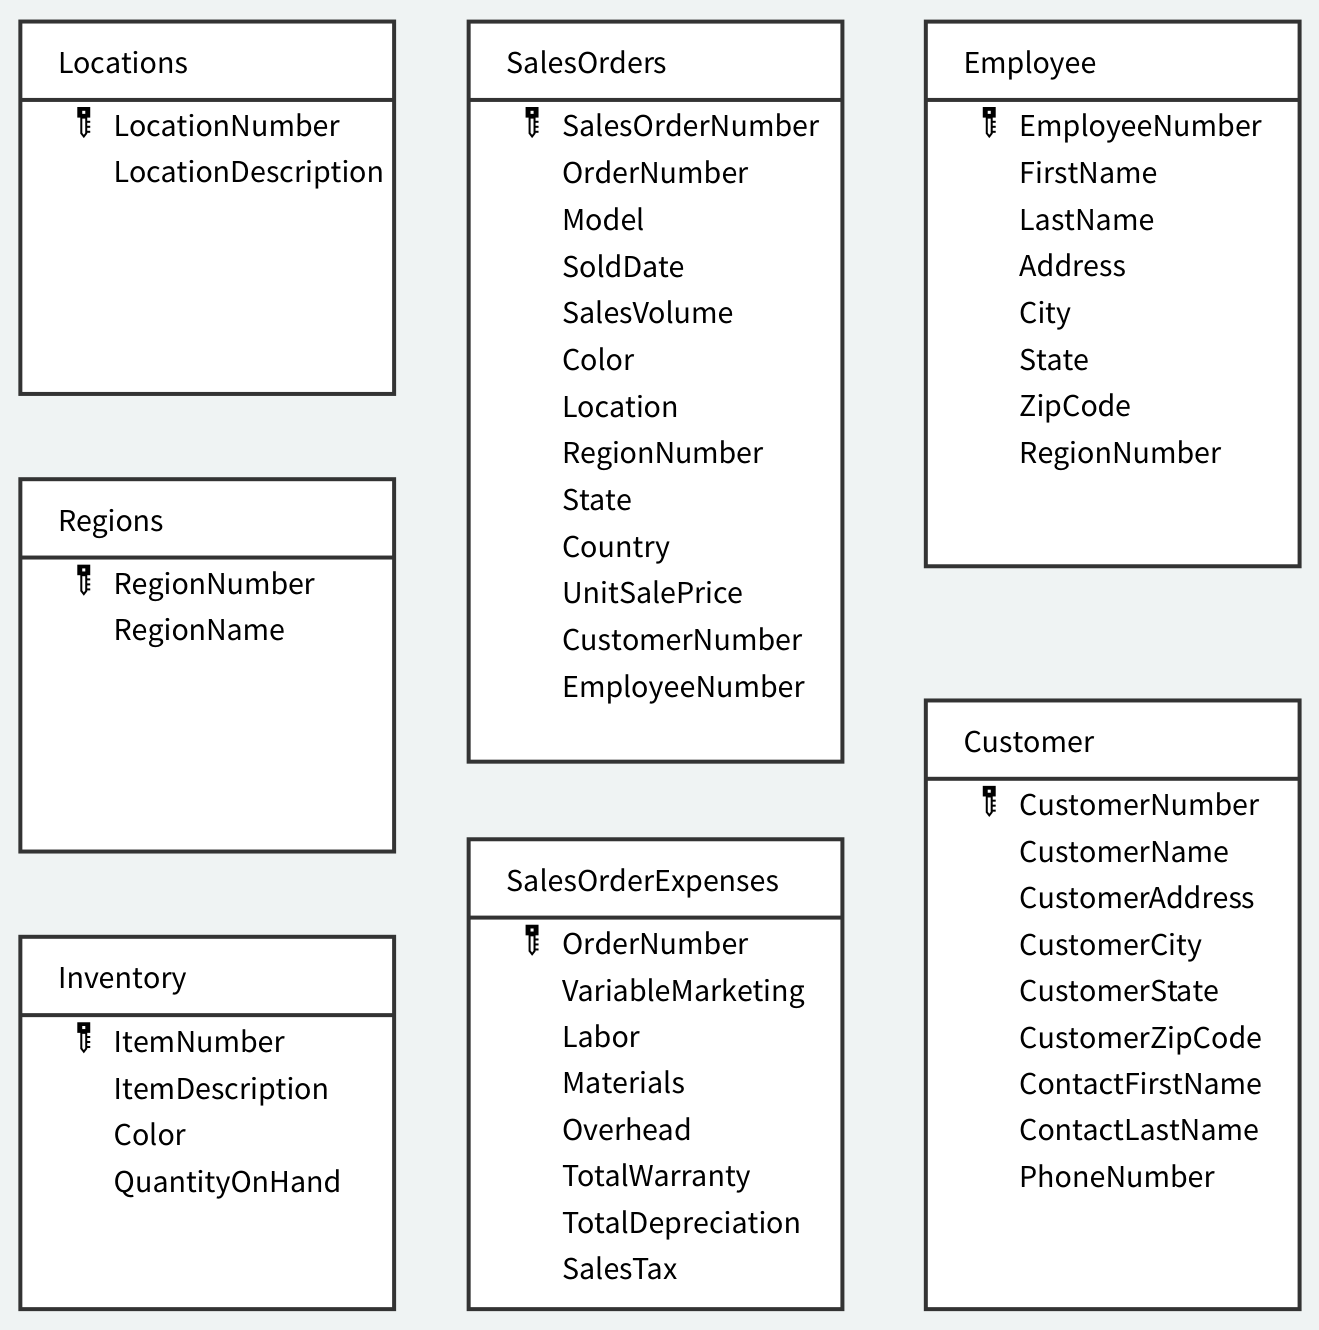
\includegraphics[width=\textwidth]{../textbookForPractice/Figures/Ch_02/EX 2.3.png}
                \caption{EX 2.3}
            \end{figure}
        \end{column}
        \begin{column}{0.5\textwidth}
            \begin{figure}[h]
                \centering
                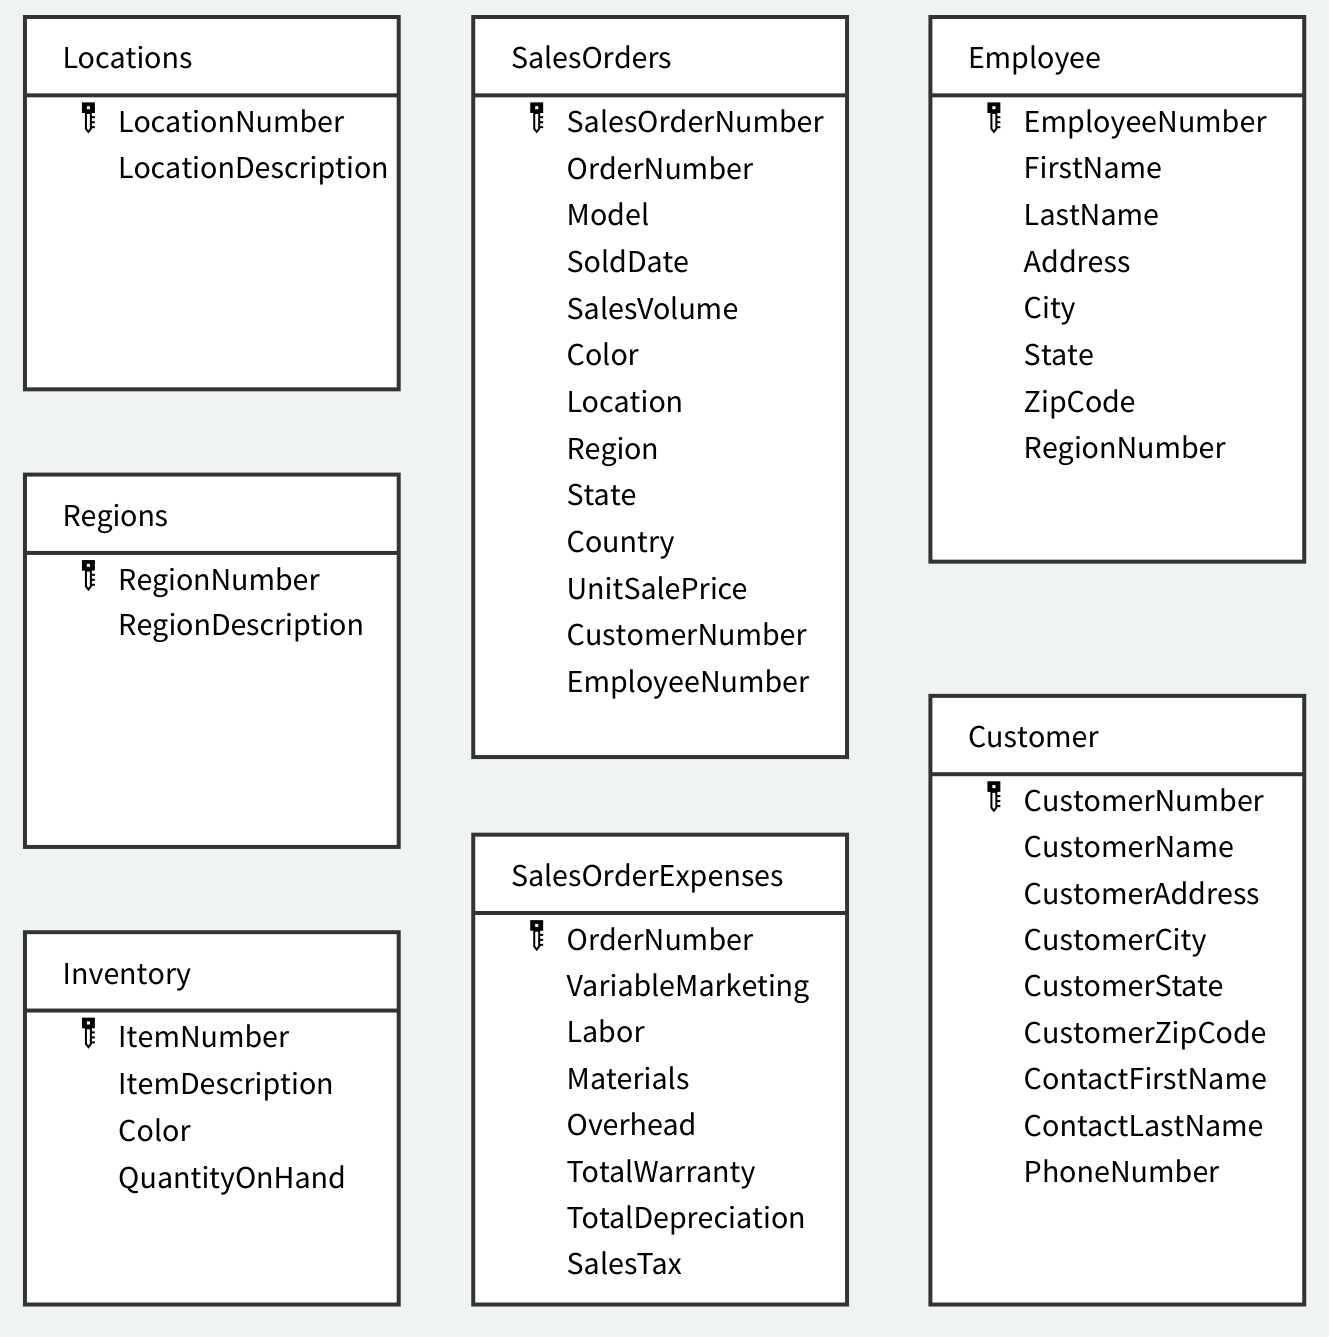
\includegraphics[width=\textwidth]{../textbookForPractice/Figures/Ch_02/EX 2.4.png}
                \caption{EX 2.4}
            \end{figure}
        \end{column}
    \end{columns}
\end{frame}

% --- Tình huống Ứng dụng Chuyên môn ---
\begin{frame}{Tình huống Ứng dụng Chuyên môn (PAC)}
    \begin{center}
        \Large \textbf{Pizza My Heart Food Truck}
    \end{center}
\end{frame}

\begin{frame}{Dữ liệu Tình huống}
    \begin{figure}[h]
        \centering
        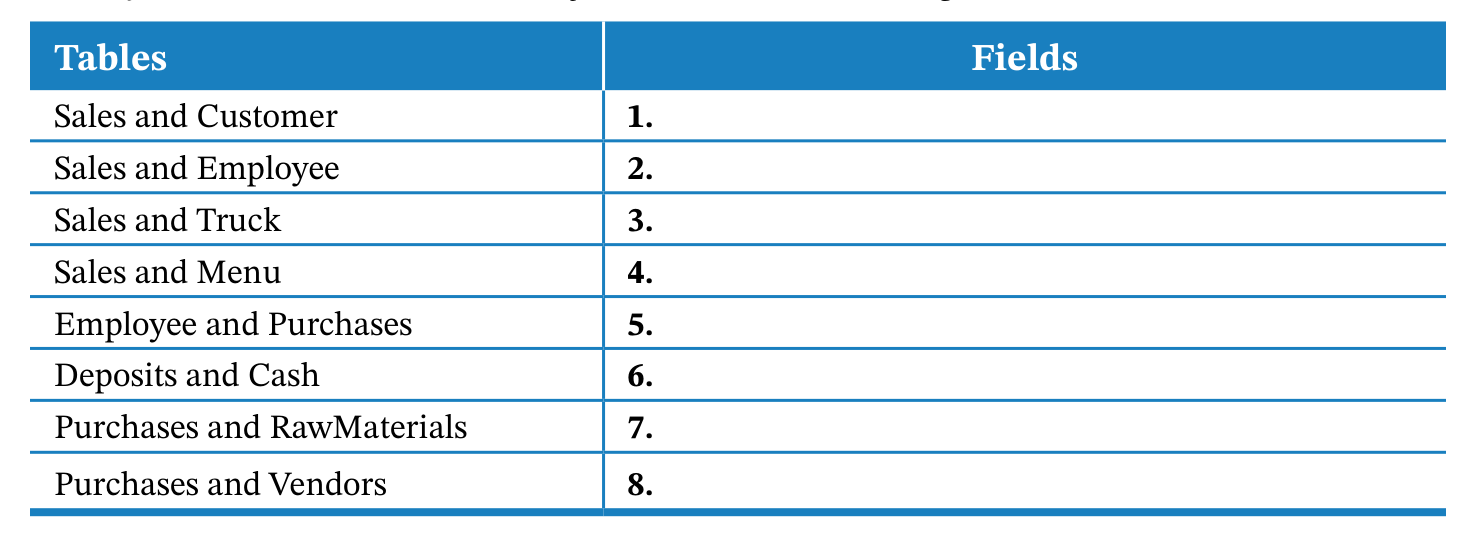
\includegraphics[height=0.7\textheight,keepaspectratio]{../textbookForPractice/Figures/Ch_02/PAC 2.1A.png}
        \caption{Yêu cầu PAC 2.1 - Pizza My Heart Database.}
    \end{figure}
\end{frame}

\begin{frame}{Dữ liệu Tình huống (Tiếp)}
    \begin{figure}[h]
        \centering
        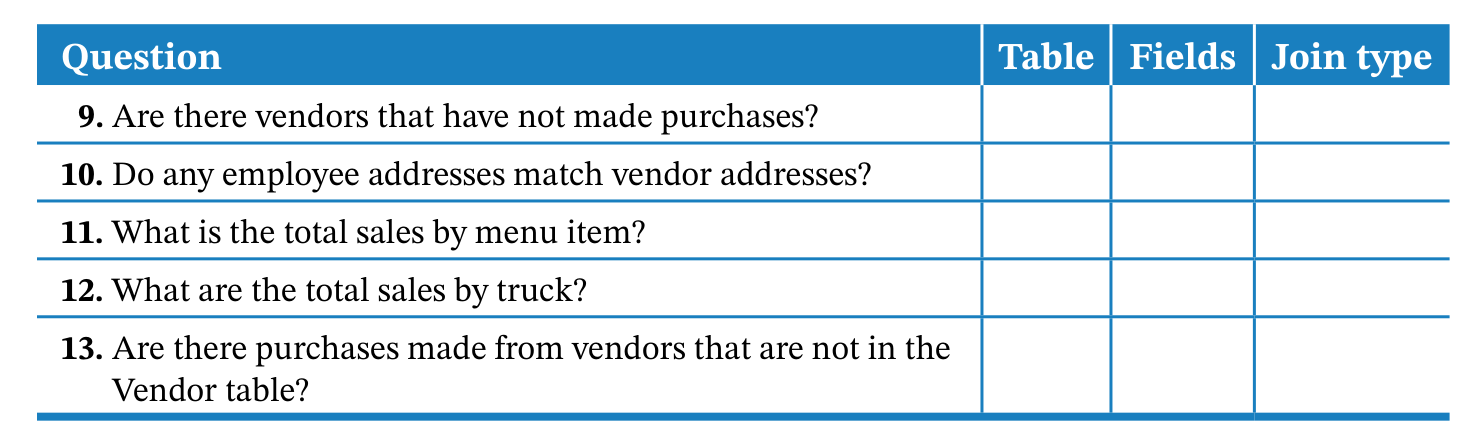
\includegraphics[height=0.7\textheight,keepaspectratio]{../textbookForPractice/Figures/Ch_02/PAC 2.1B.png}
        \caption{Tiếp tục PAC 2.1 - Table Properties.}
    \end{figure}
\end{frame}

\begin{frame}{Kết thúc}
    \begin{center}
        \Huge \textbf{Hỏi \& Đáp} \\
        \vspace{1cm}
        \Large Cảm ơn các bạn đã lắng nghe!
    \end{center}
\end{frame}

\end{document}
